\documentclass[12pt]{report}
%DIF LATEXDIFF DIFFERENCE FILE
%DIF DEL old.tex   Sat Jun 28 16:26:29 2025
%DIF ADD new.tex   Sat Jun 28 17:04:57 2025

\usepackage{xcolor}
\usepackage{setspace}
\usepackage{pifont}
\usepackage{graphicx} 
\usepackage{tabularx}
\usepackage{float}
\usepackage{enumitem}
\usepackage{hyperref}
\usepackage{listings}
\usepackage{minted}
\usepackage{amsmath}  \usepackage{amssymb}  \usepackage{listings} \usepackage{xcolor}   \usepackage{adjustbox}
\usepackage{multirow}
\usepackage{hyperref}
%DIF 16a16
\usepackage[T1]{fontenc} %DIF > 
%DIF -------
\newcommand{\cmark}{\ding{51}} \newcommand{\xmark}{\ding{55}} \newcommand{\etal}{et~al.\ }

\usepackage[acronym]{glossaries}
\usepackage[left=1.5in, right=1in, top=1in, bottom=1in]{geometry}
\newacronym[plural={VMs}, firstplural={virtual machines (VMs)}]{vm}{VM}{virtual machine}
\makeglossaries
%DIF PREAMBLE EXTENSION ADDED BY LATEXDIFF
%DIF UNDERLINE PREAMBLE %DIF PREAMBLE
\RequirePackage[normalem]{ulem} %DIF PREAMBLE
\RequirePackage{color}\definecolor{RED}{rgb}{1,0,0}\definecolor{BLUE}{rgb}{0,0,1} %DIF PREAMBLE
\providecommand{\DIFaddtex}[1]{{\protect\color{blue}\uwave{#1}}} %DIF PREAMBLE
\providecommand{\DIFdeltex}[1]{{\protect\color{red}\sout{#1}}}                      %DIF PREAMBLE
%DIF SAFE PREAMBLE %DIF PREAMBLE
\providecommand{\DIFaddbegin}{} %DIF PREAMBLE
\providecommand{\DIFaddend}{} %DIF PREAMBLE
\providecommand{\DIFdelbegin}{} %DIF PREAMBLE
\providecommand{\DIFdelend}{} %DIF PREAMBLE
\providecommand{\DIFmodbegin}{} %DIF PREAMBLE
\providecommand{\DIFmodend}{} %DIF PREAMBLE
%DIF FLOATSAFE PREAMBLE %DIF PREAMBLE
\providecommand{\DIFaddFL}[1]{\DIFadd{#1}} %DIF PREAMBLE
\providecommand{\DIFdelFL}[1]{\DIFdel{#1}} %DIF PREAMBLE
\providecommand{\DIFaddbeginFL}{} %DIF PREAMBLE
\providecommand{\DIFaddendFL}{} %DIF PREAMBLE
\providecommand{\DIFdelbeginFL}{} %DIF PREAMBLE
\providecommand{\DIFdelendFL}{} %DIF PREAMBLE
%DIF HYPERREF PREAMBLE %DIF PREAMBLE
\providecommand{\DIFadd}[1]{\texorpdfstring{\DIFaddtex{#1}}{#1}} %DIF PREAMBLE
\providecommand{\DIFdel}[1]{\texorpdfstring{\DIFdeltex{#1}}{}} %DIF PREAMBLE
\newcommand{\DIFscaledelfig}{0.5}
%DIF HIGHLIGHTGRAPHICS PREAMBLE %DIF PREAMBLE
\RequirePackage{settobox} %DIF PREAMBLE
\RequirePackage{letltxmacro} %DIF PREAMBLE
\newsavebox{\DIFdelgraphicsbox} %DIF PREAMBLE
\newlength{\DIFdelgraphicswidth} %DIF PREAMBLE
\newlength{\DIFdelgraphicsheight} %DIF PREAMBLE
% store original definition of \includegraphics %DIF PREAMBLE
\LetLtxMacro{\DIFOincludegraphics}{\includegraphics} %DIF PREAMBLE
\newcommand{\DIFaddincludegraphics}[2][]{{\color{blue}\fbox{\DIFOincludegraphics[#1]{#2}}}} %DIF PREAMBLE
\newcommand{\DIFdelincludegraphics}[2][]{% %DIF PREAMBLE
\sbox{\DIFdelgraphicsbox}{\DIFOincludegraphics[#1]{#2}}% %DIF PREAMBLE
\settoboxwidth{\DIFdelgraphicswidth}{\DIFdelgraphicsbox} %DIF PREAMBLE
\settoboxtotalheight{\DIFdelgraphicsheight}{\DIFdelgraphicsbox} %DIF PREAMBLE
\scalebox{\DIFscaledelfig}{% %DIF PREAMBLE
\parbox[b]{\DIFdelgraphicswidth}{\usebox{\DIFdelgraphicsbox}\\[-\baselineskip] \rule{\DIFdelgraphicswidth}{0em}}\llap{\resizebox{\DIFdelgraphicswidth}{\DIFdelgraphicsheight}{% %DIF PREAMBLE
\setlength{\unitlength}{\DIFdelgraphicswidth}% %DIF PREAMBLE
\begin{picture}(1,1)% %DIF PREAMBLE
\thicklines\linethickness{2pt} %DIF PREAMBLE
{\color[rgb]{1,0,0}\put(0,0){\framebox(1,1){}}}% %DIF PREAMBLE
{\color[rgb]{1,0,0}\put(0,0){\line( 1,1){1}}}% %DIF PREAMBLE
{\color[rgb]{1,0,0}\put(0,1){\line(1,-1){1}}}% %DIF PREAMBLE
\end{picture}% %DIF PREAMBLE
}\hspace*{3pt}}} %DIF PREAMBLE
} %DIF PREAMBLE
\LetLtxMacro{\DIFOaddbegin}{\DIFaddbegin} %DIF PREAMBLE
\LetLtxMacro{\DIFOaddend}{\DIFaddend} %DIF PREAMBLE
\LetLtxMacro{\DIFOdelbegin}{\DIFdelbegin} %DIF PREAMBLE
\LetLtxMacro{\DIFOdelend}{\DIFdelend} %DIF PREAMBLE
\DeclareRobustCommand{\DIFaddbegin}{\DIFOaddbegin \let\includegraphics\DIFaddincludegraphics} %DIF PREAMBLE
\DeclareRobustCommand{\DIFaddend}{\DIFOaddend \let\includegraphics\DIFOincludegraphics} %DIF PREAMBLE
\DeclareRobustCommand{\DIFdelbegin}{\DIFOdelbegin \let\includegraphics\DIFdelincludegraphics} %DIF PREAMBLE
\DeclareRobustCommand{\DIFdelend}{\DIFOaddend \let\includegraphics\DIFOincludegraphics} %DIF PREAMBLE
\LetLtxMacro{\DIFOaddbeginFL}{\DIFaddbeginFL} %DIF PREAMBLE
\LetLtxMacro{\DIFOaddendFL}{\DIFaddendFL} %DIF PREAMBLE
\LetLtxMacro{\DIFOdelbeginFL}{\DIFdelbeginFL} %DIF PREAMBLE
\LetLtxMacro{\DIFOdelendFL}{\DIFdelendFL} %DIF PREAMBLE
\DeclareRobustCommand{\DIFaddbeginFL}{\DIFOaddbeginFL \let\includegraphics\DIFaddincludegraphics} %DIF PREAMBLE
\DeclareRobustCommand{\DIFaddendFL}{\DIFOaddendFL \let\includegraphics\DIFOincludegraphics} %DIF PREAMBLE
\DeclareRobustCommand{\DIFdelbeginFL}{\DIFOdelbeginFL \let\includegraphics\DIFdelincludegraphics} %DIF PREAMBLE
\DeclareRobustCommand{\DIFdelendFL}{\DIFOaddendFL \let\includegraphics\DIFOincludegraphics} %DIF PREAMBLE
%DIF COLORLISTINGS PREAMBLE %DIF PREAMBLE
\RequirePackage{listings} %DIF PREAMBLE
\RequirePackage{color} %DIF PREAMBLE
\lstdefinelanguage{DIFcode}{ %DIF PREAMBLE
%DIF DIFCODE_UNDERLINE %DIF PREAMBLE
  moredelim=[il][\color{red}\sout]{\%DIF\ <\ }, %DIF PREAMBLE
  moredelim=[il][\color{blue}\uwave]{\%DIF\ >\ } %DIF PREAMBLE
} %DIF PREAMBLE
\lstdefinestyle{DIFverbatimstyle}{ %DIF PREAMBLE
	language=DIFcode, %DIF PREAMBLE
	basicstyle=\ttfamily, %DIF PREAMBLE
	columns=fullflexible, %DIF PREAMBLE
	keepspaces=true %DIF PREAMBLE
} %DIF PREAMBLE
\lstnewenvironment{DIFverbatim}{\lstset{style=DIFverbatimstyle}}{} %DIF PREAMBLE
\lstnewenvironment{DIFverbatim*}{\lstset{style=DIFverbatimstyle,showspaces=true}}{} %DIF PREAMBLE
%DIF END PREAMBLE EXTENSION ADDED BY LATEXDIFF

\begin{document}
	\title{An Empirical-Based Security Benchmarking Framework for Container Confinement}
\author{Huzaifa Patel}
\date{2025}

\makeatletter
\begin{titlepage}
    \newgeometry{margin=1in} \begin{center}
        \vspace*{3cm} 

        {\LARGE \textbf{\@title} \par} 

        \vspace{0.5cm}

        \vspace{2cm}
        \large{by}
        \vspace{0.5cm}

        {\Large \textbf{\@author}} 

        \vfill

        {\large A thesis submitted to the Faculty of Graduate and Postdoctoral Affairs\\
        in partial fulfillment of the requirements for the degree of}

        \vspace{1cm}

        \large{{\textbf{Master}} \\
        {in} \\
        {\textbf{Computer Science}}}


        \vspace{2cm}

        \large{Carleton University\\
        Ottawa, Ontario}

        \vspace{1.5cm}


        \vfill

        \copyright{}~2025 \@author
    \end{center}
\end{titlepage}
\makeatother 	\tableofcontents
	\DIFaddbegin \listoftables
	\listoffigures
	\DIFaddend \printglossary[type=acronym, title=Nomenclature]
	\fontsize{12pt}{14pt} \selectfont
\begin{doublespace}
\chapter{Introduction}

Container-based workloads have become a cornerstone of modern cloud infrastructure, revolutionizing how applications are developed, deployed, and scaled, particularly within microservices architectures and DevOps workflows. Unlike hypervisor-based virtual machines (VMs), which each require a full operating system and rely on a hypervisor for hardware virtualization, containers are lightweight, share the host system’s kernel, and incur minimal overhead. This efficiency makes them exceptionally well-suited for continuous integration and rapid scaling, allowing organizations to optimize resource utilization and reduce costs while ensuring quick, consistent deployments. Furthermore, containers enable seamless portability by packaging all userspace dependencies into a unified image, thereby avoiding the common problem of environment-specific discrepancies. Yet, despite containers’ numerous benefits, they also introduce new security challenges, especially where container confinement is concerned.

Linux kernel features such as cgroups and namespaces provide resource, process, and network isolation for containers. However, this separation is not foolproof. Kernel vulnerabilities, such as, but not limited to buffer overflows or privilege escalation flaws can allow a process to circumvent the very mechanisms designed to confine it. Misconfigurations can similarly open holes in container security, for instance by granting unnecessary capabilities, mounting sensitive host directories, or running containers in privileged mode. Container escapes exploit these weaknesses to break out of the container’s resource and namespace isolation. Once an attacker gains elevated privileges or direct access to the host system, they can disrupt other containers, exfiltrate data, or compromise the entire infrastructure. 

Technologies like SELinux, AppArmor, and seccomp provide additional layers of host-based security to mitigate these issues but are notoriously prone to misconfiguration. Best practices guides for container security~\cite{CIS} can help but they offer no guarantee that a given configuration will perform as intended by the end user. As container adoption has skyrocketed across industries, particularly in multi-tenant cloud environments, these security challenges have become more pronounced.

To improve container security, the cloud industry has developed technologies like Kata Containers\footnote{\url{https://katacontainers.io}}, which isolate containers further by running them within lightweight VMs. While this approach can be effective, it also adds another layer of complexity which is subject to its own set of vulnerabilities and implementation errors. Simply adding additional layers of security does not, it itself, mean that security goals have been achieved.

Test suites play a crucial role in verifying that systems meet specified requirements and function correctly under defined conditions. They are widely used across computing disciplines, from performance benchmarking to security assessment. For instance, the Standard Performance Evaluation Corporation (SPEC) \cite{henning2000spec} is best known for developing industry-standard benchmarks that evaluate CPU performance and power efficiency, while the Transaction Processing Performance Council (TPC) \cite{10.1007/978-3-642-18206-8_1} establishes benchmarking standards for database performance.
Specialized security-focused test suites play a vital role in detecting vulnerabilities in deployed systems. Tools such as network scanners aid in identifying misconfigurations, outdated software versions, and unintended service exposures, helping organizations proactively mitigate security risks. However, a significant gap remains in the context of containers. There are currently no standardized or widely adopted test suites designed specifically to evaluate container confinement, functionality, or isolation effectiveness. This absence leaves organizations to rely on ad hoc methods, which are often inadequate for uncovering subtle misconfigurations or ensuring robust confinement. Given the growing reliance on containerized environments in modern infrastructure, the development of comprehensive test suites tailored for containers is imperative.

In this paper, we describe Houdini, the first test suite for verifying container confinement. Given a Docker container configuration (including the kernel, docker, and runc version), Houdini will instantiate the container in a standalone QEMU-based VM and perform multiple tests (or \textit{tricks}, as we call them) to evaluate the container's security posture. These tests explore vulnerabilities such as improper resource allocation, inadequate isolation, and insecure filesystem setups. Houdini is written in Python and provides an extension language for writing tricks, allowing it to adapt as new container escape vulnerabilities arise.

\section{Contributions}

This paper makes the following contributions:
\begin{itemize}
    \item Defines container confinement and its associated challenges.
    \item Introduces \textit{Houdini}, a modular framework for testing container security.
    \item Demonstrates Houdini’s ability to detect security issues, misconfigurations, and inconsistencies in container confinement.
\end{itemize}

\section{The Container Confinement Problem}

Container confinement can be defined as the set of mechanisms and strategies used to isolate a containerized application from the host system and other containers. Effective confinement is critical for maintaining system security and stability, as it ensures that containers operate within defined boundaries by restricting their access to system resources including processes, networks, filesystems, devices, and kernel interfaces. 

A challenge with container confinement is that the level of confinement of a container is not fixed; it can vary based on the specific requirements of the user. In other words, the degree to which a container is isolated from the host system or other containers is customizable to meet the user’s needs. At one end of the spectrum, one can lock a container down so tightly that it is almost entirely isolated from the host system, which minimizes potential attack surfaces but can also render the container incapable of performing key tasks. On the other hand, giving a container too many privileges increases the impact of any security compromise. The optimal configuration is one that strikes a balance between maximum confinement (i.e., least privilege) and sufficient functionality. 


A standardized, formal approach involving rigorously evaluating and analyzing the security of the container and its environment might seem ideal; however, it is impractical because container environments are highly complex, with interactions between kernels, runtimes, orchestration tools, and external dependencies that are difficult to model comprehensively. Moreover, many vulnerabilities stem from subtle details that a formal model might overlook. Instead, we believe an empirical approach offers a practical alternative. Although it will likely never be exhaustive, the goal is not comprehensive coverage but rather establishing a baseline set of tests that demonstrate effective container confinement.



\section{Motivation}

Houdini is designed to provide a systematic and reproducible approach to testing container confinement mechanisms. One of its primary goals is to evaluate whether container security features, such as namespaces, cgroups, seccomp, and Linux capabilities are effectively enforcing isolation. Many container security tools rely on theoretical guarantees or static analysis\cite{clair}, but Houdini focuses on empirical validation by executing controlled security tests that verify the correct enforcement of security mechanisms. By doing so, Houdini ensures that container security mechanisms are correctly configured.

Houdini is not only for testing container isolation but also as a means to optimize container configurations. By systematically simulating various tasks within different containers, Houdini can help determine the minimal set of privileges required for a container to perform its intended function. For example, administrators can start with a container configured with broad privileges and then incrementally reduce permissions, such as Linux capabilities, seccomp filters, or resource limits, while monitoring task success. Houdini’s testing framework will identify the point at which functionality is maintained while unnecessary privileges are removed, thereby pinpointing the least privilege configuration that still allows the container to operate effectively. Minimizing the privileges granted to a container reduces its attack surface, making it more difficult for an attacker to exploit vulnerabilities.

Although runtime monitoring and anomaly detection, such as with eBPF-based tracing\cite{findlay2021bpfcontain} can provide immediate insights into container behavior, our goal isn't to implement an exhaustive, continuous surveillance system. Instead, we aim to focus on auditing and validating the underlying isolation mechanisms to ensure they are correctly configured and consistently enforced.

\subsection{Example Applications of Houdini}
A system like Houdini can be used in the following ways: 

\noindent\textbf{Identify gaps between intended confinement policies and actual enforcement:}
There is often a discrepancy between the security policies that administrators intend to enforce and what is actually upheld at runtime. These discrepancies generally fall into two categories: implicit policy problems and conflicting policy configurations.

An implicit policy problem happens when an administrator doesn't explicitly set a security rule, and the system's default behavior is used instead. These defaults might lead to behavior the administrator did not expect. For example, Docker containers are, by default, connected to a shared internal bridge network. While this topology typically prevents internet access, it still allows containers to communicate with each other. An administrator might see that outbound traffic from a container is blocked and mistakenly believe the container is fully isolated from other networks. However, internal communication between containers will still be allowed unless it's explicitly disabled. Thus, this default behavior can create a false sense of security and introduce unexpected risks.

A conflicting policy configuration, on the other hand, occurs when a security policy is correctly specified but is later invalidated by other conflicting configurations. For example, an administrator might launch a container with \texttt{--network=none}, expecting it to be fully isolated from all network communication. However, if the container is also inadvertently given elevated privileges such as \texttt{--cap-add=NET\_ADMIN} or \texttt{--privileged}, it can reconfigure its own network interfaces and regain connectivity. With the \texttt{NET\_ADMIN} capability, processes inside the container gain access to low-level networking operations, such as creating virtual interfaces, assigning IP addresses, or modifying routing tables. A process could use commands like \texttt{ip link set eth0 up} and \texttt{dhclient eth0} to bring up a previously disabled interface and request an IP address from the host’s network. In the case of a \texttt{--privileged} container, even more capabilities are granted, allowing near-complete access to the host's kernel features, including the creation of new network namespaces or interfaces, effectively bypassing the isolation intended by \texttt{--network=none}.

Houdini can help identify these gaps by systematically testing the behavior of the container against the intended security policies, as demonstrated in case study 2 in .

\noindent\textbf{Challenge misleading security assumptions with empirical testing:}
Container security is often discussed in terms of theoretical guarantees, with many security best practices based on assumptions rather than direct testing. For instance, documentation may state that a container running in unprivileged mode cannot escalate to root, but Houdini actively tests whether that is actually the case under different container configurations. By running real-world security validation instead of relying solely on security claims, Houdini helps challenge misleading assumptions and exposes where security mechanisms fail in practice. This is particularly important as container escapes and privilege escalation exploits continue to emerge, demonstrating that security controls do not always work as expected. By grounding security claims in measurable results rather than theory, Houdini helps researchers and practitioners develop more robust container security strategies.

\noindent\textbf{Detect security drift over time:} One of the challenges in maintaining secure containerized environments is configuration drift. Security settings applied during container initialization may be inadvertently changed through image updates, runtime automation, or infrastructure changes. Houdini can be set up to periodically re-evaluate security policies, making it possible to detect when the system diverges from its originally intended security posture. This allows for the timely remediation of regressions that could otherwise go unnoticed. Configuration drift does not only arise from explicit policy changes, but also from underlying updates to system components such as the Linux kernel, Docker, or runc. Even when container configurations and security policies remain unchanged, an upgrade to the kernel or container runtime can subtly alter the enforcement of isolation primitives, security defaults, or available capabilities. For example, a new kernel version may modify the behavior of namespaces, cgroups, or seccomp filters; a Docker update may introduce new features or alter default permissions.

\subsection{Design Goals}
In order to support the use cases mentioned above, we designed Houdini with the following goals:

\begin{enumerate}
  \item \label{dg:repro}\textit{Reproducible Results.} A key goal of Houdini is to ensure that tests yield consistent and repeatable results. By controlling system variables and maintaining a structured testing environment, Houdini allows researchers and practitioners to compare results across different system configurations and security policies.

  \item \label{dg:container}\textit{Separation from the Host.} Houdini is designed to run tests inside a controlled containerized environment within a virtual machine (VM), ensuring that even if a trick triggers a security vulnerability, it does not compromise the host system running the tests. This design choice enhances the safety of security evaluations, preventing unintended side effects on the underlying infrastructure.

  \item \label{dg:test}\textit{Test Case Expressiveness.} Houdini tricks should be maximally expressive, such that some combination of steps can be used to achieve and test any desired result. It should be possible to define a new Houdini trick and modify existing tricks without modifying the Houdini binary. Moreover, it should be clear from reading a defined trick precisely what steps are involved, the consequences of each step passing or failing, and the overall nature of the exploit being tested.

  \item \label{dg:failures}\textit{Focus on Observing Failures, Not Preventing Them.} Houdini is built to identify security weaknesses rather than defend against attacks.
\end{enumerate}

\end{doublespace} 	\fontsize{12pt}{14pt} \selectfont
\begin{doublespace}
\chapter{Background \& Related Work}





The existance of cloud computing can be attributed to virtualization, which is a technology that makes it possible for multiple different operating systems (OSs) to run concurrently, and in an isolated environment on the same hardware. How does virtualization achieve this? It makes use of a machines hardware to support the software that creates and manages virtual machines (VMs). A \gls{vm} is a virtual environment that provides the functionality of a physical computer by using its own virtual central processing unit (VCPU), memory, network interface, and storage. The software that creates and manages \glspl{vm} is formally called a hypervisor or virtual machine monitor (VMM). The virtualization marketplace is comprised of four notable hypervisors, which are: (1) VMWare, (2) Xen, (3) Kernel-based Virtual Machine (KVM), and (4) Hyper-V. The operating system running a hypervisor is called the host OS, while the VM that uses the hypervisor is called the guest OS. To maintain consistency within this proposal, we will use the word "hypervisor" when referring to virtualization software. Hypervisors can be divided into two types, depending on where they are located on the machine: (1) type 1 and (2) type 2.

\section{Type 1 Hypervisor}

Type 1 hypervisors run directly on physical hardware to create, control, and manage VMs, and do not require support from the host OS. Type 1 hypervisors are also called native or bare-metal hypervisors. The first hypervisors, which IBM developed in the 1960s were type 1 hypervisors ~\cite{meier2008ibm}. Examples of type 1 hypervisors include, but are not limited to Xen, KVM, VMware ESX, and Microsoft Hyper-V ~\cite{bauman2015survey}.


\section{Type 2 Hypervisor}

Type 2 hypervisors (also called hosted hypervisors) are installed on the OS (Windows, Linux, MacOS), similar to how computer programs are installed onto an OS. In other words, a type 2 hypervisor runs as a process on the host OS. Type 2 hypervisors abstract guest OSs from the host OS by introducing a third software layer above the hardware, as shown in figure 2.1. Examples of type 2 hypervisors include but are not limited to VMware Workstation, VirtualBox, and QEMU ~\cite{bauman2015survey}.





\section{Problems With Type 1 \& Type 2 Hypervisor Classifications}

Although the definitions of type 1 and type 2 hypervisors are widely accepted, there are gray areas where the distinction between the two remain unclear. For instance, according to its creator RedHat, KVM is implemented and deployed using two Linux kernel modules that effectively convert the host Linux OS into a type-1 hypervisor ~\cite{graziano2011performance}. At the same time, KVM can be categorized as a type 2 hypervisor because KVM VM's are standard Linux processes that are competing with other Linux processes for CPU time given by the Linux kernel's native CPU scheduler ~\cite{kvmcpuschedule}. Due to disagreements and vagueness in the definitions of type 1 and type 2 hypervisors, two new classifications were defined: (1) native hypervisors and (2) emulation hypervisors ~\cite{10.1145/2775111}.



\section{Native Hypervisor}

Native hypervisors are hypervisors that push VM guest instructions directly to the physical machines CPU, by using virtualization extensions like Intel VT-x. ~\cite{10.1145/2775111}. Examples of Native hypervisors include but are not limited to Xen, KVM, VMware ESX, and Microsoft HyperV.


\section{Emulation Hypervisor}
Emulation hypervisors are hypervisors that emulate every VM guest instruction using software virtualization ~\cite{10.1145/2775111}. Emulated guest instructions are very easy to trace because all guest VM instructions are trapped to the hypervisor. Examples of emulation hypervisors include but are not limited to QEMU, Bochs, early versions of VMware-Workstation, and VirtualBox ~\cite{10.1145/2775111}.


\section{Why do we have run Docker with sudo?}

By default, Docker’s daemon (dockerd) runs as root, and access to it is controlled through the Unix socket:


Copy
Edit
/var/run/docker.sock
This socket is owned by root and typically part of the docker group.
If your user isn’t in the docker group, you’ll need sudo to interact with it.

Why Docker Needs Elevated Privileges:
Container Isolation Requires Kernel Features:

Managing cgroups, namespaces, mounting filesystems, setting up virtual networks—all require elevated permissions.

By Default, Docker Protects Access to Its Control API:

docker.sock is a privileged control interface that allows full system control (you can effectively become root via it).






On Linux, process containment relies on several key technologies, including Unix, cgroups, namespaces, Linux capabilities, apparmor, selinux, and seccomp. Below, we provide an overview of each of these mechanisms.

\section{cgroups}
Cgroups, or control groups, are a Linux kernel feature that allows system administrators to allocate and manage system resources (such as CPU, memory, disk I/O, and network bandwidth) for processes or groups of processes. When you create a cgroup, you are essentially grouping together processes and imposing resource constraints on them. This is crucial for resource management and isolation in multi-user or containerized environments. For instance, cgroups allow you to set a limit on the amount of memory a set of processes can use, preventing any single process from consuming excessive resources and affecting other processes or the system as a whole. Additionally, cgroups allow for the prioritization of resources, ensuring that critical processes receive more CPU or memory than less important ones. They also offer monitoring capabilities to track how much of each resource a process or cgroup is consuming. This feature is extensively used in containerization technologies like Docker, where containers are assigned their own resource limits via cgroups to ensure fairness and prevent resource hogging.

\section{namespaces}
Namespaces are another crucial Linux kernel feature that provides process isolation. A namespace isolates certain aspects of a system for a process or group of processes, ensuring that they have their own independent environment. There are several types of namespaces, including PID, network, mount, user, and UTS namespaces. For example, a PID namespace allows processes within it to have their own process IDs, meaning that processes in different PID namespaces can have the same process ID without interfering with each other. Similarly, network namespaces allow processes to have their own network stack, which includes IP addresses, routing tables, and network interfaces. This isolation is fundamental for containers, as it ensures that processes running in one container cannot see or interact with processes in another, even though they may be running on the same physical host. Namespaces, combined with cgroups, provide the foundation for building lightweight, secure containers in Linux systems.

\section{Linux capabilties}
Linux capabilities are a fine-grained security mechanism that splits the traditional superuser (root) privileges into smaller, more manageable pieces. Instead of giving a process full root access, Linux capabilities allow for the assignment of specific privileges to processes, such as the ability to bind to a network port or change the system time, without granting full administrative control. This is particularly useful for increasing system security, as it limits the potential damage caused by vulnerabilities in applications. For example, a web server might require the ability to bind to port 80 but should not need full root privileges. By assigning only the necessary capabilities to a process, the security surface area is reduced, making it harder for an attacker to exploit. This approach is commonly used in containerized environments, where processes are run with just the capabilities they need to function.

\section{Seccomp (Secure Computing Mode)}
Seccomp is a security feature in the Linux kernel that allows administrators to filter and restrict the system calls that processes can make. It provides a mechanism to limit the actions that a process can perform, which is particularly useful in reducing the attack surface of applications, especially in containerized environments. With seccomp, you can create a whitelist or blacklist of system calls, effectively controlling which parts of the operating system a process can access. For instance, you could block potentially dangerous system calls like execve, which is used to execute programs, or restrict the ability to open files by denying access to certain file descriptors. This reduces the risk of an attacker exploiting a process to gain control over the system. Seccomp is often used in combination with other security mechanisms like AppArmor and SELinux to provide an additional layer of protection.

\section{App Armor (Application Armor)}
AppArmor is a Linux security module that provides Mandatory Access Control (MAC) by enforcing security policies on individual programs. It restricts the actions that applications can perform by defining profiles that specify which files, directories, and capabilities the program can access. AppArmor operates by using a set of predefined or custom profiles, which are attached to programs, to limit their access to system resources. For example, an AppArmor profile for a web server might restrict the server’s access to specific directories and prevent it from executing arbitrary binaries or making network connections to external IP addresses. AppArmor is easier to configure and manage than some other security modules, and it provides a level of protection by ensuring that even if an application is compromised, the attacker has limited access to the system.

\section{selinux}
SELinux is a security module that provides more granular control than traditional discretionary access control (DAC) by using mandatory access control (MAC). It enforces policies that define which processes or users can access specific files or resources, based on security contexts. These contexts are applied through SELinux policies, which restrict access even if a process has standard permissions. SELinux is commonly used in high-security environments, such as government or financial systems, to prevent unauthorized access. While powerful, it requires careful configuration to avoid restricting legitimate processes and reduce the risk of privilege escalation.













\section{YAMA}


Yama is a Linux Security Module (LSM) that adds additional restrictions to the ptrace system call, which is commonly used for debugging and process tracing. While ptrace is a powerful tool for legitimate uses like debuggers and profilers, it can also be abused by malicious processes to interfere with or spy on other running processes. Yama was introduced to mitigate these risks by controlling and limiting which processes can use ptrace on others, providing a simple but effective hardening mechanism against certain types of attacks.

The core of Yama’s functionality revolves around the /proc/sys/kernel/yama/ptrace\_scope setting, which controls how restrictive the kernel is regarding ptrace access. The available levels range from 0 to 3, each enforcing progressively stricter controls. With ptrace\_scope=0, the system behaves traditionally, allowing any process to ptrace another process owned by the same user if the target is marked as dumpable. At 1, only parent processes can trace their children, limiting the risk of arbitrary tracing. Level 2 requires a process to have CAP\_SYS\_PTRACE capabilities (effectively root-level permissions) to trace any process, and level 3 completely disables ptrace system-wide, locking down the system from process tracing even by privileged users.

Yama is especially valuable in multi-user systems or environments where processes run under the same user account but should remain isolated from one another, such as in containerized or sandboxed environments. While it is a relatively lightweight security module compared to more comprehensive systems like SELinux or AppArmor, it adds a meaningful layer of defense against local privilege escalation attacks. However, it’s important to balance its restrictions with the need for debugging and profiling tools that rely on ptrace. In production environments focused on security, higher ptrace\_scope values (such as 2 or 3) may be appropriate, while development systems typically keep it at 0 or 1 to allow standard debugging workflows.

Yama does not enforce its `ptrace\_scope` restrictions when attempting to trace host processes from within a container because Yama’s enforcement is limited to the current process visibility defined by PID namespaces. In most container environments, the containerized process runs in an isolated PID namespace and cannot see or interact with host processes unless explicitly configured using options like `--pid=host`. Even when a container is started with `--pid=host`, allowing it to see host processes, Yama primarily governs interactions within the same namespace context and is not designed to enforce security policies across different namespaces.

Additionally, for Yama to restrict tracing of host processes, the containerized process would not only need visibility of host PIDs but also require sufficient privileges, such as `CAP\_SYS\_PTRACE`, in the host’s user namespace. In practice, other security mechanisms like AppArmor, SELinux, and seccomp often prevent such privilege escalation before Yama’s policies even apply. As a result, Yama’s effectiveness is primarily confined to preventing ptrace interactions between processes that are already within the same visibility scope, rather than serving as a cross-namespace isolation mechanism. This makes Yama a useful tool for hardening processes within the same environment but not a comprehensive defense against container-to-host process tracing attempts.


The behavior of Yama is controlled by the \texttt{/proc/sys/kernel/yama/ptrace\_scope} setting, which determines the level of restriction imposed on \texttt{ptrace} operations. The possible values are summarized below:

\begin{table}[h]
    \centering
    \caption{Yama \texttt{ptrace\_scope} Settings}
    \label{tab:yama-settings}
    \begin{tabular}{|c|p{10cm}|}
        \hline
        \textbf{Value} & \textbf{Behavior} \\
        \hline
        0 & No additional restrictions. Processes can trace any other process they have permissions for. \\
        \hline
        1 & Restricted to child processes only. This is the default setting in many distributions. \\
        \hline
        2 & Restricted unless explicitly allowed via \texttt{/proc/[pid]/uid\_map} or using \texttt{prctl()}. \\
        \hline
        3 & No \texttt{ptrace} allowed at all, even for processes with \texttt{CAP\_SYS\_PTRACE}. This is the most restrictive setting. \\
        \hline
    \end{tabular}
\end{table}

When Yama’s ptrace\_scope is set to 2, processes cannot freely attach to other unrelated processes, even if they have administrative capabilities or are running as root. In this mode, the ability to trace or debug a process must be explicitly granted by the target process itself or configured through system-level controls.

This permission can be granted using the prctl() system call with the PR\_SET\_PTRACER option, allowing a specific process to act as a tracer. Alternatively, the system administrator can modify the global ptrace policy by lowering the ptrace\_scope value in /proc/sys/kernel/yama/ptrace\_scope. Without such explicit authorization, ptrace attempts will consistently fail, regardless of user privileges or capabilities. This design enforces stronger security boundaries by preventing unauthorized inspection or manipulation of processes, even by privileged users, unless the target process explicitly consents to being traced.



Yama is a Linux Security Module (LSM) that enforces additional restrictions on the \texttt{ptrace} system call and process debugging mechanisms. Its primary purpose is to reduce the attack surface for exploits that rely on process introspection and manipulation. By limiting the ability of processes to trace or interact with others, Yama enhances system security and makes privilege escalation attacks more difficult. This is particularly valuable in containerized environments and multi-user systems where process isolation is critical.

\section{Kernel Implementation}

Yama is implemented in the Linux kernel source file \texttt{security/yama/yama\_lsm.c}. It integrates with the kernel's LSM framework by registering specific hooks that intercept and evaluate \texttt{ptrace} operations. During initialization, Yama registers its hooks using the following function:

\begin{verbatim}
void __init yama_add_hooks(void)
{
    pr_info("Yama: becoming mindful.\n");
    security_add_hooks(yama_hooks, ARRAY_SIZE(yama_hooks), "yama");
    yama_init_sysctl();
}
\end{verbatim}

Here, \texttt{security\_add\_hooks} registers an array of hook functions defined in \texttt{yama\_hooks}. These hooks include:

\begin{itemize}
    \item \texttt{ptrace\_access\_check}
    \item \texttt{ptrace\_traceme}
    \item \texttt{task\_prctl}
    \item \texttt{task\_free}
\end{itemize}

Each hook is associated with a specific kernel operation, allowing Yama to enforce its security policies at critical points.

\section{Enforcement of \texttt{ptrace\_scope}}

The core of Yama’s enforcement logic is implemented in the \texttt{yama\_ptrace\_access\_check} function:

\begin{verbatim}
static int yama_ptrace_access_check(struct task_struct *child, 
									unsigned int mode){
}
\end{verbatim}

This function determines whether a \texttt{ptrace} operation should be permitted based on the current \texttt{ptrace\_scope} value and the relationship between the tracer and tracee processes.

\section{\texttt{ptrace\_scope} Settings}

Yama provides four levels of \texttt{ptrace} restrictions, configurable via \texttt{/proc/sys/kernel/yama/ptrace\_scope}. These settings are summarized in Table~\ref{tab:yama-settings}.

\section{Related Work}

At the time of this writing, to our knowledge, Houdini is the first comprehensive approach for evaluating and comparing \textit{container confinement mechanisms}. Much of the container security literature to date has focused on either vulnerability scanning of container images, building offensive/attack tools for container escapes, or proposing best practices for securing container runtimes. While these papers, tools, and documents do not directly share our research objectives, they still broadly fit into the container security landscape. Additionally, research on VM escapes and sandbox escapes has provided valuable insights into isolation vulnerabilities, many of which relate to container security. Techniques used to break out of hypervisors and sandboxed environments often share similarities with container escape methods, which the importance of strong confinement mechanisms. The remainder of this section does not aim to exhaustively enumerate all container security tools and systems, but rather to highlight the various salient methods, including prior research on times the confinement of VMs and sandboxes have been escaped as it is related to work.\\

\noindent\textbf{Regression Testing.} One common practice in continuous integration/continuous deployment (CI/CD) pipelines is the use of automated vulnerability scanning tools to detect known vulnerabilities in container images. Tools such as Trivy \cite{trivy} and Clair \cite{clair} are often integrated into CI pipelines to perform vulnerability assessments during the image build process. These tools automatically scan for security flaws in the container image, ensuring that only secure images are deployed to production. For example, GitLab’s CI/CD pipeline includes built-in features for Container Scanning with Trivy, automatically running vulnerability scans whenever new Docker images are built or updated.

In addition to security scanning and policy enforcement, CI/CD pipelines also use container hardening tools like Docker Bench for Security \cite{docker_bench} and Kube-bench \cite{kube_bench} to ensure containers are securely configured. These tools can be integrated into the pipeline to automatically check container configurations against security best practices, such as ensuring that containers run as non-root users or that unnecessary ports are closed. CircleCI \cite{circleci}, for example, integrates Docker Bench to verify that new container builds follow best practices before they are pushed to production.\\

\noindent\textbf{Vulnerability Scanners.} Many free, open, and closed-source tools exist for identifying the presence of known vulnerabilities in container images. Shu \etal~\cite{shu2017study} developed a vulnerability scanning tool to scan Docker Hub container images at scale. They found that on average, official and community images have concerning amounts of vulnerabilities (180+), and that these vulnerabilities remain unpatched for hundreds of days. Their study utilized the Docker Image Vulnerability Analysis (DIVA) framework, which automates the discovery, download, and analysis of over 300,000 Docker images. The findings revealed that more than 80\% of both official and community images contained at least one high-severity vulnerability, and many images were not updated for extended periods. Moreover, vulnerabilities were often inherited from parent images to child images, further increasing security risks.\\

\noindent\textbf{Best Practices.} Users in search of (often high-level) advice on how to improve the security of their container deployments can consult one of many best practices guides available online. One such guide is the Center for Internet Security (CIS) Docker Benchmark \cite{CIS}. In our experience, guides tend to offer generic advice (e.g., ``\textit{Only allow read access to the root filesystem}''). This is problematic because it oversimplifies container security. Generic advice may seem straightforward, but it doesn't account for the specific context or unique configuration of an individual deployment. Such one-size-fits-all recommendations can lead users to believe that simply following these broad guidelines is enough to secure their systems, potentially leaving critical vulnerabilities unaddressed. In reality, effective container security requires a nuanced, tailored approach that considers the particular needs and threat models of each environment. Houdini fills the gap between generic advice and practical security by enabling one to objectively evaluate the effectiveness of your container confinement measures.\\

\noindent\textbf{Offensive Tools.} The offensive security community has developed a range of specialized tools aimed at identifying and exploiting vulnerabilities within containerized environments. Containers, while providing strong isolation, are not immune to attacks, and these tools focus on testing the robustness of container defenses. CDK\footnote{\url{https://github.com/cdk-team/CDK}} and DEEPCE\footnote{\url{https://github.com/stealthcopter/deepce}} are two widely used, open-source container penetration testing toolkits that leverage a collection of known exploits to gain persistence, escape the container, and gather sensitive information about the container environment. These tools aim to bypass isolation mechanisms like namespaces, cgroups, and SELinux, often using a variety of aggressive techniques to identify weaknesses in container security. CDK specifically uses any available method to circumvent security measures, providing a broad toolkit to test the limits of a container's defense. Meanwhile, DEEPCE, developed by stealthcopter, focuses on privilege escalation and container enumeration, attempting to exploit specific weaknesses to achieve container escapes, thereby compromising the host system. In contrast, Houdini takes a more systematic and structured approach to container security testing. Rather than focusing solely on exploiting vulnerabilities, Houdini allows for the direct comparison of defensive techniques by clearly defining the testing environment, outlining the exploit steps, and documenting the expected outputs.\\

\noindent\textbf{Virtual Machine Escapes.} VM escapes occur when an attacker successfully breaks out of a virtualized confined environment, gaining unauthorized access to the host system. Given that hypervisors manage multiple VMs on shared hardware, such escapes can lead to host compromise, cross-VM attacks, and lateral movement within cloud environments. One of the most notable VM escape vulnerabilities is VENOM (CVE-2015-3456) \cite{abdoul2018novel}, which exploited a flaw in the virtual floppy disk controller (FDC) implementation in QEMU, affecting platforms like Xen, KVM, and VirtualBox. Other significant VM escape vulnerabilities include Cloudburst (2009), which exploited VMware's virtual graphics driver; CVE-2018-6981 and CVE-2018-6982, which targeted VMware ESXi, Workstation, and Fusion \cite{vmware2018escape}; and multiple VirtualBox vulnerabilities (2017) enabling guest-to-host code execution \cite{virtualbox2017bugs}. Additionally, side-channel attacks like MDS/ZombieLoad (2019) demonstrated how speculative execution flaws could be leveraged across VMs \cite{mds2019attack}. More recent research has uncovered weaknesses in encrypted virtualization, such as the SEVered attack (2018), which extracted plaintext memory from AMD SEV-protected VMs \cite{severed2018}, and the Heckler attack (2024), which manipulated non-timer interrupts to compromise confidential VMs in AMD SEV-SNP and Intel TDX \cite{heckler2024}.\\

\noindent\textbf{Sandbox Escapes.} Sandboxing is a critical security mechanism for restricting the execution of untrusted code, commonly used in browsers, mobile apps, and security tools. A sandbox escape occurs when an attacker bypasses these restrictions, executing arbitrary code with higher privileges and potentially leading to full system compromise. Modern web browsers heavily rely on sandboxing to isolate JavaScript execution from the underlying OS. However, several high-profile vulnerabilities have enabled sandbox escapes. For example, CVE-2019-5786 \cite{chromezeroday}, a use-after-free vulnerability in the FileReader API of Google Chrome, allowed attackers to escape Chrome's sandbox and execute code on the host. Other notable sandbox escape vulnerabilities include CVE-2022-26706, which exploited a flaw in macOS's App Sandbox to execute code outside of restricted permissions \cite{macossandboxescape}; CVE-2023-36719, a stack corruption vulnerability in Windows OS that enabled escape from the Chromium sandbox \cite{chromiumsandboxescape}; and CVE-2024-4040, which was actively exploited to break out of CrushFTP’s Virtual File System (VFS) \cite{crushftpsandboxescape}. Additionally, vulnerabilities in Judge0, an online code execution system, exposed systems to full takeover by allowing attackers to escape its sandbox \cite{judge0sandboxescape}. Research has also uncovered critical flaws in vm2, a JavaScript sandbox library, which could be exploited to bypass its security restrictions and gain remote code execution \cite{vm2sandboxescape}.

\end{doublespace} 	\fontsize{12pt}{14pt} \selectfont
\begin{doublespace}
\chapter{Design}

\DIFdelbegin \section{\DIFdel{Introduction}}
%DIFAUXCMD
\addtocounter{section}{-1}%DIFAUXCMD
%DIFDELCMD < 

%DIFDELCMD < %%%
\DIFdelend The design of Houdini is guided by a set of core principles aimed at enabling reliable, large-scale testing of container security confinement. At its core, Houdini seeks to ensure \textbf{reproducibility}\DIFdelbegin \DIFdel{and }\textbf{\DIFdel{determinism}}%DIFAUXCMD
\DIFdelend , so that each test yields the same result when run under identical conditions, and behaves consistently across time and environments. \DIFdelbegin \DIFdel{It }\DIFdelend \DIFaddbegin \DIFadd{This is achieved by pinning exact versions of all key components—such as the kernel, Docker, and runc—and executing each test inside a clean, stateless VM.
}

\DIFadd{Alongside reproducibility, Houdini is also built for }\textbf{\DIFadd{scalability}}\DIFadd{. Despite running one test at a time, the framework can execute large test matrices automatically, without requiring users to script each case manually. Instead, users define test configurations declaratively, and Houdini expands them into all valid combinations and runs each as an isolated test case. This makes it easy to scale experiments across hundreds or thousands of container configurations with minimal effort.
}

\DIFadd{It also }\DIFaddend enforces strong \textbf{host isolation} by executing potentially dangerous container workloads inside tightly controlled \DIFdelbegin \DIFdel{virtual machines}\DIFdelend \DIFaddbegin \DIFadd{VMs}\DIFaddend , preventing any impact on the host system. The framework \DIFdelbegin \DIFdel{is built to support }\DIFdelend \DIFaddbegin \DIFadd{supports }\DIFaddend \textbf{flexibility across configurations}, allowing users to test a wide range of Docker flags, Linux capabilities, AppArmor profiles, and runtime versions. \DIFdelbegin \DIFdel{Despite its serialized test execution, Houdini is designed with }\textbf{\DIFdel{scalability}} %DIFAUXCMD
\DIFdel{in mind through automation and declarative input modeling, enabling large test matrices to be evaluated with minimal manual effort. It also }\DIFdelend \DIFaddbegin \DIFadd{It }\DIFaddend emphasizes \textbf{performance} by reducing overhead through lightweight \DIFdelbegin \DIFdel{virtual machines }\DIFdelend \DIFaddbegin \DIFadd{VMs }\DIFaddend and precompiled binaries. Finally, Houdini prioritizes \textbf{transparency and debuggability} by logging all configuration inputs and test results in a structured format, enabling users to trace and interpret outcomes\DIFdelbegin \DIFdel{with confidence. The following sections describe }\DIFdelend \DIFaddbegin \DIFadd{. The rest of this chapter describes }\DIFaddend how each of these design goals \DIFdelbegin \DIFdel{is achieved through Houdini's architecture and implementation}\DIFdelend \DIFaddbegin \DIFadd{are achieved in Houdini}\DIFaddend .



\section{System Architecture}
\DIFdelbegin %DIFDELCMD < 

%DIFDELCMD < %%%
\DIFdel{Houdini is composed of several coordinated components that work together to execute container security tests in a controlled and reproducible manner. At the top level, the process is initiated by a host-side controller, }\DIFdelend \DIFaddbegin \DIFadd{Houdini is }\DIFaddend a \DIFaddbegin \DIFadd{modular framework designed to enable secure and reproducible testing of container confinement across diverse configurations. Its architecture is divided into host-side and guest-side components, each with a specific and isolated role. This separation of responsibilities ensures strong test isolation, determinism, and ease of scaling to large test matrices.
}

\DIFadd{On the host side, users interact with Houdini through a lightweight }\DIFaddend Python-based command-line \DIFdelbegin \DIFdel{interface (CLI)—which is responsible for parsing user input, defining the test matrix, and orchestrating the execution of each test case. Users interact with Houdini through this CLI to specify which trick to run, along with the desired combinations of container runtime versions, kernel versions, and configuration parameters such as capabilities, namespaces, and AppArmor profiles}\DIFdelend \DIFaddbegin \DIFadd{interface (CLI)}\DIFaddend . \DIFdelbegin %DIFDELCMD < 

%DIFDELCMD < %%%
\DIFdel{To facilitate communication between the host and the virtual test environment, Houdini runs a lightweight Flask server on the host. This server exposes a simple HTTP API that allows the host to send configuration data and trick logic into the virtual machine (VM)and retrieve results once execution is complete. The Flask server acts as a bridge between the Houdini CLI and the internal logic running inside the guest VM.
}%DIFDELCMD < 

%DIFDELCMD < %%%
\DIFdel{The actual test environment is provided by a QEMU-based virtual machine. This VM is constructed using a Buildroot-generated Linux image, which provides a minimal and deterministic guest operating system. Each test is launched in a fresh instance of this VM to ensure isolation, reproducibility, and protection for the host system. Even if a container escape occurs or a trick exploits kernel-level vulnerabilities, the damage is contained within the VM and cannot affect the host.
}%DIFDELCMD < 

%DIFDELCMD < %%%
\DIFdel{Inside the virtual machine, a component known as the }\textit{\DIFdel{trick listener}} %DIFAUXCMD
\DIFdel{runs as a persistent background process. This service is responsible for receiving trick execution requests from the Flask server, parsing the incoming configuration, and launching the container under test with the specified parameters. The guest VM includes a version-pinned installation of Docker, which is used to start the container with the exact runtime environment defined by the test configuration. This includes setting flags such as }\texttt{\DIFdel{--pid=host}}%DIFAUXCMD
\DIFdel{, applying AppArmor profiles, granting or dropping specific Linux capabilities, and mounting filesystems.
}%DIFDELCMD < 

%DIFDELCMD < %%%
\DIFdel{Once the container is running , the trick execution logic is carried out inside the container. This logic is defined by the user in a separate script—typically written in Python or Bash—that is copied into the container at build time. The script performs the security test (e.g., attempting to read a protected file, send a signal to a host process, or escalate privileges) and outputs a success or failure message depending on the observed behavior. After execution , the trick listener collects the results and sends them back to the host through the Flask server, where they are logged and stored for further analysis}\DIFdelend \DIFaddbegin \DIFadd{The CLI is responsible solely for parsing user input, such as selecting a trick, running a VM, or building the Buildroot-based filesystem. It does not manage execution logic itself. Once the user provides input to run a trick, the CLI delegates control to a programmatic API, which is responsible for managing the execution flow}\DIFaddend .

\DIFdelbegin \DIFdel{This architecture ensures strict separation between the host and guest environments, deterministic test behavior, and support for a wide variety of container configurations. By isolating execution within a lightweight VM and decoupling the configuration, orchestration, and evaluation layers, Houdiniprovides a robust and extensible platform for empirical container security testing.
}%DIFDELCMD < 

%DIFDELCMD < %%%
\section{\DIFdel{Trick Lifecycle and Execution Flow}}
%DIFAUXCMD
\addtocounter{section}{-1}%DIFAUXCMD
%DIFDELCMD < 

%DIFDELCMD < %%%
\DIFdel{Each test in Houdini is structured around a unit called }\DIFdelend \DIFaddbegin \DIFadd{In Houdini, a single test case is referred to as }\DIFaddend a \textit{trick}, which encapsulates a \DIFaddbegin \DIFadd{specific }\DIFaddend container security scenario\DIFdelbegin \DIFdel{that is to be evaluated. A }\DIFdelend \DIFaddbegin \DIFadd{. Each }\DIFaddend trick consists of three \DIFdelbegin \DIFdel{core files}\DIFdelend \DIFaddbegin \DIFadd{parts}\DIFaddend : a configuration file, a Dockerfile, and an executable script. The configuration file defines how the container should be launched, including \DIFdelbegin \DIFdel{parameters such as Linux capabilities, namespace modes, AppArmor profiles, seccomp filters, volume mounts, and user privileges. This file also specifies the Dockerfile to use and the path to the trick implementation}\DIFdelend \DIFaddbegin \DIFadd{its security parameters and references to the other two components}\DIFaddend . The Dockerfile \DIFdelbegin \DIFdel{defines the build environment of the container , installs any required dependencies , and copies the trick scriptinto the container image. Finally, the trick script itself—typically written in Bash or Python—}\DIFdelend \DIFaddbegin \DIFadd{specifies how to build the container image, installing dependencies and copying the script. The trick script (which can be written in any buildroot-supported language) }\DIFaddend contains the logic \DIFdelbegin \DIFdel{of the test. It attempts a specific action (such as reading }\texttt{\DIFdel{/etc/shadow}}%DIFAUXCMD
\DIFdel{, sending a signal to a host process, or escalating privileges) and emits a clear “pass” or “fail” output depending }\DIFdelend \DIFaddbegin \DIFadd{for performing the security test, such as attempting to read a protected file or escalate privileges. It is expected to emit a clear "pass" or "fail" message based }\DIFaddend on whether the action succeeds.

The \DIFdelbegin \DIFdel{trick lifecycle begins on the host, where the user selects a trick and provides a set of configurations to evaluate. The Houdini CLI sends this information to the Flask server, which forwards the request into the virtual machine }\DIFdelend \DIFaddbegin \DIFadd{API communicates with a Flask-based server that manages the lifecycle of a QEMU-based VM. Each trick is executed in a newly booted VM, built from a minimal, stateless image generated by Buildroot. This clean-slate approach ensures that every test runs in a predictable and reproducible environment, free from side effects caused by previous tests or host-level conditions. No persistent data is shared between executions, and the guest environment is intentionally stripped down. No background daemons, user services, or external dependencies exist inside the VM unless explicitly configured by the test.
}

\DIFadd{The Flask server sends the test configuration and trick information into the VM }\DIFaddend via an HTTP \DIFdelbegin \DIFdel{API}\DIFdelend \DIFaddbegin \DIFadd{request}\DIFaddend . Inside the \DIFdelbegin \DIFdel{VM, the trick listener receives the configuration and prepares the Docker container. Docker is used to build the container }\DIFdelend \DIFaddbegin \DIFadd{guest system, a listener process continuously waits for such requests. When a test arrives, the listener prepares the environment by building a Docker }\DIFaddend image using the specified Dockerfile, \DIFdelbegin \DIFdel{then run the }\DIFdelend \DIFaddbegin \DIFadd{and launches a }\DIFaddend container with the \DIFdelbegin \DIFdel{flags defined in the configuration file. This ensures }\DIFdelend \DIFaddbegin \DIFadd{defined security parameters. These includes, but is not limited to Linux capabilities, namespace settings, seccomp profiles, AppArmor rules, volume mounts, and user privileges. The container is then launched with these constraints, ensuring }\DIFaddend that the environment \DIFdelbegin \DIFdel{within the container is exactly as described, with version-pinned binaries and well-defined privilege boundaries}\DIFdelend \DIFaddbegin \DIFadd{inside aligns exactly with the configuration described by the user}\DIFaddend .

Once the container is \DIFdelbegin \DIFdel{launched}\DIFdelend \DIFaddbegin \DIFadd{running}\DIFaddend , the trick script \DIFdelbegin \DIFdel{executes automatically inside the container. During execution, the script performs its predefined test logic and reports its outcome by printing a success or failure }\DIFdelend \DIFaddbegin \DIFadd{is automatically executed. This script could perform a targeted security check, such as reading protected files, sending signals across namespaces, or attempting privilege escalation, and prints a clear "pass" or "fail" }\DIFaddend message to standard output. The \DIFdelbegin \DIFdel{trick listener monitors the container’s outputand collects the final result, along with }\DIFdelend \DIFaddbegin \DIFadd{listener captures the output, exit code, and }\DIFaddend any standard error\DIFdelbegin \DIFdel{messages and the container's exit code. These results are then sent }\DIFdelend \DIFaddbegin \DIFadd{, and sends this result data }\DIFaddend back to the \DIFdelbegin \DIFdel{Flask server on }\DIFdelend \DIFaddbegin \DIFadd{host’s Flask server. On }\DIFaddend the host, \DIFdelbegin \DIFdel{which tags them with the relevant configuration metadata and stores them in a structured log format for later analysis}\DIFdelend \DIFaddbegin \DIFadd{the result is logged in a }\texttt{\DIFadd{.log}} \DIFadd{file. This enables precise traceability, post-run analysis, and side-by-side comparison of multiple configurations}\DIFaddend .

\DIFdelbegin \DIFdel{To guarantee consistency and isolation, each trick is executed in a freshly booted QEMU virtual machine that uses a clean Buildroot-generated }\DIFdelend \DIFaddbegin \DIFadd{Figure~\ref{fig:state-architecture} illustrates the flow of information between Houdini's components, from user input on the CLI to trick execution inside the guest VM, and result collection on the host.
}


\begin{figure}[h]
  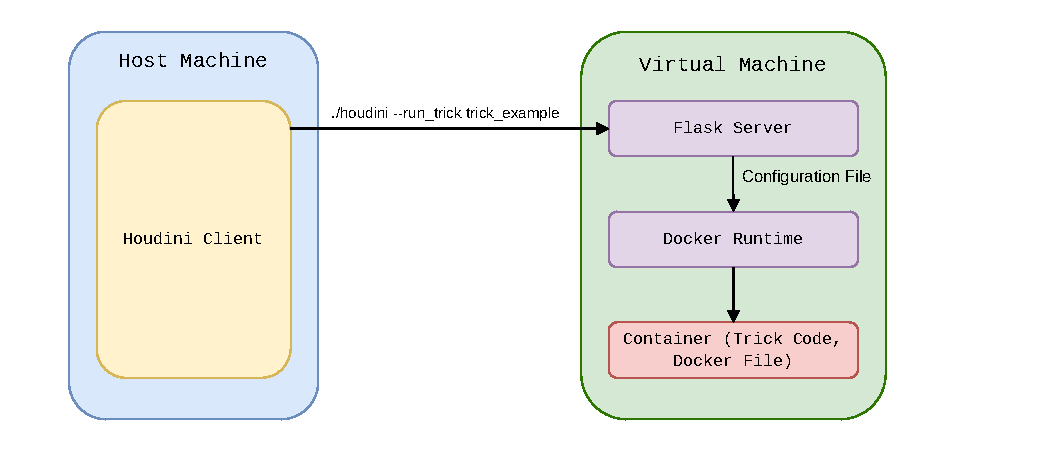
\includegraphics[width=1\linewidth]{figures/design.pdf}
  \caption{\DIFaddFL{Architecture of Houdini}}\label{fig:state-architecture}
\end{figure}

\section{\DIFadd{Reproducibility}}

\DIFadd{A central design goal of Houdini is to ensure that container security tests are reproducible, meaning that the same test, when run under the same conditions, will produce identical results regardless of when or where it is executed. Houdini achieves reproducibility through a combination of strict version control, deterministic execution environments, and isolation from external influences.
}

\DIFadd{Each test in Houdini runs inside a new VM that is freshly booted from a Buildroot-based }\DIFaddend image. This \DIFdelbegin \DIFdel{eliminates state sharing between tests and prevents contamination }\DIFdelend \DIFaddbegin \DIFadd{means that every test starts in a clean environment, with no leftover data or settings }\DIFaddend from previous runs. \DIFdelbegin \DIFdel{No background services, daemons, or user-modifiable system components are present in the guest image, further ensuring that results are solely attributable to the test configuration. Because no persistent state is carried between executions, the test environment is fully reset each time, enabling strict reproducibility and simplifying debugging. This design guarantees that the observed behavior reflects the actual impact of the container configuration under test, free from side effects introduced by prior tests or host-level interactions.
}\DIFdelend \DIFaddbegin \DIFadd{As soon as a test finishes, the VM is thrown away, so nothing carries over into the next test. This helps make sure that results are consistent and not affected by what happened before.
}\DIFaddend 

\DIFdelbegin \section{\DIFdel{Version Pinning}}
%DIFAUXCMD
\addtocounter{section}{-1}%DIFAUXCMD
\DIFdelend \DIFaddbegin \DIFadd{The Buildroot image is very minimal, it only includes what’s absolutely needed to run the test. It doesn’t have background programs like update services, SSH, or scheduled tasks, which could introduce randomness or unexpected behavior. By keeping things simple and stripped down, Houdini ensures that the only things running in the VM are the ones the user specifically added for the test.
}

\DIFadd{This clean and predictable setup makes it much easier to get the same results every time a test is run. Even if a trick is repeated many times or on different machines, the outcome stays consistent because the environment is always the same.
}

\DIFadd{To avoid changes caused by updates or host system drift, Houdini uses a version pinning mechanism. Version pinning refers to the practice of explicitly specifying and using fixed versions of software components rather than relying on the latest or system-default versions. This ensures that tests always use the same binaries, regardless of when or where they are run, and prevents unexpected changes in behavior due to automatic updates or upstream changes. In the context of container security testing, version pinning is essential because even minor updates to Docker, runc, or the kernel can introduce subtle behavioral differences.
}\DIFaddend 

To ensure reproducibility\DIFdelbegin \DIFdel{and enable systematic regression testing}\DIFdelend , Houdini enforces strict control over the versions of all critical software components involved in test execution. \DIFaddbegin \DIFadd{Critical software components include the Linux kernel, Docker, and runc. }\DIFaddend Container behavior can change significantly between versions of \DIFdelbegin \DIFdel{Docker, runc, or the Linux kernel}\DIFdelend \DIFaddbegin \DIFadd{these tools}\DIFaddend , even when the container configuration \DIFdelbegin \DIFdel{itself }\DIFdelend remains unchanged. To eliminate variability caused by \DIFdelbegin \DIFdel{underlying }\DIFdelend software drift, Houdini \DIFdelbegin \DIFdel{relies on a }\DIFdelend \DIFaddbegin \DIFadd{adopts a comprehensive }\DIFaddend version pinning strategy\DIFdelbegin \DIFdel{that explicitly fixes the versions of all major runtime components}\DIFdelend .

Each test \DIFdelbegin \DIFdel{case specifies exact }\DIFdelend \DIFaddbegin \DIFadd{in Houdini explicitly declares the }\DIFaddend versions of Docker, runc, and the Linux kernel \DIFaddbegin \DIFadd{to be used}\DIFaddend . These components are \DIFdelbegin \DIFdel{precompiled }\DIFdelend \DIFaddbegin \DIFadd{downloaded from official release sources, precompiled, }\DIFaddend and stored in a \DIFdelbegin \DIFdel{local cache, ensuring }\DIFdelend \DIFaddbegin \DIFadd{structured local cache. This guarantees }\DIFaddend that the same binaries are \DIFdelbegin \DIFdel{used }\DIFdelend \DIFaddbegin \DIFadd{reused }\DIFaddend across repeated runs. For example, if a trick is \DIFdelbegin \DIFdel{meant }\DIFdelend \DIFaddbegin \DIFadd{intended }\DIFaddend to evaluate a vulnerability \DIFdelbegin \DIFdel{present }\DIFdelend in runc 1.0.0-rc2 but \DIFdelbegin \DIFdel{fixed }\DIFdelend \DIFaddbegin \DIFadd{verify its resolution }\DIFaddend in 1.1.12, Houdini \DIFdelbegin \DIFdel{will use the exact corresponding runc binary for each test case }\DIFdelend \DIFaddbegin \DIFadd{retrieves the exact binaries for each version and uses them directly, }\DIFaddend without relying on \DIFaddbegin \DIFadd{system }\DIFaddend package managers or \DIFdelbegin \DIFdel{internet downloads}\DIFdelend \DIFaddbegin \DIFadd{external internet access}\DIFaddend . Similarly, \DIFdelbegin \DIFdel{different versions of Docker (e.g., }\DIFdelend \DIFaddbegin \DIFadd{multiple Docker versions such as }\DIFaddend 20.10.3, 23.0.1, or 27.0.3 \DIFdelbegin \DIFdel{) }\DIFdelend can be tested \DIFdelbegin \DIFdel{across the same trick logic to assess behavioral driftor identify regressions}\DIFdelend \DIFaddbegin \DIFadd{against the same logic to study behavioral drift}\DIFaddend .

\DIFdelbegin \DIFdel{These precompiled binaries are injected into the guest VM using }\DIFdelend \DIFaddbegin \DIFadd{Houdini uses }\DIFaddend an overlay filesystem \DIFdelbegin \DIFdel{. Rather than }\DIFdelend \DIFaddbegin \DIFadd{to make testing both efficient and consistent. Instead of }\DIFaddend rebuilding the entire \DIFdelbegin \DIFdel{root filesystem for each test }\DIFdelend \DIFaddbegin \DIFadd{VM image from scratch for every test case, it starts with a common}\DIFaddend , \DIFdelbegin \DIFdel{Houdini layers the required binaries over the static Buildroot image. This technique allows different test cases to share a commonbase environment while customizing their runtime stack independently. Overlay injection ensures that the guest VM sees only the specified versions of the relevant tools, regardless of what is installed on the host.
}%DIFDELCMD < 

%DIFDELCMD < %%%
\DIFdel{The guest operating system itself is built using Buildroot, a minimalist Linux build system that allows fine-grained control over the contents of the root filesystem. Houdini uses Buildroot to construct deterministic VM images that contain only the essential componentsneeded for trick execution. This eliminates potential sources of nondeterminism that are common in general-purpose distributions}\DIFdelend \DIFaddbegin \DIFadd{precompiled base image generated using Buildroot. On top of this base, Houdini layers only the necessary test-specific components}\DIFaddend , such as \DIFdelbegin \DIFdel{automatic updates, dependency resolution, and unpredictable background services.
}%DIFDELCMD < 

%DIFDELCMD < %%%
\DIFdel{By combining precompiled runtime components, overlay injection, and deterministic Buildroot-generated VMs, Houdini creates a fully controlled execution environment. This infrastructure ensures that any changes in trick behavior can be confidently attributed to intentional differences in configuration or runtime version—not to hidden changes in the surrounding software stack. It also enables robust regression testing, where the same trick is executed across a range of versions to observe how security guarantees evolve over time. This approach was particularly useful in the evaluation of CVE-2024-21626, where Houdini revealed that the vulnerability was present in runc versions earlier than those initially reported in the official CVE disclosure}\DIFdelend \DIFaddbegin \DIFadd{particular versions of Docker, runc using an overlay. This means the same lightweight VM can be reused across multiple tests, while still ensuring that each test runs with precisely the versions of the tools it is supposed to evaluate. By isolating these versions from the host system, Houdini guarantees a controlled and repeatable testing environment regardless of changes on the host machine}\DIFaddend .


\section{\DIFdelbegin \DIFdel{Test Matrix Design}\DIFdelend \DIFaddbegin \DIFadd{Scalability}\DIFaddend }

Houdini is \DIFdelbegin \DIFdel{designed to support systematic and }\DIFdelend \DIFaddbegin \DIFadd{built to support }\DIFaddend large-scale container security \DIFdelbegin \DIFdel{testing through a declarative test matrix model. Instead of requiring users to write custom scripts for each test case, Houdini allows users to define a matrix of configuration options that are automatically expanded into individual test cases. This approach simplifies the process of specifying and managing complex experiments, reduces manual effort, and improves coverage across different isolation and privilege }\DIFdelend \DIFaddbegin \DIFadd{evaluations without requiring extensive manual effort or scripting. While each test is executed serially to maintain isolation and determinism, the overall framework is designed to scale efficiently across hundreds or thousands of test }\DIFaddend configurations.

\DIFdelbegin \DIFdel{Each trick execution is defined by a set of configuration "knobs" that control how the container is launched. These knobs include Linux capabilities (e.g. , }\texttt{\DIFdel{CAP\_SYS\_ADMIN}}%DIFAUXCMD
\DIFdelend \DIFaddbegin \DIFadd{At the core of Houdini’s scalability is its matrix-based testing model. Instead of manually defining each test case, users specify sets of options, such as Docker flags}\DIFaddend , \DIFdelbegin \texttt{\DIFdel{CAP\_SYS\_PTRACE}}%DIFAUXCMD
\DIFdel{), namespace modes (such as }\texttt{\DIFdel{--pid=host}} %DIFAUXCMD
\DIFdel{or }\texttt{\DIFdel{--net=host}}%DIFAUXCMD
\DIFdel{), AppArmor profiles (e.g., }\texttt{\DIFdel{unconfined}} %DIFAUXCMD
\DIFdel{or }\texttt{\DIFdel{docker-default}}%DIFAUXCMD
\DIFdel{), seccomp profiles, user identity (root vs. non-root), and Docker flagslike }\texttt{\DIFdel{--privileged}}%DIFAUXCMD
\DIFdel{, }\texttt{\DIFdel{--read-only}}%DIFAUXCMD
\DIFdel{, or volume mounts. Users specify the set of values they wish to test for each knob using a simple configuration format, typically YAML or JSON. }%DIFDELCMD < 

%DIFDELCMD < %%%
\DIFdel{Once specified, Houdini }\DIFdelend \DIFaddbegin \DIFadd{Linux capabilities, namespace settings, or user identities that they want to explore. Houdini then }\DIFaddend automatically generates the Cartesian product of \DIFdelbegin \DIFdel{all parameter combinations, pairing each with the target trick and runtime version. For example, if a user wants to test a single trick across 3 Docker versions, 2 AppArmor profiles, and 2 sets of capabilities, Houdini will automatically generate 12 distinct test cases(3 × 2 × 2), each representing a unique configuration. This process eliminates the need for manual duplication and ensures that all combinations are systematically evaluated}\DIFdelend \DIFaddbegin \DIFadd{these options, producing a comprehensive list of test cases. This allows for systematic evaluation of all meaningful combinations without the need for custom scripts or duplicated logic}\DIFaddend .

\DIFdelbegin \DIFdel{This declarative model significantly enhances scalability. Rather than managing each test manually, users can define broad sets of scenarios with a few lines of configuration. }\DIFdelend Houdini’s internal scheduler \DIFdelbegin \DIFdel{then handles the execution of each test case in a clean, isolated virtual machine, capturing results independently. This approach enables researchers to explore how different isolation settings interact, detect edge cases, and identify configurations that break expected security boundaries}\DIFdelend \DIFaddbegin \DIFadd{ensures that each test is executed in isolation within a clean virtual machine. It manages the lifecycle of each VM, booting, running the trick, capturing the output, and tearing down the environment, without user intervention. This automation allows large batches of tests to be run back-to-back, making it possible to evaluate broad security surfaces such as how different container configurations behave across Docker and runc versions, or how changes to namespace settings influence process visibility}\DIFaddend .

\DIFdelbegin \DIFdel{By abstracting test case specification into a declarative matrix, Houdini provides a scalable and maintainable framework for container security testing. It empowers users to conduct extensive coverage experiments with minimal manual configuration, while preserving precision and reproducibility in each individual test}\DIFdelend \DIFaddbegin \DIFadd{To handle high test volumes efficiently, Houdini optimizes performance through the reuse of lightweight Buildroot-based VM images and precompiled runtime binaries. It avoids rebuilding environments from scratch and instead layers test-specific components on top of a shared base image using an overlay filesystem. This not only saves time but also reduces system resource usage}\DIFaddend .


\section{\DIFaddbegin \DIFadd{Host }\DIFaddend Isolation\DIFdelbegin \DIFdel{and Safety Mechanisms}\DIFdelend }

Houdini is explicitly designed to safely execute potentially dangerous or privilege-escalating container workloads without risking the security or stability of the host system. \DIFdelbegin \DIFdel{To achieve this, it enforces strict isolation through a combination of virtual machine separation , containment policies, and runtime safeguards}\DIFdelend \DIFaddbegin \DIFadd{This is achieved through strict isolation enforced by running all tests inside QEMU-based virtual machines (VMs). This approach ensures strong separation between the test environment and the host, providing both safety and reproducibility}\DIFaddend .

\DIFdelbegin \DIFdel{All trick executions occur inside a QEMU-based virtual machine}\DIFdelend \DIFaddbegin \DIFadd{Each trick is executed within its own QEMU VM}\DIFaddend , which serves as a hardware-level \DIFdelbegin \DIFdel{boundary between the test environment and the host}\DIFdelend \DIFaddbegin \DIFadd{isolation boundary}\DIFaddend . Unlike approaches that rely \DIFdelbegin \DIFdel{on Linux containers alone}\DIFdelend \DIFaddbegin \DIFadd{solely on Linux container isolation}\DIFaddend , this VM-level \DIFdelbegin \DIFdel{separation }\DIFdelend \DIFaddbegin \DIFadd{sandbox }\DIFaddend guarantees that even if a container successfully \DIFdelbegin \DIFdel{breaks out of }\DIFdelend \DIFaddbegin \DIFadd{escapes }\DIFaddend its sandbox, it remains confined \DIFdelbegin \DIFdel{within the virtualized guest . This defense-in-depth model protects the host from both known and unknown container escape vulnerabilities, ensuring that test payloads cannot influence or damage the system running Houdini itself}\DIFdelend \DIFaddbegin \DIFadd{to the guest environment. No test payload can reach or affect the host operating system, making Houdini suitable for executing untrusted or potentially malicious code safely}\DIFaddend .

Houdini further avoids any direct linkage between the host and the guest environment. No host directories are mounted into the guest, and no namespaces are shared between the host and VM. Containers are launched entirely within the guest’s user, mount, PID, and network namespaces. \DIFdelbegin \DIFdel{This means that }\DIFdelend \DIFaddbegin \DIFadd{As a result, }\DIFaddend containers inside the VM have no visibility into host processes, filesystems, or resources. \DIFdelbegin \DIFdel{Features }\DIFdelend \DIFaddbegin \DIFadd{Flags }\DIFaddend such as \texttt{--pid=host} only apply within the \DIFdelbegin \DIFdel{context of the VM , and never bridge to the real host}\DIFdelend \DIFaddbegin \DIFadd{VM context and never expose the physical host-level information}\DIFaddend .

\DIFdelbegin \DIFdel{To empirically verify that host access is not possible, Houdiniincorporates a canary mechanism. During VM boot, a simulated host-accessible path is defined }\DIFdelend \DIFaddbegin \DIFadd{Houdini’s reliance on QEMU offers several key advantages over alternative virtualization platforms such as VMware or VirtualBox. First, QEMU supports both full system emulation and hardware-assisted virtualization through KVM, allowing it to run unmodified Linux kernels and minimalist userland environments generated by Buildroot. It can boot directly from a raw kernel image }\DIFaddend (e.g., \DIFdelbegin \DIFdel{a file or directory that mimics a mounted host volume) . The trick under test may attempt to write to this path or read from it as part of the test logic. If the container can successfully access this canary, it indicates a misconfiguration or a potential escape vector. In practice, Houdini’s isolation model prevents such access unless the VM itself has been misconfigured, providing an additional layer of runtime validation.
}%DIFDELCMD < 

%DIFDELCMD < %%%
\DIFdel{Together, these mechanisms enforce strong host isolation and make Houdini a safe platform for evaluating security-critical container behavior. By containing tests within a tightly scoped virtual environment, it ensures that no trick—malicious or accidental—can compromise the integrity of the host system.
}%DIFDELCMD < 

%DIFDELCMD < %%%
\section{\DIFdel{Motivation for Virtualized Execution}}
%DIFAUXCMD
\addtocounter{section}{-1}%DIFAUXCMD
%DIFDELCMD < 

%DIFDELCMD < %%%
\DIFdel{A central architectural decision in Houdini is to execute all container tests inside a lightweight virtual machine, rather than directly on the host system. This approach is primarily motivated by the need for environmental control, cross-system reproducibility, and kernel-level flexibility.
}%DIFDELCMD < 

%DIFDELCMD < %%%
\DIFdel{First, running inside a VM ensures a **clean and deterministic environment**. Houdini uses a minimal Buildroot-based Linux system as its virtualized testbed, which eliminates the variability and complexity commonly found in general-purpose operating systems. This avoids interference from background services, user-installed software, or automatic updates, thereby reducing noise in test outcomes and ensuring that any observed behavior is solely due to the container configuration under test }\DIFdelend \DIFaddbegin \texttt{\DIFadd{bzImage}}\DIFadd{) without requiring a bootloader or full OS, enabling precise control over the testing environment}\DIFaddend .

Second, \DIFdelbegin \DIFdel{virtualization enables **reproducibility across different machines and over time**. Because the virtual machine is booted from a fixed kernel image and root filesystem, the entire runtime environment remains identical regardless of the underlying host. This makes it possible to compare results across test runs and systems with confidence, knowing that the execution context has not drifted. Such consistency is essential for empirically validating container security guarantees, especially when fine-grained differences in runtime behavior may influence security outcomes}\DIFdelend \DIFaddbegin \DIFadd{QEMU supports complete command-line configuration, including CPU model, memory size, disk images, network interfaces, and serial ports. This makes it ideal for automated and reproducible test workflows. In contrast, VMware and VirtualBox rely on graphical interfaces and more static configurations, which hinder automation and scripting}\DIFaddend .

Third, \DIFdelbegin \DIFdel{the virtual machine setup grants Houdini the ability to **precisely control the kernel version** used during testing. This is a key capability for evaluating the evolution of confinement mechanisms across different Linux releases. Houdini can boot any custom or historical kernel version without modifying the host system, enabling security researchers to assess whether a given trick succeeds or fails as a function of kernel changes alone. This capability is essential for regression testing and understanding the security implications of kernel-level patches and configuration options. }%DIFDELCMD < 

%DIFDELCMD < %%%
\DIFdel{Together, these properties make VM-based execution a foundational component of Houdini’s design, enabling systematic, consistent, and historically-aware container security testing. }%DIFDELCMD < 

%DIFDELCMD < %%%
\section{\DIFdel{Automation and Execution Pipeline}}
%DIFAUXCMD
\addtocounter{section}{-1}%DIFAUXCMD
%DIFDELCMD < 

%DIFDELCMD < %%%
\DIFdel{Houdini is designed to operate as a fully automated and repeatable test execution framework. Once a user specifies the desired trick and configuration matrix, the system takes over and handles all stages of test orchestration without requiring further manual intervention. This fully unattended execution pipeline reduces the user burden and enables large-scale evaluations to proceed with minimal effort.
}%DIFDELCMD < 

%DIFDELCMD < %%%
\DIFdel{Each test case is executed in isolation within its own QEMU virtual machine. The VMs are launched one at a time in a serialized fashion—Houdini does not currently support parallel execution. While this limits overall throughput, it offers a crucial benefit: predictability. Serial execution ensures that each test runs in a clean environment free from interference by other tasks, removing concurrency as a source of nondeterminism.
}%DIFDELCMD < 

%DIFDELCMD < %%%
\DIFdel{To enforce repeatability, Houdini initializes a fresh VM for every single test case. The guest image is regenerated using a minimal Buildroot system, and no state from previous runs is carried over. This guarantees that the environment is identical each time a trick is executed. Whether running a test for the first time or rerunning it weeks later with the same configuration, the outcome will be determined solely by the logic of the trick and the versions of the software under test—not by stale filesystem state, cached data, or unpredictable side effects. }%DIFDELCMD < 

%DIFDELCMD < %%%
\DIFdel{This strict separation and automation pipeline allow users to queue hundreds or thousands of test cases and walk away, confident that results will be recorded consistently and reliably. Logs are saved automatically, configuration metadata is attached to every result, and errors are surfaced clearly for debugging. In effect, Houdini abstracts away the operational complexity of container security testing, allowing researchers and engineers to focus on analysis rather than setup and execution}\DIFdelend \DIFaddbegin \DIFadd{QEMU is architecture-agnostic. It supports x86, ARM, MIPS, RISC-V, and other architectures, allowing for cross-platform testing. While Houdini currently focuses on x86\_64, the use of QEMU ensures that it can easily be extended to other architectures in the future. VMware and VirtualBox are limited to x86-based virtualization and do not support full system emulation for other CPU architectures}\DIFaddend .


\section{Transparency and Debuggability}

Houdini is designed not only to execute tests reliably, but also to make results easy to interpret and debug. To support transparency and effective diagnosis, the framework implements structured logging \DIFdelbegin \DIFdel{, rich metadata tagging, and deterministic evaluation criteria }\DIFdelend for every test.

Each test execution generates a structured log file that includes the container's standard output, standard error, exit code, and a timestamped record of the configuration parameters used. These logs are stored in a standardized format and organized by test ID, making it straightforward to trace the provenance of any result. Whether a trick passed, failed, or encountered an unexpected runtime error, the corresponding log provides clear visibility into what occurred during execution.

Houdini also tags every test result with its full configuration metadata. This includes the container runtime version, kernel version, Docker flags, capabilities, namespace modes, and any AppArmor or seccomp profiles in effect. These tags are recorded alongside the test result, enabling automated analysis, filtering, and regression tracking. For example, a user can easily compare how the same trick behaves under different runc versions or with different namespace settings, based on the metadata attached to each result.

\DIFdelbegin \DIFdel{While the default mode is fully automated, Houdini also supports optional interactive inspection. Users can choose to pause execution at specific stages, such as before launching the container or after the trick completes. This allows them to manually inspect the state of the VM or container, check file system contents, or rerun the trick interactively for more detailed debugging.
}%DIFDELCMD < 

%DIFDELCMD < %%%
\DIFdel{Finally, each trick is written to emit a deterministic pass or fail outcome based on runtime observations. For instance, a trick might check for the presence of a specific file, the ability to signal another process, or the success of a privilege escalation attempt. These conditions are embedded in the trick logic itself, ensuring that the result of each test is consistent and reproducible across runs. By combining clear pass/fail semantics with detailed logs and metadata, Houdini provides a transparent and developer-friendly environment for security evaluation.
}%DIFDELCMD < 

%DIFDELCMD < %%%
\section{\DIFdel{Security Design}}
%DIFAUXCMD
\addtocounter{section}{-1}%DIFAUXCMD
%DIFDELCMD < 

%DIFDELCMD < %%%
\DIFdel{A central aspect of Houdini's architecture is its emphasis on safe execution of potentially harmful container workloads. The primary security boundary is enforced at the level of a QEMU virtual machine, which isolates each test from the host system using hardware-level virtualization. This boundary is sufficient for Houdini’s threat model, which assumes that container workloads may attempt to exploit kernel vulnerabilities or escalate privileges within the guest. By design, no test has direct access to the host’s filesystem, namespaces, or process tree. Even if a trick succeeds in breaking out of its container, it only reaches the VM environment, which is ephemeral and isolated. Furthermore, no host-mounted volumes or devices are exposed to the guest, and Houdini does not rely on nested virtualization or host-provided namespaces. This model ensures that trick execution remains safely contained, protecting both the host and other tests from compromise.
}%DIFDELCMD < 

%DIFDELCMD < %%%
\section{\DIFdel{Extensibility}}
%DIFAUXCMD
\addtocounter{section}{-1}%DIFAUXCMD
%DIFDELCMD < 

%DIFDELCMD < %%%
\DIFdel{Houdini is designed to be modular and extensible, allowing security researchers to easily add new tricks, runtimes, or configuration parameters. Each trick is defined by a set of modular files: a Dockerfile, a configuration file, and a script. Adding a new trick simply requires placing these files in a new subdirectory and registering the trick in the Houdini CLI. Similarly, new runtime versions—such as a different version of Docker, runc, or the Linux kernel—can be added to Houdini’s local cache, after which they become available as selectable options in the test matrix. While the current implementation focuses on Docker and runc, the system is structured in a way that would allow integration of other OCI-compliant runtimes like }\texttt{\DIFdel{crun}} %DIFAUXCMD
\DIFdel{or }\texttt{\DIFdel{youki}} %DIFAUXCMD
\DIFdel{with relatively few changes. This modularity ensures that Houdini can evolve alongside the container ecosystem and be used to evaluate future attack surfaces or isolation strategies with minimal developer effort.
}%DIFDELCMD < 

%DIFDELCMD < %%%
\section{\DIFdel{Buildroot Customization and Guest Environment Design}}
%DIFAUXCMD
\addtocounter{section}{-1}%DIFAUXCMD
%DIFDELCMD < 

%DIFDELCMD < %%%
\DIFdel{Houdini's guest virtual machine is built using Buildroot, a minimalist embedded Linux build system that allows tight control over the software included in the image. This customization is critical for maintaining determinism, minimizing attack surface, and reducing boot time. The Buildroot image includes only the essential components required for container execution and trick evaluation. These include a statically linked BusyBox shell, the Docker daemon and CLI (injected via overlay), a Python interpreter, curl for HTTP communication, and a lightweight init system. 
}%DIFDELCMD < 

%DIFDELCMD < %%%
\DIFdel{Deliberate trade-offs are made to exclude non-essential services such as SSH, udev, systemd, or networking daemons, which could introduce nondeterministic behavior or additional complexity. Instead, the VM is initialized with a fixed set of devices and predictable kernel logs, enabling stable trick execution. Statically linking utilities where possible simplifies debugging by avoiding dynamic library mismatches and dependency issues across test runs. The result is a clean, lightweight VM that boots quickly and behaves identically across repeated invocations, serving as a robust platform for empirical security testing.
}%DIFDELCMD < 

%DIFDELCMD < %%%
\section{\DIFdel{Error Handling and Recovery}}
%DIFAUXCMD
\addtocounter{section}{-1}%DIFAUXCMD
%DIFDELCMD < 

%DIFDELCMD < %%%
\DIFdel{Houdini includes built-in mechanisms to detect and handle failures at each stage of test execution. If a VM fails to boot within a predefined timeout, the test is automatically marked as failed and the error is logged with a timestamp and diagnostic message. Similarly, if Docker fails to start inside the guest—due to misconfiguration, missing binaries, or runtime incompatibilities—the failure is detected by the trick listener and reported back to the host as an infrastructure-level error.
}%DIFDELCMD < 

%DIFDELCMD < %%%
\DIFdel{If the trick script itself crashes or exits unexpectedly, Houdini captures the exit code, standard output, and standard error of the container process. These artifacts are stored in structured logs, allowing users to distinguish between trick-level failures and broader environment issues. For non-critical errors such as missing config fields or malformed input, Houdini logs a warning and skips execution of the invalid test case. In all cases, error metadata is retained alongside test results for later review.
}%DIFDELCMD < 

%DIFDELCMD < %%%
\DIFdel{Although Houdini does not currently support automatic retries, its deterministic and stateless design makes re-running failed cases straightforward. Users can selectively rerun individual test IDs using the CLI, ensuring minimal overhead when diagnosing flakiness or debugging regressions.
}%DIFDELCMD < 

%DIFDELCMD < %%%
\section{\DIFdel{Configuration Validation and Sanity Checks}}
%DIFAUXCMD
\addtocounter{section}{-1}%DIFAUXCMD
%DIFDELCMD < 

%DIFDELCMD < %%%
\DIFdel{Before executing any test, Houdini performs a series of pre-run validation checks to ensure the integrity and completeness of the user-provided configuration. These include verifying that all required trick files are present (configuration file, Dockerfile, and script), that the specified Docker and runc versions exist in the local binary cache, and that configuration parameters such as capability names, AppArmor profiles, and namespace flags are syntactically valid.
}%DIFDELCMD < 

%DIFDELCMD < %%%
\DIFdel{The CLI also checks for duplicate or conflicting configurations, such as attempting to run a test with both }\texttt{\DIFdel{--privileged}} %DIFAUXCMD
\DIFdel{and a restricted seccomp profile. If such conflicts are detected, the system emits a warning and skips the invalid case. Users are also warned if required components (e.g., QEMU, KVM, or Buildroot toolchain) are not installed or misconfigured on the host system.
}%DIFDELCMD < 

%DIFDELCMD < %%%
\DIFdel{These validation steps are critical for preventing wasted test runs, simplifying troubleshooting, and maintaining the integrity of large-scale evaluations. By catching errors early in the pipeline, Houdini ensures that only well-formed and meaningful test cases are executed.
}%DIFDELCMD < 

%DIFDELCMD < %%%
\section{\DIFdel{Interface and User Experience Design}}
%DIFAUXCMD
\addtocounter{section}{-1}%DIFAUXCMD
%DIFDELCMD < 

%DIFDELCMD < %%%
\DIFdel{Houdini provides a command-line interface (CLI) as its primary mode of interaction. The CLI is designed to balance flexibility with usability, allowing both simple and advanced users to manage trick execution workflows efficiently. Common commands include }\texttt{\DIFdel{houdini run}} %DIFAUXCMD
\DIFdel{to execute a trick, }\texttt{\DIFdel{houdini matrix}} %DIFAUXCMD
\DIFdel{to expand a configuration file into concrete test cases, and }\texttt{\DIFdel{houdini rerun}} %DIFAUXCMD
\DIFdel{to re-execute failed or inconclusive tests by test ID. Each command provides contextual feedback, including progress indicators, error summaries, and log file locations.
}%DIFDELCMD < 

%DIFDELCMD < %%%
\DIFdel{The experiment configuration itself is defined declaratively using a YAML-based format that is human-readable and easy to edit. Users can specify default settings at the global level and override them for individual test cases as needed. This model reduces redundancy and simplifies management of large matrices. 
}%DIFDELCMD < 

%DIFDELCMD < %%%
\DIFdel{Test results are presented in a structured, color-coded table that highlights pass/fail status, runtime versions, and key configuration flags. Logs are accessible by test ID and organized in a predictable directory structure, allowing quick navigation and review. Overall, Houdini’s interface is designed to support transparency, traceability, and low-friction experimentation for researchers and engineers.
}%DIFDELCMD < 

%DIFDELCMD < %%%
\section{\DIFdel{Runtime Injection via OverlayFS}}
%DIFAUXCMD
\addtocounter{section}{-1}%DIFAUXCMD
%DIFDELCMD < 

%DIFDELCMD < %%%
\DIFdel{Rather than relying on Buildroot’s package infrastructure to download and install Docker and runc inside the VM, we used an overlayfs directory to inject precompiled binaries of both components directly into the root filesystem. This approach provides full control over the runtime environment and ensures that only explicitly specified versions are used during testing. We chose not to use Buildroot packages because doing so introduced limitations: several historical versions of Docker and runc were either unavailable or failed to build consistently within Buildroot’s package ecosystem. By manually sourcing and verifying the binaries, we were able to include a broader range of versions and maintain compatibility across all tests.
}%DIFDELCMD < 

%DIFDELCMD < %%%
\section{\DIFdel{Preventing Environmental Drift}}
%DIFAUXCMD
\addtocounter{section}{-1}%DIFAUXCMD
%DIFDELCMD < 

%DIFDELCMD < %%%
\DIFdel{Environmental drift refers to unintentional changes in the system that can affect the outcome of container-based tests. These changes may include automatic updates to the operating system, differences in kernel versions, updated system libraries, or changes in container runtime behavior. Even when a test script remains the same, such background variation can cause container behavior to differ between runs, leading to inconsistent or misleading results.
}%DIFDELCMD < 

%DIFDELCMD < %%%
\DIFdel{This is a critical concern for security testing, where consistency is essential. Without environmental stability, researchers may encounter false positives, where a trick appears to succeed because of an incidental change, or false negatives, where a real vulnerability is masked by a system-level patch or configuration shift. In either case, the test results become untrustworthy, and any security claims based on those results may be invalid.
}%DIFDELCMD < 

%DIFDELCMD < %%%
\DIFdel{To address this, Houdini is designed to eliminate sources of environmental drift by creating a fully version-controlled, deterministic testing environment. All critical components that influence container behavior, including the Linux kernel, Docker engine, and runc runtime are manually sourced, precompiled, and injected into the root filesystem using an overlay filesystem. This ensures that Houdini uses only explicitly specified versions of each component, independent of host updates or package manager behavior.
}%DIFDELCMD < 

%DIFDELCMD < %%%
\DIFdel{This design choice was necessary because many historical versions of Docker and runc are either unavailable through Buildroot’s package system or fail to build due to missing dependencies or upstream changes. By bypassing the package infrastructure and directly injecting verified binaries, Houdini achieves a consistent and reproducible runtime environment across all test sessions.
}%DIFDELCMD < 

%DIFDELCMD < %%%
\DIFdel{Additionally, Houdini uses Buildroot to generate a minimal, static guest operating system that excludes background services, update agents, or untracked dependencies that could introduce nondeterminism. The virtual machine is launched without networking to prevent environmental noise from DNS, package mirrors, or remote services. Only a single, tightly scoped communication channel is exposed to the host through a QEMU user-mode forwarded port used for reporting results.
}%DIFDELCMD < 

%DIFDELCMD < %%%
\DIFdel{Together, these design decisions ensure that Houdini provides a frozen, deterministic environment where test outcomes are reproducible over time. This stability is especially important for longitudinal analysis, vulnerability tracking, patch verification, and reproducible research, where changes in the results must reflect actual differences in the tested logic, not unintended changes in the surrounding system.
}%DIFDELCMD < 

%DIFDELCMD < %%%
\section{\DIFdel{Support for Custom Kernels}}
%DIFAUXCMD
\addtocounter{section}{-1}%DIFAUXCMD
%DIFDELCMD < 

%DIFDELCMD < %%%
\DIFdel{Houdini supports the use of custom Linux kernel builds, enabling researchers to evaluate container behavior on non-standard or experimental kernels. This is particularly useful for testing scenarios that require kernel features not available in mainline releases, or for reproducing issues on distribution-specific kernels.
}%DIFDELCMD < 

%DIFDELCMD < %%%
\DIFdel{Users can specify a custom kernel image (bzImage) to be used when launching the QEMU virtual machine. Instead of selecting a precompiled kernel from Houdini’s internal cache, the user provides a path to an externally built kernel through the CLI or configuration file. Houdini will boot the VM with this specified kernel while keeping the rest of the guest environment unchanged.
}%DIFDELCMD < 

%DIFDELCMD < %%%
\DIFdel{This feature allows full control over the kernel used during testing, including:
}%DIFDELCMD < 

%DIFDELCMD < %%%
\DIFdel{Custom-compiled kernels with modified configuration options.
}%DIFDELCMD < 

%DIFDELCMD < %%%
\DIFdel{Vendor-patched or downstream distribution kernels.
}%DIFDELCMD < 

%DIFDELCMD < %%%
\DIFdel{Legacy kernels for historical reproduction.
}%DIFDELCMD < 

%DIFDELCMD < %%%
\DIFdel{The guest root filesystem, Docker engine, and runc version remain consistent regardless of the selected kernel, ensuring that observed behavior differences are attributable solely to the kernel in use. This modularity supports high-fidelity experimentation without altering the test orchestration pipeline.
}%DIFDELCMD < 

%DIFDELCMD < %%%
\DIFdel{To preserve safety, custom kernels are still booted inside isolated QEMU virtual machines. This ensures that even if the custom kernel is unstable or includes regressions, it cannot affect the host system.
}%DIFDELCMD < 

%DIFDELCMD < %%%
\DIFdel{This flexibility makes Houdini a valuable platform for kernel-centric container security research, where testing across a range of kernel versions and configurations is essential.
}%DIFDELCMD < 

%DIFDELCMD < %%%
\section{\DIFdel{Multi-Runtime Support}}
%DIFAUXCMD
\addtocounter{section}{-1}%DIFAUXCMD
%DIFDELCMD < 

%DIFDELCMD < %%%
\DIFdel{Houdini is designed to support multiple container runtimes, recognizing that the behavior of container isolation features may vary significantly between runtime implementations. While Docker commonly defaults to }\texttt{\DIFdel{runc}}%DIFAUXCMD
\DIFdel{, the Open Container Initiative (OCI) standard permits alternative runtimes that comply with the OCI runtime specification. To ensure comprehensive testing coverage and enable comparisons across runtimes, Houdini includes support for both }\texttt{\DIFdel{runc}} %DIFAUXCMD
\DIFdel{and }\texttt{\DIFdel{crun}}%DIFAUXCMD
\DIFdel{, with a modular design that facilitates the integration of additional runtimes in the future.
}%DIFDELCMD < 

%DIFDELCMD < %%%
\DIFdel{Each runtime is precompiled and stored in Houdini’s local binary cache, just like Docker and kernel versions. When executing a test, Houdini injects the selected runtime into the guest virtual machine using its overlay filesystem. The trick configuration specifies the desired runtime, and Houdini ensures that only the corresponding binary is present in the guest environment during test execution. This guarantees that observed behavior reflects the exact runtime under test and is not influenced by any system defaults.
}%DIFDELCMD < 

%DIFDELCMD < %%%
\DIFdel{The current implementation includes support for }\texttt{\DIFdel{runc}}%DIFAUXCMD
\DIFdel{, the default Docker runtime, and }\texttt{\DIFdel{crun}}%DIFAUXCMD
\DIFdel{, a high-performance alternative developed by the Open Container Initiative. These runtimes can be swapped per test case, allowing users to evaluate how different runtime implementations handle security boundaries such as capabilities, seccomp profiles, or namespace interactions.
}%DIFDELCMD < 

%DIFDELCMD < %%%
\DIFdel{The runtime selection is fully configurable via Houdini’s YAML and Python-based configuration models. In matrix mode, users can easily define a list of runtimes to test, and Houdini will generate test cases across all specified versions. For example, users can observe how a trick behaves when executed under both }\texttt{\DIFdel{runc}} %DIFAUXCMD
\DIFdel{and }\texttt{\DIFdel{crun}}%DIFAUXCMD
\DIFdel{, using the same container image, kernel version, and security flags.
}%DIFDELCMD < 

%DIFDELCMD < %%%
\DIFdel{The system is structured to allow the addition of other OCI-compliant runtimes, such as }\texttt{\DIFdel{youki}} %DIFAUXCMD
\DIFdel{or }\texttt{\DIFdel{Kata Containers}}%DIFAUXCMD
\DIFdel{, with minimal changes. New runtimes can be added to the local cache and referenced in trick configurations just like existing ones. This extensibility ensures that Houdini remains adaptable to changes in the container runtime landscape and can be used to validate the correctness and security of emerging runtime implementations.
}%DIFDELCMD < 

%DIFDELCMD < %%%
\DIFdel{By supporting multiple runtimes, Houdini empowers researchers to perform comparative analysis, detect behavioral regressions, and evaluate implementation differences that may affect container confinement. This capability is critical for ensuring that container security claims hold consistently across the diverse and evolving set of OCI runtimes.
}%DIFDELCMD < 

%DIFDELCMD < %%%
\section{\DIFdel{Limitations}}
%DIFAUXCMD
\addtocounter{section}{-1}%DIFAUXCMD
%DIFDELCMD < 

%DIFDELCMD < %%%
\DIFdel{While Houdini offers a robust foundation for reproducible container security testing, it currently has several limitations. First, it does not support parallel execution; tests are run sequentially to guarantee isolation and avoid concurrency-related nondeterminism. This serialized execution model simplifies debugging and analysis but can be a bottleneck for very large-scale evaluations. Second, Houdini’s runtime support is presently limited to Docker and runc. While the system is extensible, it does not yet include out-of-the-box support for other runtimes like }\texttt{\DIFdel{crun}} %DIFAUXCMD
\DIFdel{or }\texttt{\DIFdel{youki}}%DIFAUXCMD
\DIFdel{, which limits its coverage of the broader container landscape. Finally, Houdini assumes a Linux-based host system with QEMU and KVM support, which may restrict portability to some environments such as macOS or Windows. These limitations represent areas for future development as the framework matures.
}%DIFDELCMD < 

%DIFDELCMD < %%%
\DIFdelend \end{doublespace} 	\fontsize{12pt}{14pt} \selectfont
\begin{doublespace}
\chapter{Implementation}


\section{Trick Structure Overview}

Houdini supports two primary modes for defining and executing tricks. The first is a YAML-based approach where a single trick is fully specified through a standalone configuration file. This method is ideal for running individual tests with carefully controlled settings, making it well-suited for targeted investigations or manual debugging. The second mode is a Python-based approach that allows users to define parameter sets as lists, which Houdini expands into a Cartesian product to form a complete test matrix. For example, parameters can be defined in Python, and Houdini will automatically generate all combinations to be tested.



\section{YAML-Based Trick Definition}

Each trick in Houdini is composed of three modular components that work together to define and execute a container-based security test: a configuration file, a trick script, and a Dockerfile. The configuration file is a YAML document that specifies the parameters for launching the Docker container, including security-related settings such as Linux capabilities, namespace modes, AppArmor profiles, user privileges, and resource limits. These parameters are parsed by Houdini and translated directly into Docker API calls, ensuring that containers are created with precise, repeatable configurations.

The second component is the trick script, which contains the logic of the test and is executed inside the container. Typically written in Python or Bash, this script attempts a specific action—such as reading a sensitive file, sending a signal to a process, or escalating privileges—and reports the outcome by printing a success or failure message. The semantics of what constitutes a pass or fail are entirely defined by the script, giving users full control over evaluation criteria.

The final component is the Dockerfile, which builds the container image and defines the runtime environment. It includes instructions for copying the trick script into the container, installing any necessary dependencies, and specifying the base image to use. This modular architecture allows each component to be modified independently.

This YAML-based approach is ideal for running single, isolated experiments with controlled configurations, making it especially useful for debugging, demonstration, or documentation purposes.

\section{Configuration File}

Each Houdini trick begins with a configuration file, written in YAML styled format, that defines the runtime parameters used to launch the container. This file acts as the source of truth for how the container is constructed and executed. It specifies a range of Docker options including Linux capabilities (via \texttt{cap\_add} and \texttt{cap\_drop}), namespace settings (such as \texttt{pid\_mode} and \texttt{userns\_mode}), resource limits (e.g., \texttt{cpu\_shares}, \texttt{mem\_limit}), volume mounts, user identity, and security options such as AppArmor profiles or seccomp settings.

The configuration is declarative and follows a structured YAML schema that maps directly to Docker’s low-level run options. For example, if a user wants to disable privilege escalation, enable a read-only filesystem, or run the container as a non-root user with dropped capabilities, these settings can be encoded clearly in the configuration file. This abstraction allows users to focus on the security scenario being tested without needing to handcraft long and error-prone Docker command-line arguments.

When Houdini executes a test, the CLI parses the YAML configuration and validates it before test execution begins. It checks for required fields, ensures that runtime versions and trick paths are valid, and performs consistency checks to catch errors like incompatible or conflicting flags. Once validated, the configuration is sent to the virtual machine through the host’s Flask server, where it is interpreted by the trick listener and translated into a Docker run command within the guest environment.

This structured approach ensures consistency and transparency. Since all configurations are encoded in a machine-readable format and logged alongside test results, they can be reproduced exactly in future runs or used as part of larger matrix-based experiments. It also supports modularity: the same configuration file can be reused across different tricks, or slightly modified to explore alternative isolation boundaries.

Below is an example of a configuration file used in Houdini. It defines a container with default Docker isolation settings and specifies the Dockerfile and trick path:

\begin{figure}[H]
\caption{Configuration file for a default Docker out-of-the-box security setting.}
\label{fig:configuration-file}
\begin{lstlisting}[caption={}, numbers=left, numberstyle=\tiny, stepnumber=1, breaklines=true, frame=single, backgroundcolor=\color{gray!10}, basicstyle=\ttfamily\scriptsize, showspaces=false, showstringspaces=false]
name: out-of-the-box docker configuration
dockerfile:
  - path: Dockerfile
dependencies:
  - server: False
docker_config: 
  - network_mode: bridge
  - read_only: False
  - security_opt: []
  - pid_mode: null
  - cpu_shares: 1024
  - volumes : []
  - mem_limit: null
  - cpuset_cpus: null
  - cpu_quota: null
  - cpu_period: null
  - cap_add: []
  - cap_drop: []
  - privileged: False
  - user: root
  - pids_limit: null
  - ipc_mode: private
  - userns_mode: null
trick:
  - path: /houdini/tricks/OutOfTheBoxExample
\end{lstlisting}
\end{figure}




\section{Trick Script}

The trick script is the core component that defines the actual security test logic to be executed inside the container. This script is typically written in a high-level language such as Python or Bash and is copied into the container during the build process specified by the Dockerfile. Once the container is launched with the desired configuration, the trick script runs automatically and attempts a specific action, such as reading a sensitive file, accessing a kernel interface, or interacting with another process. Its purpose is to evaluate whether the container configuration enforces the intended security boundaries.

Houdini does not impose restrictions on the scripting language used, though Python and Bash are most commonly employed due to their simplicity and compatibility with minimal container environments. The scripting interface is straightforward: the script performs a predefined action and prints a result indicating whether the trick passed or failed. These results are captured via standard output by the trick listener running inside the guest virtual machine. The listener uses these outputs, along with exit codes and standard error messages, to classify the outcome of the test.

The evaluation criteria are entirely defined within the trick script, giving users full control over what constitutes success or failure. This flexibility allows Houdini to support a wide range of test types, from low-level privilege checks to higher-level behavioral verifications. Scripts can also emit additional diagnostic messages to aid in debugging or deeper analysis.

Below is an example of a simple Python trick script that tests whether the container is able to read the contents of the \texttt{/etc/shadow} file. Under standard Docker security settings, access to this file should be restricted. If the script is able to read it, the trick is considered to have passed—indicating a misconfiguration or insufficient isolation. Otherwise, it fails.

\begin{figure}[H]
\caption{Example trick implementation that checks for read access to \texttt{/etc/shadow}.}
\label{fig:trick-script}
\begin{lstlisting}[language=Python, numbers=left, numberstyle=\tiny, stepnumber=1, breaklines=true, frame=single, backgroundcolor=\color{gray!10}, basicstyle=\ttfamily\scriptsize, showspaces=false, showstringspaces=false]
import os

def check_shadow_access():
    path = "/etc/shadow"
    if os.path.exists(path):
        try:
            with open(path, 'r') as f:
                print("Able to read /etc/shadow:")
                print("Trick passed")
        except PermissionError:
            print("Permission denied to read /etc/shadow.")
            print("Trick failed")
        except Exception as e:
            print(f"Unexpected error: {e}")
            print("Trick failed")
    else:
        print("/etc/shadow does not exist.")
        print("Trick failed")

check_shadow_access()
\end{lstlisting}
\end{figure}


This example demonstrates how a trick can evaluate a specific security assumption—file access control in this case—and produce a deterministic result that Houdini can log and interpret. More advanced tricks may incorporate conditionals, environment checks, or IPC mechanisms, but the basic structure remains the same: run a check and report a pass/fail outcome in a clear and reproducible manner.



\section{Dockerfile}

The Dockerfile is responsible for setting up the container's runtime environment so that the trick script can execute reliably and with all necessary dependencies. It defines how the container image is built, including the selection of a base image, the installation of packages or libraries required by the trick script, and the inclusion of the trick file itself.

Tricks in Houdini can be written in a variety of languages such as Python or Bash, so the Dockerfile must ensure that the corresponding runtime (e.g., the Python interpreter or Bash shell) is available inside the container. This often involves installing system packages using the package manager provided by the base image—for example, using \texttt{apt} in Debian-based images or \texttt{apk} in Alpine.

Another essential part of the Dockerfile is copying the trick script into the container's filesystem. This step ensures that the logic defined by the user is available at a known path when the container starts. Houdini standardizes this by copying the trick to a predefined directory (e.g., \texttt{/houdini/trick.py}) so that all containers follow the same execution convention.

The base image is selected based on the needs of the trick. Lightweight images like Alpine Linux are often preferred for simple tests because of their small size and fast startup time. However, more feature-rich images like Debian or Python-based official images may be used when additional dependencies or language runtimes are required.

Finally, the Dockerfile specifies an entrypoint or \texttt{CMD} directive to automatically run the trick script when the container launches. This ensures that the trick executes without requiring user intervention or manual commands. The entrypoint is usually a direct call to the interpreter (e.g., \texttt{python3 /houdini/trick.py}) or a shell script that wraps additional logic.

The example below demonstrates a simple Dockerfile used in Houdini to run a Python-based trick. It uses the official Python image, copies the trick into the container, and sets the default command to execute the script:

\begin{figure}[H]
\caption{Example Dockerfile used to prepare the container environment for a Python-based trick.}
\label{fig:dockerfile-example}
\begin{lstlisting}[numbers=left, numberstyle=\tiny, stepnumber=1, breaklines=true, frame=single, backgroundcolor=\color{gray!10}, basicstyle=\ttfamily\scriptsize, showspaces=false, showstringspaces=false]
FROM python:3.9-slim

WORKDIR /houdini

COPY trick.py /houdini/trick.py

CMD ["python3", "/houdini/trick.py"]
\end{lstlisting}
\end{figure}


This Dockerfile is minimal yet sufficient for running Python scripts inside a container. It illustrates the typical pattern used in Houdini to prepare containers in a consistent and reproducible manner. More complex tricks may extend this file to install additional packages, configure environment variables, or mount external resources, but the core structure remains largely the same.


\section{Python-Based Parameter Expansion Mode}

In addition to supporting single-trick YAML definitions, Houdini provides a Python-based mechanism to define a matrix of configurations by specifying parameters as lists. Houdini automatically expands these parameters into a Cartesian product and generates a full suite of test cases. This approach is powerful for scaling up experiments, allowing researchers to explore the interaction of various container runtime settings systematically.

\begin{lstlisting}[language=bash, caption={Trick parameter sets defined in Python}, label={lst:apparmor-trick}, numbers=left, numberstyle=\tiny, stepnumber=1, breaklines=true, frame=single, backgroundcolor=\color{gray!10}, basicstyle=\ttfamily\footnotesize, showspaces=false, showstringspaces=false]
pid_mode = [None, "--pid=host"]
cap_kill = [False, True]
cap_sys_ptrace = [False, True]
privileged_opts = [False, True]
apparmor_profiles = ["apparmor=unconfined", "apparmor=docker-default"]
user = ["huzi"]
runtime = ["crun"]
\end{lstlisting}

Let $\mathcal{P}$ denote the parameter space. We define:

\[
\begin{aligned}
\mathcal{P}_{\text{pid}} &= \{\varnothing, \texttt{"--pid=host"}\} \\
\mathcal{P}_{\text{kill}} &= \{\texttt{False}, \texttt{True}\} \\
\mathcal{P}_{\text{ptrace}} &= \{\texttt{False}, \texttt{True}\} \\
\mathcal{P}_{\text{priv}} &= \{\texttt{False}, \texttt{True}\} \\
\mathcal{P}_{\text{apparmor}} &= \{\texttt{"apparmor=unconfined"}, \texttt{"apparmor=docker-default"}\} \\
\mathcal{P}_{\text{user}} &= \{\texttt{"huzi"}\} \\
\mathcal{P}_{\text{runtime}} &= \{\texttt{"crun"}\}
\end{aligned}
\]

The full parameter space is their Cartesian product:

\[
\mathcal{P} = \mathcal{P}_{\text{pid}} \times \mathcal{P}_{\text{kill}} \times \mathcal{P}_{\text{ptrace}} \times \mathcal{P}_{\text{priv}} \times \mathcal{P}_{\text{apparmor}} \times \mathcal{P}_{\text{user}} \times \mathcal{P}_{\text{runtime}}
\]

Each tuple $\vec{p} \in \mathcal{P}$ corresponds to a single command invocation:

\[
\texttt{docker run -i } + \text{flags}(\vec{p}) + \texttt{ \$IMAGE}
\]

Since \(|\mathcal{P}_{\text{pid}}| = |\mathcal{P}_{\text{kill}}| = |\mathcal{P}_{\text{ptrace}}| = |\mathcal{P}_{\text{priv}}| = |\mathcal{P}_{\text{apparmor}}| = 2\) and \(|\mathcal{P}_{\text{user}}| = |\mathcal{P}_{\text{runtime}}| = 1\), the total number of configurations is:

\[
|\mathcal{P}| = 2^5 = 32
\]

\noindent Below are the 32 commands generated by iterating over all elements in $\mathcal{P}$:

\begin{lstlisting}[language=bash, caption={Generated Docker run commands from Cartesian expansion}, label={lst:docker-combinations}, numbers=left, numberstyle=\tiny, stepnumber=1, breaklines=true, frame=single, backgroundcolor=\color{gray!10}, basicstyle=\ttfamily\tiny, showspaces=false, showstringspaces=false]
docker run -i --user huzi --security-opt apparmor=unconfined --runtime crun $IMAGE
docker run -i --user huzi --security-opt apparmor=unconfined --cap-add CAP_KILL --runtime crun $IMAGE
docker run -i --user huzi --security-opt apparmor=unconfined --cap-add CAP_SYS_PTRACE --runtime crun $IMAGE
docker run -i --user huzi --security-opt apparmor=unconfined --cap-add CAP_KILL --cap-add CAP_SYS_PTRACE --runtime crun $IMAGE
docker run -i --user huzi --security-opt apparmor=unconfined --privileged --runtime crun $IMAGE
docker run -i --user huzi --security-opt apparmor=unconfined --privileged --cap-add CAP_KILL --runtime crun $IMAGE
docker run -i --user huzi --security-opt apparmor=unconfined --privileged --cap-add CAP_SYS_PTRACE --runtime crun $IMAGE
docker run -i --user huzi --security-opt apparmor=unconfined --privileged --cap-add CAP_KILL --cap-add CAP_SYS_PTRACE --runtime crun $IMAGE
docker run -i --user huzi --security-opt apparmor=docker-default --runtime crun $IMAGE
docker run -i --user huzi --security-opt apparmor=docker-default --cap-add CAP_KILL --runtime crun $IMAGE
docker run -i --user huzi --security-opt apparmor=docker-default --cap-add CAP_SYS_PTRACE --runtime crun $IMAGE
docker run -i --user huzi --security-opt apparmor=docker-default --cap-add CAP_KILL --cap-add CAP_SYS_PTRACE --runtime crun $IMAGE
docker run -i --user huzi --security-opt apparmor=docker-default --privileged --runtime crun $IMAGE
docker run -i --user huzi --security-opt apparmor=docker-default --privileged --cap-add CAP_KILL --runtime crun $IMAGE
docker run -i --user huzi --security-opt apparmor=docker-default --privileged --cap-add CAP_SYS_PTRACE --runtime crun $IMAGE
docker run -i --user huzi --security-opt apparmor=docker-default --privileged --cap-add CAP_KILL --cap-add CAP_SYS_PTRACE --runtime crun $IMAGE
docker run -i --user huzi --pid=host --security-opt apparmor=unconfined --runtime crun $IMAGE
docker run -i --user huzi --pid=host --security-opt apparmor=unconfined --cap-add CAP_KILL --runtime crun $IMAGE
docker run -i --user huzi --pid=host --security-opt apparmor=unconfined --cap-add CAP_SYS_PTRACE --runtime crun $IMAGE
docker run -i --user huzi --pid=host --security-opt apparmor=unconfined --cap-add CAP_KILL --cap-add CAP_SYS_PTRACE --runtime crun $IMAGE
docker run -i --user huzi --pid=host --security-opt apparmor=unconfined --privileged --runtime crun $IMAGE
docker run -i --user huzi --pid=host --security-opt apparmor=unconfined --privileged --cap-add CAP_KILL --runtime crun $IMAGE
docker run -i --user huzi --pid=host --security-opt apparmor=unconfined --privileged --cap-add CAP_SYS_PTRACE --runtime crun $IMAGE
docker run -i --user huzi --pid=host --security-opt apparmor=unconfined --privileged --cap-add CAP_KILL --cap-add CAP_SYS_PTRACE --runtime crun $IMAGE
docker run -i --user huzi --pid=host --security-opt apparmor=docker-default --runtime crun $IMAGE
docker run -i --user huzi --pid=host --security-opt apparmor=docker-default --cap-add CAP_KILL --runtime crun $IMAGE
docker run -i --user huzi --pid=host --security-opt apparmor=docker-default --cap-add CAP_SYS_PTRACE --runtime crun $IMAGE
docker run -i --user huzi --pid=host --security-opt apparmor=docker-default --cap-add CAP_KILL --cap-add CAP_SYS_PTRACE --runtime crun $IMAGE
docker run -i --user huzi --pid=host --security-opt apparmor=docker-default --privileged --runtime crun $IMAGE
docker run -i --user huzi --pid=host --security-opt apparmor=docker-default --privileged --cap-add CAP_KILL --runtime crun $IMAGE
docker run -i --user huzi --pid=host --security-opt apparmor=docker-default --privileged --cap-add CAP_SYS_PTRACE --runtime crun $IMAGE
docker run -i --user huzi --pid=host --security-opt apparmor=docker-default --privileged --cap-add CAP_KILL --cap-add CAP_SYS_PTRACE --runtime crun $IMAGE
\end{lstlisting}




\section{Execution Pipeline}

Houdini’s execution pipeline is designed to take a user-defined trick and run it in a fully controlled and reproducible environment. The process begins on the host system, where the user selects a trick and provides its associated configuration, either through a YAML file or a Python-based matrix. Houdini’s command-line interface (CLI) parses this configuration, verifies its correctness, and prepares the test case for execution. Validation includes checking that required files exist, runtime versions are available in the local cache, and parameters such as capabilities and namespace modes are syntactically valid and logically consistent.

Once the configuration is validated, Houdini launches a new QEMU virtual machine using a Buildroot-generated image as the guest operating system. This virtual machine provides strong isolation, ensuring that even if a trick contains malicious logic or exploits a container escape vulnerability, the impact remains confined to the VM. During boot, the guest VM connects to a lightweight Flask server running on the host. This server acts as the communication bridge between the host and guest environments, exposing a simple HTTP API for transferring configuration data and receiving test results.

After the guest VM is online and connected, the Flask server sends the configuration for the trick to a persistent background service inside the VM known as the trick listener. This listener is responsible for setting up and executing the test within the guest. It begins by building the Docker image using the provided Dockerfile, copying the trick script into the container, and applying all specified configuration options such as capabilities, AppArmor profiles, and user identity.

Once the image is built, the container is launched with the defined Docker run settings. The trick script runs automatically inside the container, performing its test logic and writing its output to standard output and error streams. The trick listener monitors the container’s execution, capturing the exit code, output, and any diagnostic messages produced by the trick. These results are packaged together with the configuration metadata and returned to the host via the Flask server.

On the host side, Houdini stores all test results in structured logs indexed by test ID. This log includes the full configuration, trick output, container exit status, and timestamped metadata, making it easy to trace, compare, and debug results. The entire pipeline—from configuration parsing to result capture—is designed to run without manual intervention, enabling users to queue and evaluate large sets of tests in a reliable and repeatable manner.

By combining strict virtual machine isolation, automated container orchestration, and lightweight communication via Flask, Houdini provides a robust and secure pipeline for container security testing that is both scalable and transparent.


\section{Example Trick: Shadow File Access}

To demonstrate Houdini’s end-to-end workflow, a simple example trick is provided that attempts to access the \texttt{/etc/shadow} file from inside a container. This trick is not an exploit, but rather a baseline check designed to verify that basic file system isolation is functioning correctly under the container’s security configuration. The motivation for this test lies in the sensitivity of the \texttt{/etc/shadow} file, which stores hashed system passwords and should only be accessible to privileged processes. Under standard Docker configurations, containers should be unable to read this file unless they are overly privileged or misconfigured.

The expected behavior, when Docker is running in its default configuration, is that access to \texttt{/etc/shadow} will be denied. The container process should either encounter a permission error or be unable to open the file at all. This trick validates that Docker’s default isolation mechanisms—such as user identity mapping, read-only mounts, and AppArmor policies—are effective in preventing unauthorized access to host-sensitive files.

From a security evaluation perspective, this test serves as a sanity check. It allows users to confirm that their Houdini setup is working correctly and that the baseline container environment enforces expected isolation boundaries. If this simple trick unexpectedly passes, it indicates a serious misconfiguration that could invalidate the results of more complex security tests. As such, this example is often used as an initial test when setting up Houdini on a new host or validating a new kernel or Docker runtime version.

The full implementation of the trick script is provided in Listing~\ref{fig:trick-script}, and the corresponding container configuration is shown in Listing~\ref{fig:configuration-file}. When executed inside a container, the script attempts to open and read \texttt{/etc/shadow}. If it succeeds, it prints “Trick passed”; otherwise, it prints “Trick failed.” These results are captured and logged by Houdini as part of the standard execution pipeline. This example highlights the modularity and transparency of Houdini’s trick-based testing model and illustrates how a simple action can validate critical isolation guarantees.


\section{Flask Server Integration}

The Flask server plays a central role in Houdini’s architecture by acting as the primary communication bridge between the host system and the guest virtual machine. Once the QEMU-based Buildroot VM boots, it establishes a connection to this Flask server to initiate trick execution, request runtime metadata, or receive configuration files. The server runs as a lightweight HTTP service on the host, exposing a set of well-defined endpoints that orchestrate the full test workflow.

Among the core endpoints exposed by the server are \texttt{/run-trick}, \texttt{/run-command-in-vm}, and \texttt{/server-status}. The \texttt{/server-status} endpoint is used for health checking and indicates whether the Houdini server is actively running on the host. This is implemented by checking for the Python process associated with the server:

\begin{lstlisting}[language=python, caption={Server health check endpoint}, label={lst:server-status}, numbers=left, numberstyle=\tiny, stepnumber=1, breaklines=true, frame=single, backgroundcolor=\color{gray!10}, basicstyle=\ttfamily\footnotesize, showspaces=false, showstringspaces=false]
@app.route('/server-status', methods=['GET'])
def server_status():
    if is_service_running('/usr/bin/python3 /houdini/server.py'):
        response_data = str(True)
        return make_response(response_data, 200)
    else:
        response_data = str(False)
        return make_response(response_data, 503)
\end{lstlisting}

The \texttt{/version-status} endpoint queries the current versions of critical components such as Docker and \texttt{runc}. It executes shell commands using Python’s \texttt{subprocess} module and returns a JSON-formatted response with version information:

\begin{lstlisting}[language=python, caption={Runtime version information endpoint}, label={lst:version-status}, numbers=left, numberstyle=\tiny, stepnumber=1, breaklines=true, frame=single, backgroundcolor=\color{gray!10}, basicstyle=\ttfamily\footnotesize, showspaces=false, showstringspaces=false]
@app.route('/version-status', methods=['GET'])
def version_status():
    versions = get_versions()
    return make_response(jsonify(versions), 200)
\end{lstlisting}

The most critical endpoint, \texttt{/run-trick}, handles the dispatching of a specific trick into the guest VM. When a request is made to this endpoint, the server loads the corresponding YAML configuration file, parses it, and executes the full Docker test pipeline. Output is captured using an in-memory stream to allow full logging of results:

\begin{lstlisting}[language=python, caption={Trick execution endpoint}, label={lst:run-trick}, numbers=left, numberstyle=\tiny, stepnumber=1, breaklines=true, frame=single, backgroundcolor=\color{gray!10}, basicstyle=\ttfamily\footnotesize, showspaces=false, showstringspaces=false]
@app.route('/run-trick/<trick_folder>/<trick>', methods=['GET'])
def run_trick(trick_folder, trick):
    TRICK_PATH = f'/houdini/tricks/{trick_folder}/{trick}'
    if not os.path.exists(TRICK_PATH):
        return jsonify({'error': f'Trick {trick} not found. PATH = {TRICK_PATH}'}), 404

    with open(TRICK_PATH, 'r') as file:
        trick_data = yaml.safe_load(file)

    output = io.StringIO()
    with contextlib.redirect_stdout(output):
        results = parse_trick_and_run(trick_data, request.args)

    return Response(output.getvalue())
\end{lstlisting}

For debugging and exploratory testing, the \texttt{/run-command-in-vm} endpoint allows arbitrary shell commands to be executed within the VM environment. This is particularly useful for checking environment settings or container state without needing a full trick configuration:

\begin{lstlisting}[language=python, caption={Run shell command in VM}, label={lst:run-command}, numbers=left, numberstyle=\tiny, stepnumber=1, breaklines=true, frame=single, backgroundcolor=\color{gray!10}, basicstyle=\ttfamily\footnotesize, showspaces=false, showstringspaces=false]
@app.route('/run-command-in-vm', methods=['GET'])
def run_command_in_vm():
    cmd = request.args.get('cmd')
    try:
        output_lines = []
        with subprocess.Popen(
            cmd, shell=True, stdout=subprocess.PIPE, stderr=subprocess.STDOUT, text=True
        ) as process:
            for line in process.stdout:
                output_lines.append(line)
        return jsonify({'output': ''.join(output_lines)})
    except Exception as e:
        return jsonify({'error': str(e)}), 500
\end{lstlisting}

Together, these endpoints enable seamless interaction between the host and guest systems. They allow Houdini to manage test execution in a modular, scriptable, and reproducible manner. The server abstracts complex Docker interactions and version management behind a simple HTTP API, making it easy to integrate into larger security testing workflows.


\section{Trick Listener and Trick Execution Logic}

The trick listener is a persistent background service running inside the QEMU virtual machine. Its role is to receive trick configurations sent from the host's Flask server and execute them in a controlled, containerized environment. At the heart of this execution logic lies the \texttt{parse\_trick\_and\_run()} function, which interprets the YAML trick configuration, builds the Docker image, launches the container with specified settings, and monitors the test.

The execution begins by parsing the YAML configuration file received via HTTP. This file is expected to contain two main sections: the \texttt{docker\_config} array and the \texttt{trick} dictionary. The configuration is validated to ensure all required fields exist, and the container name is extracted from the query string arguments.

The first step is to ensure any container from a previous run does not interfere. If a container with the same name is already running, it is forcefully terminated and removed:

\begin{lstlisting}[language=python, caption={Container cleanup}, label={lst:cleanup-container}, numbers=left, numberstyle=\tiny, stepnumber=1, breaklines=true, frame=single, backgroundcolor=\color{gray!10}, basicstyle=\ttfamily\footnotesize, showspaces=false, showstringspaces=false]
def check_if_container_is_running(container_name):
    try:
        existing_container = client.containers.get(container_name)
        print(f"Container {container_name} already exists. Removing it.")
        if existing_container.status == 'running':
            existing_container.kill(signal=SIGKILL)
        existing_container.remove(force=True)
    except docker.errors.NotFound:
        print(f"No existing container named {container_name} found.")
\end{lstlisting}

Next, the Docker image is built from the provided trick directory. This includes copying the Dockerfile and trick script into the working context. The image is tagged using the test name to ensure clear tracking:

\begin{lstlisting}[language=python, caption={Docker image build step}, label={lst:docker-build}, numbers=left, numberstyle=\tiny, stepnumber=1, breaklines=true, frame=single, backgroundcolor=\color{gray!10}, basicstyle=\ttfamily\footnotesize, showspaces=false, showstringspaces=false]
def build_docker_image(dockerfile_path, image_name):
    print("Creating Docker Image")
    client.images.build(path=".", tag=image_name, rm=True)
    print(f"Image '{image_name}' built successfully.")
\end{lstlisting}

Once built, the container is launched with the exact parameters specified in the configuration. These include capabilities, AppArmor, PID namespace settings, memory constraints, and more. Houdini uses the Docker SDK to pass these options directly to \texttt{client.containers.run()}:

\begin{lstlisting}[language=python, caption={Container launch logic}, label={lst:container-run}, numbers=left, numberstyle=\tiny, stepnumber=1, breaklines=true, frame=single, backgroundcolor=\color{gray!10}, basicstyle=\ttfamily\footnotesize, showspaces=false, showstringspaces=false]
container = client.containers.run(
    image=image_name,
    name=container_name,
    detach=True,
    network_mode=network_mode,
    read_only=read_only,
    security_opt=security_opt,
    pid_mode=pid_mode,
    cpu_shares=cpu_shares,
    volumes=volumes,
    mem_limit=mem_limit,
    cpuset_cpus=cpuset_cpus,
    cpu_quota=cpu_quota,
    cpu_period=cpu_period,
    cap_add=cap_add,
    cap_drop=cap_drop,
    privileged=privileged,
    user=user,
    pids_limit=pids_limit,
    ipc_mode=ipc_mode,
    userns_mode=userns_mode,
    stdout=True,
    stderr=True,
    tty=True,
)
\end{lstlisting}

Houdini then monitors the execution of the container, capturing the full stdout stream using \texttt{attach()} and waiting for the process to terminate. Once the container exits, its status code is recorded to determine if the trick passed, failed, or encountered an error:

\begin{lstlisting}[language=python, caption={Container monitoring and result capture}, label={lst:monitor-output}, numbers=left, numberstyle=\tiny, stepnumber=1, breaklines=true, frame=single, backgroundcolor=\color{gray!10}, basicstyle=\ttfamily\footnotesize, showspaces=false, showstringspaces=false]
for chunk in codecs.iterdecode(container.attach(stdout=True, stream=True), "utf-8"):
    sys.stdout.write(chunk)

exit_status = container.wait()
exit_code = exit_status['StatusCode']
print(f"Container exited with code: {exit_code}")
\end{lstlisting}

The results—comprising the container’s output, exit code, and execution metadata—are returned back to the Flask server, which then forwards them to the user via an HTTP response. This modular pipeline allows complete decoupling between test specification, execution, and result retrieval.

\vspace{1em}
\noindent
A simplified pseudocode version of \texttt{parse\_trick\_and\_run()} is shown below for clarity:

\begin{lstlisting}[language=python, caption={Pseudocode for Trick Execution}, label={lst:pseudocode-parse-trick}, numbers=left, numberstyle=\tiny, stepnumber=1, breaklines=true, frame=single, backgroundcolor=\color{gray!10}, basicstyle=\ttfamily\footnotesize, showspaces=false, showstringspaces=false]
def parse_trick_and_run(trick_data, args):
    container_name = args.get('container_name')
    check_if_container_is_running(container_name)
    build_docker_image(trick_data['trick'][0]['path'], container_name)
    container = run_docker_container(...all config params...)
    monitor_and_capture(container)
\end{lstlisting}

This function glues together every step in Houdini's lifecycle: it prepares the Docker image, applies the container runtime configuration, executes the trick, and forwards the result. Its simplicity belies the modular complexity and flexibility of Houdini’s test infrastructure.


\section{Version Reporting Endpoint}

To ensure complete reproducibility and traceability of test results, Houdini exposes a dedicated endpoint called \texttt{/version-status}. This endpoint provides runtime versioning information about critical components involved in container execution: Docker, \texttt{runc}, and \texttt{docker-runc}. These version numbers are essential for researchers to accurately interpret results and replicate experiments across systems with different host configurations.

When a request is made to \texttt{/version-status}, the Flask server calls a utility function named \texttt{get\_versions()}. This function executes shell commands using Python's \texttt{subprocess.check\_output()} to retrieve version strings from each runtime binary. It gracefully handles errors such as missing binaries or unexpected output formats, returning a JSON object with version strings or fallback messages.

The current implementation supports Docker, \texttt{runc}, and \texttt{docker-runc}, but can be extended to include kernel versions or other runtime environments. By returning this information as part of the test log, Houdini guarantees that every trick result is linked to a precise system state, supporting accurate debugging and longitudinal analysis.

Below is the code that implements this endpoint:

\begin{lstlisting}[language=python, caption={Version reporting logic for /version-status}, label={lst:version-status}, numbers=left, numberstyle=\tiny, stepnumber=1, breaklines=true, frame=single, backgroundcolor=\color{gray!10}, basicstyle=\ttfamily\footnotesize, showspaces=false, showstringspaces=false]
@app.route('/version-status', methods=['GET'])
def version_status():
    versions = get_versions()
    return make_response(jsonify(versions), 200)

def get_versions():
    versions = {}

    try:
        docker_output = subprocess.check_output(["docker", "--version"], stderr=subprocess.STDOUT)
        versions['docker'] = docker_output.decode().strip()
    except subprocess.CalledProcessError as e:
        versions['docker'] = f"Error: {e.output.decode().strip()}"
    except FileNotFoundError:
        versions['docker'] = "Docker not found"

    try:
        runc_output = subprocess.check_output(["runc", "--version"], stderr=subprocess.STDOUT)
        versions['runc'] = runc_output.decode().strip()
    except subprocess.CalledProcessError as e:
        versions['runc'] = f"Error: {e.output.decode().strip()}"
    except FileNotFoundError:
        versions['runc'] = "runc not found"

    try:
        docker_runc_output = subprocess.check_output(["docker-runc", "--version"], stderr=subprocess.STDOUT)
        versions['docker-runc'] = docker_runc_output.decode().strip()
    except subprocess.CalledProcessError as e:
        versions['docker-runc'] = f"Error: {e.output.decode().strip()}"
    except FileNotFoundError:
        versions['docker-runc'] = "docker-runc not found"

    return versions
\end{lstlisting}

This mechanism supports Houdini’s goal of rigorous reproducibility by anchoring trick results to specific software states. Extending this logic to include kernel version detection—by invoking \texttt{uname -r}—would further improve the system’s ability to document host-level conditions that influence container behavior.



\section{Dynamic Runtime Dispatch}

Houdini supports dynamic selection of container runtimes—specifically \texttt{runc} and \texttt{crun}—through both YAML-based trick definitions and Python-based test matrix expansions. This flexibility allows researchers to evaluate how different low-level runtimes handle the same security configurations, offering deeper insight into runtime-specific behavior.

Runtime selection is user-configurable in two ways. First, for YAML-defined tricks, the \texttt{runtime} field can be set explicitly (e.g., \texttt{crun}, \texttt{runc}) in the \texttt{docker\_config} section. Second, in matrix-driven experiments, runtime is one of the test parameters expanded using Cartesian product logic. A list of runtimes is defined in the configuration module and passed into the combination generator:

\begin{lstlisting}[language=python, caption={Runtime as a configurable test parameter in matrix mode}, label={lst:runtime-param}]
runtime = ["runc", "crun"]
...
def generate_combinations(config):
    fields = [
        ...
        config.get("runtime") or [None]
    ]
    return list(itertools.product(*fields))[:MAX_TESTS]
\end{lstlisting}

At runtime, the selected container runtime binary (e.g., \texttt{crun}) is injected into the guest virtual machine (QEMU) by copying the appropriate executable into the Buildroot overlay directory \texttt{/usr/bin} before VM boot. This is done dynamically based on the version set in \texttt{houdini\_config.py}. The correct binary is fetched from a pre-extracted folder of supported runtime versions:

\begin{lstlisting}[language=bash, caption={Injecting crun into the Buildroot overlay}, label={lst:get-crun}]
get_crun_binaries() {
    ...
    src_crun=$(find "$extracted_folder" -type f -name "crun-*linux-amd64" | head -n 1)
    cp "$src_crun" "${overlay_bin}/crun"
    chmod +x "${overlay_bin}/crun"
}
\end{lstlisting}

The Docker run command issued inside the VM includes the \texttt{--runtime} flag if a runtime is specified. This enables Houdini to test container behavior across multiple OCI runtimes within a uniform framework:

\begin{lstlisting}[language=python, caption={Runtime applied during container launch}, label={lst:runtime-docker-run}]
if isinstance(runtime, str):
    cmd += ["--runtime", str(runtime)]
\end{lstlisting}

This modular dispatch mechanism is designed for future extensibility. Support for additional runtimes such as \texttt{youki}, \texttt{Kata Containers}, or \texttt{gVisor} can be added by extending the binary injection logic and updating the configuration schema to recognize new runtime identifiers.

By making the container runtime a first-class configurable dimension in experiments, Houdini enables nuanced differential testing that can expose inconsistencies, vulnerabilities, or behavioral discrepancies across runtime implementations.


\section{Trick Parameter Expansion Logic}

Houdini supports large-scale, automated testing through its ability to expand parameterized test configurations into a full matrix of trick executions. This is achieved by defining each configuration parameter as a list—such as \texttt{pid\_mode}, \texttt{cap\_sys\_ptrace}, or \texttt{user}—and computing the Cartesian product across all parameters. Each unique combination forms one specific instance of a trick to be tested.

Internally, Houdini loads these parameters from Python modules corresponding to the selected trick. Using Python’s \texttt{importlib}, it dynamically loads the values from each variable into a unified configuration dictionary. Parameters not explicitly defined default to a single-item list with a \texttt{None} value to ensure uniformity during expansion.

To generate the matrix, Houdini uses Python’s \texttt{itertools.product()} to compute the Cartesian product across all lists. This approach is simple, efficient, and scales well to a moderate number of parameters. Each combination is then passed into a container execution function that builds the necessary Docker run command for that configuration.

To limit runtime and avoid combinatorial explosion, Houdini caps the number of generated tests using the \texttt{MAX\_TESTS} constant, which discards excess combinations if the matrix size becomes too large. This trade-off maintains a balance between thoroughness and execution feasibility.

Below is a simplified pseudocode version of the expansion and execution logic, taken from Houdini’s core driver script:

\begin{lstlisting}[language=python, caption={Generating and iterating over parameter combinations}, label={lst:matrix-expansion}, numbers=left, numberstyle=\tiny, stepnumber=1, breaklines=true, frame=single, backgroundcolor=\color{gray!10}, basicstyle=\ttfamily\footnotesize, showspaces=false, showstringspaces=false]
def load_config(trick_name):
    config_module = importlib.import_module(f"{trick_name}")
    config = {}
    for var in ["pid_mode", "cap_kill", "cap_sys_ptrace", 
                "privileged_opts", "apparmor_profiles", "user",  
                "net_bind_service", "cap_drop_all", "runtime"]:
        config[var] = getattr(config_module, var, [None])
    return config

def generate_combinations(config):
    fields = [
        config.get("pid_mode"),
        config.get("cap_kill"),
        config.get("cap_sys_ptrace"),
        config.get("privileged_opts"),
        config.get("apparmor_profiles"),
        config.get("user"),
        config.get("net_bind_service"),
        config.get("cap_drop_all"),
        config.get("runtime")
    ]
    return list(itertools.product(*fields))[:MAX_TESTS]
\end{lstlisting}

This design enables Houdini to efficiently run comprehensive test suites with varying parameters across container runtimes, user identities, namespace modes, and Linux capabilities. It also supports extensibility, as new parameters can be added to the configuration without altering the underlying expansion logic.


\section{Security Considerations in Host-Level Code}

Houdini is designed to execute potentially dangerous container configurations and scripts in a safe and reproducible environment. To ensure host system integrity, Houdini carefully separates test execution from the host by sandboxing all container activity within a QEMU virtual machine. This isolation guarantees that even if a containerized trick exploits a misconfiguration or escapes the container runtime, it remains confined within the guest VM, protecting the host from compromise. For this reason, all subprocess executions—including Docker image builds, container runs, and file access tests—are offloaded to the VM environment.

This design decision also ensures that Houdini's host-side Python code does not directly interact with untrusted trick scripts or configurations. By shifting the attack surface into the VM, Houdini minimizes privilege exposure and keeps the host clean of any temporary state or Docker containers created during testing.

Another key consideration is Docker Hub's rate limiting policy. Without authentication, anonymous users are restricted to a limited number of image pulls and builds per six-hour window. To avoid encountering these rate limits during large-scale test execution, Houdini requires authenticated Docker access using a personal access token. This is handled in the host logic via a login step:

\begin{lstlisting}[language=python, caption={Logging into Docker Hub to bypass image build limits}, label={lst:docker-login}, numbers=left, numberstyle=\tiny, stepnumber=1, breaklines=true, frame=single, backgroundcolor=\color{gray!10}, basicstyle=\ttfamily\footnotesize, showspaces=false, showstringspaces=false]
username = os.getenv("DOCKER_USERNAME")
password = os.getenv("DOCKER_TOKEN")
client = docker.from_env()
client.login(username=username, password=password)
\end{lstlisting}

This login process ensures that authenticated API calls to Docker Hub are used when building and pulling images. It also allows users with Docker Pro or Team subscriptions to take advantage of higher rate limits and private repository access.

\section{Virtual Machine Setup and Execution}

Houdini runs all container-based security tests inside a QEMU virtual machine to ensure strong host isolation and reproducibility. Each virtual machine is spun up dynamically for every trick, booting into a minimal Linux distribution generated by Buildroot. This architecture isolates all container behavior from the host operating system and allows precise control over the kernel and filesystem.

\subsection{Purpose of Virtualization}

The use of virtualization provides several key benefits:
\begin{itemize}
\item \textbf{Security Isolation:} Containers cannot directly affect the host system, even if misconfigured or compromised.
\item \textbf{Reproducibility:} A consistent environment is provided for every test, removing host system variability.
\item \textbf{Custom Kernel Support:} Researchers can test custom kernel builds or apply experimental patches without rebooting the host.
\end{itemize}

\subsection{QEMU Execution Command}

Houdini uses QEMU to run a VM with a custom kernel and root filesystem. The Python method responsible for starting the virtual machine is shown below:

\begin{lstlisting}[language=python, caption={Python method to start the QEMU VM in Houdini}, label={lst:start-vm}, numbers=left, numberstyle=\tiny, stepnumber=1, breaklines=true, frame=single, backgroundcolor=\color{gray!10}, basicstyle=\ttfamily\footnotesize, showspaces=false, showstringspaces=false]
def start_vm(self, kernel=get_absolute_path(f"/kernels/{KERNEL_VERSION}/arch/x86/boot/bzImage"), drive=get_absolute_path("/buildroot/output/images/rootfs.ext2")):
qemu_cmd = [
"qemu-system-x86_64",
"-smp", str(CPU_CORES),
"-m", str(VM_RAM),
"-kernel", kernel,
"-drive", f"file={drive},if=virtio,format=raw",
"-append", "apparmor=1 security=apparmor rootwait root=/dev/vda console=tty1 console=ttyS0 loglevel=0 cgroup_enable=cpuset cgroup_enable=memory",
"-serial", "mon:stdio",
"-net", "nic,model=virtio",
"-net", f"user,hostfwd=tcp::{PORT}-:{PORT}",
"-nographic",
"-virtfs", "local,path=/home/huzi/Desktop,mount_tag=hostshare,security_model=mapped-file,id=hostshare"
]
\end{lstlisting}

\subsection{Key VM Configuration Options}

The following options in the QEMU command are critical to Houdini's testing workflow:

\begin{itemize}
\item \texttt{-kernel}: Loads a specific Linux kernel, enabling experiments across kernel versions or with custom patches.
\item \texttt{-drive if=virtio}: Uses a virtio-backed root filesystem for fast disk access and compatibility with Buildroot images.
\item \texttt{-append}: Passes kernel boot parameters, including enabling AppArmor and cgroups for isolation enforcement.
\item \texttt{-serial mon:stdio}: Routes guest output to the host terminal for logging and debugging.
\item \texttt{-nographic}: Disables the graphical interface to simplify deployment and speed up boot time.
\item \texttt{-virtfs}: Mounts a host folder into the VM using Plan 9 FS, useful for accessing logs or artifacts.
\item \texttt{-net nic} and \texttt{-net user,hostfwd}: Sets up a virtual NIC and forwards a TCP port for communication between the host and guest (e.g., for Flask server requests).
\end{itemize}

\subsection{Lifecycle of a Virtual Machine}

Each trick triggers a complete VM lifecycle:
\begin{enumerate}
\item \textbf{Boot}: A QEMU virtual machine is started with the specified kernel and rootfs.
\item \textbf{Connect}: A Flask server on the host communicates with a Python service inside the VM.
\item \textbf{Execute}: The trick is executed inside the VM, typically via Docker, and output is captured.
\item \textbf{Shutdown}: The VM is destroyed after test execution, ensuring isolation between runs.
\end{enumerate}

This tightly controlled VM-based execution model is central to Houdini's reliability, safety, and reproducibility guarantees.

\end{doublespace} 	\fontsize{12pt}{14pt} \selectfont
\begin{doublespace}
\chapter{Evaluation}

To validate Houdini’s effectiveness as a container security testing framework, we designed a diverse set of evaluations that reflect its core goals: reproducibility, scalability, performance, isolation, extensibility, and robustness. These tests were conducted to ensure that Houdini performs consistently across various environments and use cases, while also remaining resilient to edge cases and user modifications.

We first assess reproducibility, a foundational principle of Houdini, by executing identical tests across machines with different hardware specifications. This verifies that test outcomes are not tied to the underlying system architecture. Additionally, we verify reproducibility over time by pinning the Docker, kernel, and runc versions and rerunning the same configurations after a delay. This demonstrates Houdini’s ability to deliver stable and consistent results, even as the underlying system evolves.

To evaluate scalability, we run a large batch of tricks \DIFdelbegin \DIFdel{—}\DIFdelend \DIFaddbegin \DIFadd{(}\DIFaddend up to 32\DIFdelbegin \DIFdel{—}\DIFdelend \DIFaddbegin \DIFadd{) }\DIFaddend across multiple configurations in a single session. This allows us to measure runtime, memory usage, and failure rates, \DIFdelbegin \DIFdel{offering }\DIFdelend \DIFaddbegin \DIFadd{which offers }\DIFaddend insight into Houdini’s performance under load. Complementing this, we conduct performance benchmarking by timing the full lifecycle of a trick, including \DIFdelbegin \DIFdel{virtual machine }\DIFdelend \DIFaddbegin \DIFadd{VM }\DIFaddend boot, container setup, and result capture. These times are compared against manual baseline executions to quantify Houdini’s overhead.

Host isolation is validated through a deliberately malicious trick designed to attempt writes to \DIFaddbegin \DIFadd{physical }\DIFaddend host-accessible paths. Success \DIFaddbegin \DIFadd{in this specific evaluation }\DIFaddend is defined by the inability of \DIFdelbegin \DIFdel{this }\DIFdelend \DIFaddbegin \DIFadd{the }\DIFaddend containerized code to affect the physical host\DIFdelbegin \DIFdel{, confirming that Houdini’s use of QEMU-based virtual machines effectively enforces strong isolation.
}%DIFDELCMD < 

%DIFDELCMD < %%%
\DIFdel{We also test fault tolerance by introducing failure-prone or crash-inducing tricks, such as those containing segmentation faults or infinite loops. Houdini is expected to detect and log these failures without halting the broader test suite. This capability is crucial for reliable large-scale testing}\DIFdelend .

Next, we examine version variability support by constructing a test matrix of Docker, runc, and Linux kernel versions. Successful execution of tricks across this matrix demonstrates Houdini’s compatibility and robustness in diverse runtime environments. Finally, we assess extensibility by integrating a \DIFdelbegin \DIFdel{new, custom-developed }\DIFdelend \DIFaddbegin \DIFadd{newly developed }\DIFaddend trick that probes for a specific capability\DIFdelbegin \DIFdel{or syscall}\DIFdelend . The ease of adding and running the new test without modifying core framework logic showcases Houdini’s modular design and developer-friendly architecture.

\DIFdelbegin \DIFdel{Together, these evaluations provide strong evidence that Houdini is a comprehensive, reproducible, and scalable framework for conducting container security experiments across diverse conditions.
}%DIFDELCMD < 

%DIFDELCMD < %%%
\DIFdelend \section{Reproducibility Across Time with Version Pinning}

This experiment evaluates Houdini’s ability to reliably reproduce test results over time using a version-pinned container environment. The purpose of this experiment is to determine whether Houdini can serve as a reliable testing framework when executed repeatedly over time under controlled, version-pinned conditions. Version pinning refers to explicitly locking the versions of software components, such as Docker, runc, and the Linux kernel, to prevent variation due to automatic updates, rebuilds, or environmental drift. Even slight changes in runtime binaries, system dependencies, or build environments can introduce behavioral drift that invalidates prior findings and undermines test integrity.

To test reproducibility across time, we define two time points: \( T_0 \), the initial execution, and \( T_1 \), a later re-execution under identical conditions. If Houdini produces the same outputs at both time points, reproducibility is confirmed. We hypothesize that if the trick stays the same and the software environment doesn't change, Houdini will give the same test results every time. This would make it a reliable tool for running long-term container security tests. 

\DIFdelbegin \subsection{\DIFdel{Experimental Setup}}
%DIFAUXCMD
\addtocounter{subsection}{-1}%DIFAUXCMD
%DIFDELCMD < 

%DIFDELCMD < %%%
\DIFdelend \begin{table}[H]
\centering
\caption{Virtual Machine Experimental Configuration}
\begin{tabular}{|l|l|}
\hline
\textbf{Parameter} & \textbf{Value} \\
\hline
Virtualization Platform & QEMU \\
vCPUs & 4 \\
RAM & 12 GB \\
Root Filesystem & ext2 \\
Kernel Version & Linux 6.0 (custom build) \\
\hline
\end{tabular}
\end{table}

\begin{table}[H]
\centering
\caption{Version-Pinned Components}
\begin{tabular}{|l|l|}
\hline
\textbf{Component} & \textbf{Pinned Version} \\
\hline
Docker & 27.0.3 \\
runc & 1.1.13 \\
Linux Kernel & 6.0 \\
\hline
\end{tabular}
\end{table}

To ensure binary-level consistency between runs \texttt{\( T_0 \)} and \texttt{\( T_1 \)}, we calculated the SHA256 hashes of each \DIFdelbegin \DIFdel{component and stored them in a version manifest file}\DIFdelend \DIFaddbegin \DIFadd{binary}\DIFaddend . These hashes act as a cryptographic fingerprint to confirm that the binaries remain unchanged throughout the experiment. These values were re-verified at the time of re-execution using the \texttt{sha256sum} utility to confirm that no environmental drift had occurred.

\begin{table}[H]
\centering
\caption{Reproducibility Verification Across Time}
\begin{tabular}{|l|c|c|}
\hline
\textbf{Component} & \textbf{SHA256 @ T0} & \textbf{SHA256 @ T1} \\
\hline
Docker & \texttt{898c...5e3} & \texttt{898c...5e3} \\
runc & \texttt{4799...0a1} & \texttt{4799...0a1} \\
Kernel & \texttt{3b03...1c7} & \texttt{3b03...1c7} \\
\hline
\end{tabular}
\end{table}


\DIFdelbegin \subsection{\DIFdel{AppArmor Enforcement Trick Logic}}
%DIFAUXCMD
\addtocounter{subsection}{-1}%DIFAUXCMD
%DIFDELCMD < 

%DIFDELCMD < %%%
\DIFdelend The AppArmor detection trick \DIFaddbegin \DIFadd{(see Listing~\ref{lst:apparmor-trick}) }\DIFaddend is used to check if the container is running with AppArmor security enabled, specifically under the `docker-default` profile. It’s a simple and effective way to see if Linux’s AppArmor is active inside the container. The trick works by reading the file `/proc/1/attr/current`, which shows the AppArmor profile applied to the container’s main process. If the profile includes `docker-default`, the trick passes, meaning AppArmor is working correctly. If the profile is missing or different, the trick fails, which could mean that AppArmor is turned off or not supported. This trick helps identify whether the container's security setup has changed across different Docker versions, kernel versions, or system settings.

The \texttt{apparmor\_check.sh} script is placed in \texttt{/usr/bin/} and included via the overlay. Its purpose is to detect whether Docker applies AppArmor confinement, which varies by Docker version. The script attempts to write to /proc/sys/kernel/randomize\_va\_space, a location typically blocked by the default AppArmor profile.

\begin{lstlisting}[language=bash, caption={AppArmor Enforcement Trick Script}, label={lst:apparmor-trick}, numbers=left, numberstyle=\tiny, stepnumber=1, breaklines=true, frame=single, backgroundcolor=\color{gray!10}, basicstyle=\ttfamily\footnotesize, showspaces=false, showstringspaces=false]
#!/bin/sh

echo 1 > /proc/sys/kernel/randomize_va_space 2>/dev/null

if [ $? -eq 0 ]; then
    echo "Trick failed: AppArmor not enforced"
else
    echo "Trick passed: AppArmor enforcement detected"
fi
\end{lstlisting}

This trick is sensitive to Docker version behavior. Older Docker versions may not apply AppArmor profiles by default, resulting in successful writes and a failed trick. In contrast, modern versions typically enforce the \texttt{docker-default} profile, causing the trick to pass.


\DIFdelbegin \subsection{\DIFdel{Initial Execution (\( T_0 \))}}
%DIFAUXCMD
\addtocounter{subsection}{-1}%DIFAUXCMD
%DIFDELCMD < 

%DIFDELCMD < %%%
\DIFdelend At time \( T_0 \), the environment was constructed using the pinned versions of Docker, runc, and the Linux kernel. The container was run with the AppArmor trick script. All binary hashes were verified against the manifest, confirming that the test environment matched the intended configuration exactly. 

\begin{lstlisting}[language=bash, caption={Running the AppArmor Trick in a Container}, label={lst:run-apparmor-trick}, numbers=left, numberstyle=\tiny, stepnumber=1, frame=single, breaklines=true, backgroundcolor=\color{gray!10}, basicstyle=\ttfamily\footnotesize, showspaces=false, showstringspaces=false]
docker run --rm myimage /apparmor_check.sh
\end{lstlisting}

\noindent\textbf{Result:} Trick passed


\DIFdelbegin \subsection{\DIFdel{Re-run Execution (\( T_1 \))}}
%DIFAUXCMD
\addtocounter{subsection}{-1}%DIFAUXCMD
%DIFDELCMD < 

%DIFDELCMD < %%%
\DIFdelend At time \( T_1 \), after a delay, the Buildroot image was rebuilt using the same configuration and the same overlay directory. This ensured that all injected binaries were identical to those used at \( T_0 \). All \DIFdelbegin \DIFdel{component }\DIFdelend hashes matched the entries \DIFdelbegin \DIFdel{in }\texttt{\DIFdel{version\_manifest.txt}}%DIFAUXCMD
\DIFdelend \DIFaddbegin \DIFadd{from \( T_0 \)}\DIFaddend , confirming no binary drift had occurred. The container was again executed using the same AppArmor trick.

\begin{lstlisting}[language=bash, caption={Running the AppArmor Trick in a Container (\( T_1 \))}, label={lst:run-apparmor-trick-t1}, numbers=left, numberstyle=\tiny, stepnumber=1, frame=single, breaklines=true, backgroundcolor=\color{gray!10}, basicstyle=\ttfamily\footnotesize, showspaces=false, showstringspaces=false]
docker run --rm myimage /apparmor_check.sh
\end{lstlisting}

\noindent\textbf{Result:} Trick passed

\DIFdelbegin \subsection{\DIFdel{Reproducibility Metric}}
%DIFAUXCMD
\addtocounter{subsection}{-1}%DIFAUXCMD
\DIFdelend \DIFaddbegin \DIFadd{This experiment shows that Houdini can consistently reproduce results over time, making it a reliable tool for long-term and repeatable security testing. By locking in the versions of all key components, checking file integrity, and using a security-sensitive trick, Houdini avoids false consistency and detects real changes when they occur. While this test used an AppArmor enforcement check, the same approach can be used for more complex security tests like checking for exploits where stable and repeatable results are essential.
}\DIFaddend 

We define a basic reproducibility metric \( R \) as the percentage of test cases for which the result at time \( T_0 \) matched the result at time \( T_1 \):

\[
R = \frac{\text{\# of consistent test results}}{\text{total test cases}} \times 100\%
\]

For this experiment:

\[
R = \frac{2}{2} \times 100\% = 100\%
\]

\DIFdelbegin \DIFdel{This confirms full reproducibility under a pinned environment.
}%DIFDELCMD < 

%DIFDELCMD < %%%
\subsection{\DIFdel{False Indicators of Reproducibility}}
%DIFAUXCMD
\addtocounter{subsection}{-1}%DIFAUXCMD
%DIFDELCMD < 

%DIFDELCMD < %%%
\DIFdelend It is important to note that some tricks may always produce the same result, even if environmental drift occurs. In those cases, the result looks consistent, but it does not mean the environment stayed the same. An example of a trick that always produces the same result even when Docker, \texttt{runc}, or the kernel changes is a simple check for the presence of a file inside the container. For instance, \DIFdelbegin \DIFdel{the following script }\DIFdelend \DIFaddbegin \DIFadd{Listing~\ref{lst:invariant-trick} }\DIFaddend verifies whether a specific file exists:

\DIFdelbegin %DIFDELCMD < \begin{lstlisting}[language=bash, caption={Trick that is invariant to environment changes}, label={lst:invariant-trick}, numbers=left, numberstyle=\tiny, stepnumber=1, frame=single, backgroundcolor=\color{gray!10}, basicstyle=\ttfamily\footnotesize,  showspaces=false, showstringspaces=false]
%DIFDELCMD < %%%
%DIFAUXCMD NEXT
\DIFmodbegin
\begin{lstlisting}[language=bash, caption={Trick that is invariant to environment changes}, label={lst:invariant-trick}, numbers=left, numberstyle=\tiny, stepnumber=1, frame=single, backgroundcolor=\color{gray!10}, basicstyle=\ttfamily\footnotesize,  showspaces=false, showstringspaces=false,alsolanguage=DIFcode]
%DIF < #!/bin/sh
%DIF < if [ -f /run/trigger_file ]; then
%DIF <     echo "Trick passed"
%DIF < else
%DIF <     echo "Trick failed"
%DIF < fi
\end{lstlisting}
\DIFmodend %DIFAUXCMD
%DIFDELCMD < \end{lstlisting}
%DIFDELCMD < 

%DIFDELCMD < %%%
\DIFdelend In this case, the output is solely a function of the script logic and the presence or absence of a file. It depends entirely on the internal state of the container's filesystem and not on any external behavior of Docker, \texttt{runc}, or the kernel. There are no \DIFdelbegin \DIFdel{side channels, timing variations, or kernel-level }\DIFdelend \DIFaddbegin \DIFadd{kernel-level, docker or runc }\DIFaddend mechanisms that affect the result. This deterministic behavior is a direct consequence of the scripting language itself and the semantic guarantees of \DIFdelbegin \DIFdel{shell }\DIFdelend \DIFaddbegin \DIFadd{its }\DIFaddend evaluation. This highlights the importance of distinguishing between true environmental consistency and tricks that are trivially reproducible due to their independence from external state\DIFaddbegin \DIFadd{(s)}\DIFaddend .

\DIFdelbegin \subsection{\DIFdel{Conclusion}}
%DIFAUXCMD
\addtocounter{subsection}{-1}%DIFAUXCMD
%DIFDELCMD < 

%DIFDELCMD < %%%
\DIFdel{This experiment shows that Houdini can consistently reproduce results over time, making it a reliable tool for long-term and repeatable security testing. By locking in the versions of all key components, checking file integrity, and using a security-sensitive trick, Houdini avoids false consistency and detects real changes when they occur. While this test used an AppArmor enforcement check, the same approach can be used for more complex security tests like checking for exploits, verifying patches, or running compliance checks where stable and repeatable results are essential.
}\DIFdelend \DIFaddbegin \DIFmodbegin
\begin{lstlisting}[language=bash, caption={Trick that is invariant to environment changes}, label={lst:invariant-trick}, numbers=left, numberstyle=\tiny, stepnumber=1, frame=single, backgroundcolor=\color{gray!10}, basicstyle=\ttfamily\footnotesize,  showspaces=false, showstringspaces=false,alsolanguage=DIFcode]
%DIF > #!/bin/sh
%DIF > if [ -f /run/trigger_file ]; then
%DIF >     echo "Trick passed"
%DIF > else
%DIF >     echo "Trick failed"
%DIF > fi
\end{lstlisting}
\DIFmodend
\DIFaddend 



















\section{Reproducibility Across Machines}

\DIFdelbegin \subsection{\DIFdel{Purpose and Motivation}}
%DIFAUXCMD
\addtocounter{subsection}{-1}%DIFAUXCMD
\DIFdelend A property of any empirical testing framework is the ability to produce consistent results regardless of the underlying hardware. In security testing, this reproducibility is essential for verifying claims, comparing results across research environments, and enabling long-term validation of behavior across versions. However, in practice, subtle differences in CPU architecture, I/O latency, or system timing can introduce variability. This evaluation investigates whether Houdini’s virtualized testing architecture effectively abstracts away host-level differences to ensure consistent trick execution.

\DIFdelbegin \subsection{\DIFdel{Experimental Design}}
%DIFAUXCMD
\addtocounter{subsection}{-1}%DIFAUXCMD
\DIFdelend To evaluate this, we selected two tricks written in \texttt{Python 3}:

\begin{enumerate}
    \item One trick checks for the presence of a file \texttt{/run/trigger\_file} and prints a fixed output.
    \item Another trick writes a small temporary file to disk, reads it back, and confirms its contents.
\end{enumerate}

These tricks were executed on two different machines with distinct hardware:

\begin{table}[h]
\centering
\caption{Comparison of Machine A and Machine B}
\label{tab:machine-comparison}
\begin{tabular}{|l|c|c|}
\hline
\textbf{Specification} & \textbf{Machine A} & \textbf{Machine B} \\
\hline
CPU Model & Intel(R) Core(TM) Ultra 7 155H & Intel Xeon (Skylake, IBRS) \\
vCPUs & 22 & 16 \\
CPU Memory & 16GB & 32GB \\
GPU & GeForce RTX 3050 & NVIDIA RTX 4070 Ti Super \\
GPU Memory & 6 GB & 16GB \\
Disk Space & 1 TB & 512GB \\
Operating System & Ubuntu 24.04.2 LTS & Ubuntu 22.04.5 LTS \\
\hline
\end{tabular}
\end{table}

Both systems ran the same version of Houdini, using identical Buildroot VM images, Linux kernel (v6.0), Docker version, and runc version. \DIFaddbegin \DIFadd{Also, }\DIFaddend QEMU was configured identically\DIFdelbegin \DIFdel{with KVM enabled and CPU flags masked to avoid exposing host-specific features}\DIFdelend .

\DIFdelbegin \subsection{\DIFdel{Tricks Used}}
%DIFAUXCMD
\addtocounter{subsection}{-1}%DIFAUXCMD
%DIFDELCMD < 

%DIFDELCMD < \begin{lstlisting}[language=bash, caption={Trick Configuration Parameters}, label={lst:escape-trick}, numbers=left, numberstyle=\tiny, stepnumber=1, frame=single, breaklines=true, backgroundcolor=\color{gray!10}, basicstyle=\ttfamily\footnotesize, showspaces=false, showstringspaces=false]
%DIFDELCMD < %%%
\DIFdelend \DIFaddbegin \begin{lstlisting}[language=bash, caption={Trick \#1}, label={lst:escape-trick}, numbers=left, numberstyle=\tiny, stepnumber=1, frame=single, breaklines=true, backgroundcolor=\color{gray!10}, basicstyle=\ttfamily\footnotesize, showspaces=false, showstringspaces=false]
#!/usr/bin/env python3
import os

if os.path.exists("/run/trigger_file"):
    print("Trick passed")
else:
    print("Trick failed")
\end{lstlisting}

\DIFdelbegin %DIFDELCMD < \begin{lstlisting}[language=bash, caption={Trick Configuration Parameters}, label={lst:escape-trick}, numbers=left, numberstyle=\tiny, stepnumber=1, frame=single, breaklines=true, backgroundcolor=\color{gray!10}, basicstyle=\ttfamily\footnotesize, showspaces=false, showstringspaces=false]
%DIFDELCMD < %%%
\DIFdelend \DIFaddbegin \begin{lstlisting}[language=bash, caption={Trick \#2}, label={lst:escape-trick}, numbers=left, numberstyle=\tiny, stepnumber=1, frame=single, breaklines=true, backgroundcolor=\color{gray!10}, basicstyle=\ttfamily\footnotesize, showspaces=false, showstringspaces=false]
#!/usr/bin/env python3

with open("/tmp/testfile.txt", "w") as f:
    f.write("Houdini check")

with open("/tmp/testfile.txt", "r") as f:
    content = f.read()

if content == "Houdini check":
    print("Trick passed")
else:
    print("Trick failed")
\end{lstlisting}

\DIFdelbegin \subsection{\DIFdel{Results}}
%DIFAUXCMD
\addtocounter{subsection}{-1}%DIFAUXCMD
\DIFdelend On both machines, both tricks produced identical output \DIFdelbegin \DIFdel{, exited with code 0, }\DIFdelend and showed no variation in stdout\DIFdelbegin \DIFdel{or stderr. Each trick was executed five times to validate consistency across repeated trials}\DIFdelend . Houdini’s internal logs containing output matched exactly across runs. For the write-read trick, the generated file was hashed inside the VM using SHA256, with all outputs matching across machines. Minor timing fluctuations (±0.01s) were observed but had no effect on correctness. These findings confirm that Houdini's virtualized execution environment abstracts away hardware variability, providing strong guarantees of reproducibility.

\begin{table}[h]
\centering
\caption{Reproducibility Comparison Across Machines}
\label{tab:reproducibility-results}
\begin{tabular}{|l|c|c|c|}
\hline
\textbf{Metric} & \textbf{Machine A} & \textbf{Machine B} & \textbf{Difference} \\
\hline
Stdout Output & \texttt{Trick passed} & \texttt{Trick passed} & None \\
Exit Code & 0 & 0 & None \\
Wall-clock Time (avg) & 0.12s & 0.13s & +0.01s \\
CPU Utilization & 4\% & 4\% & None \\
\hline
\end{tabular}
\end{table}

\DIFdelbegin \subsection{\DIFdel{Threats to Reproducibility (and Why They Don't Apply)}}
%DIFAUXCMD
\addtocounter{subsection}{-1}%DIFAUXCMD
\DIFdelend \DIFaddbegin \DIFadd{These results validate that Houdini’s use of virtualized environments and consistent root filesystems allows deterministic test logic to execute identically across hosts. By isolating each trick in a self-contained VM, Houdini ensures trick behavior remains invariant, enabling reliable cross-system comparison and reproducibility. This strengthens confidence in test outcomes even when the hardware cannot be assumed.
}

\DIFaddend One potential concern in cross-machine testing is that \DIFaddbegin \DIFadd{physical }\DIFaddend host-level kernel settings, such as security modules, sysctl values, or namespace policies could leak into or interfere with the VM and affect test behavior. For example, Linux’s Yama security module controls ptrace restrictions via the ptrace\_scope sysctl, which varies across distributions. On a typical Ubuntu host, ptrace\_scope may default to 1 (restricted), while hardened environments might use 2 or 3, disallowing debugging even with capabilities.

However, Houdini’s design explicitly mitigates this threat. All tests are executed inside a \DIFdelbegin \DIFdel{Buildroot-based }\DIFdelend \DIFaddbegin \DIFadd{QEMU }\DIFaddend VM that runs its own Linux kernel, fully isolated from the host. Host kernel modules like Yama are not visible or inherited by the guest kernel. This means even if Machine A has ptrace\_scope=3 and Machine B uses the default 1, the \DIFdelbegin \DIFdel{guest VM }\DIFdelend \DIFaddbegin \DIFadd{VM loaded into Machine A }\DIFaddend will behave identically as \DIFdelbegin \DIFdel{long as the guest kernel is built without Yama, or with consistent defaults}\DIFdelend \DIFaddbegin \DIFadd{the VM in Machine B}\DIFaddend . Houdini controls the kernel config and root filesystem in the guest environment, ensuring uniform policy enforcement across machines.

More generally, no \DIFaddbegin \DIFadd{physical }\DIFaddend host-level AppArmor profiles, SELinux settings, or LSM configurations apply inside the VM. Even sysctl values, such as those affecting networking, file descriptor limits, or namespaces are isolated to the VM’s kernel and cannot be influenced by the \DIFaddbegin \DIFadd{physical }\DIFaddend host. As a result, machine-specific hardening policies do not affect the determinism of trick execution.

This design choice is central to Houdini’s reproducibility goal: by treating the guest VM as a sealed, deterministic black box, it ensures that only explicitly configured inputs like Docker version, kernel version, \DIFaddbegin \DIFadd{runc version, }\DIFaddend and trick code \DIFdelbegin \DIFdel{—affect outcomes. Host-level variation is fully abstracted away.
}%DIFDELCMD < 

%DIFDELCMD < %%%
\subsection{\DIFdel{Conclusion}}
%DIFAUXCMD
\addtocounter{subsection}{-1}%DIFAUXCMD
\DIFdel{These results validate that Houdini’s use of virtualized environments and consistent root filesystems allows deterministic test logic to execute identically across heterogeneous hosts. By isolating each trick in a self-contained VM, Houdini ensures trick behavior remains invariant, enabling reliable cross-system comparison and reproducibility. This strengthens confidence in test outcomes even when hardware parity cannot be assumed, supporting reproducibility across research labs, institutions, and hardware platforms}\DIFdelend \DIFaddbegin \DIFadd{affects outcome}\DIFaddend .
































\section{Host Isolation Validation}

This experiment is designed as an informal security evaluation rather than a rigorous formal verification. Its goal is not to prove beyond all possible doubt that VM escape vulnerabilities are absent. Instead, the aim is to provide practical evidence that, under typical conditions, Houdini’s architecture does not expose any clear or unintended paths through which a containerized workload could influence or compromise the physical host.

To assess this, we use a controlled test: a container attempts to write to a file path that would typically point to a host-mounted directory, if such sharing were accidentally enabled. This simulated path acts as a canary, alerting us to any misconfigurations or unexpected leakages, such as shared folders or improperly scoped namespaces, that could break the intended isolation. If the container is able to write to this location, it would indicate a breach in the containment model.

While this approach cannot detect deeper issues such as hypervisor vulnerabilities, low-level device exploits, or side-channel attacks, it is well-suited for detecting more common and operational misconfigurations. In real-world scenarios, these kinds of setup errors are often the cause of unintended host exposure. Thus, this method offers a practical way to confirm that Houdini’s default setup maintains strong separation between the host and guest environments.

A full formal security analysis\DIFdelbegin \DIFdel{—}\DIFdelend \DIFaddbegin \DIFadd{, }\DIFaddend including techniques like fuzzing, symbolic execution, or hypervisor introspection \DIFdelbegin \DIFdel{—}\DIFdelend would provide deeper coverage but is out of scope for this \DIFdelbegin \DIFdel{work.
}%DIFDELCMD < 

%DIFDELCMD < %%%
\subsection{\DIFdel{Threat Model}}
%DIFAUXCMD
\addtocounter{subsection}{-1}%DIFAUXCMD
%DIFDELCMD < 

%DIFDELCMD < %%%
\DIFdel{The threat model for this evaluation assumes that the attacker has full control over arbitrary code executed inside a container running within Houdini’s VM. This reflects a realistic scenario where untrusted or potentially malicious container workloads are tested to evaluate security boundaries. The attacker may attempt to exploit kernel vulnerabilities, access unintended resources, or perform file system operations that target the host. Typical actions include attempting to write to host-mounted directories, reading sensitive data, or interacting with other host processes.
}%DIFDELCMD < 

%DIFDELCMD < %%%
\DIFdel{However, the attacker’s capabilities are strictly confined to the VM. They have no access to the physical host machine, nor are they granted elevated privileges beyond what is available inside the containerized guest. The container may share namespaces with the host, and the kernel it interacts with is the one booted inside the VM, not the host kernel.
}%DIFDELCMD < 

%DIFDELCMD < %%%
\DIFdel{However, in Houdini’s design, these namespace-sharing configurations are restricted to the context of the VM only. That is, even if a container is launched with }\texttt{\DIFdel{--pid=host}}%DIFAUXCMD
\DIFdel{, it shares the PID namespace only with the VM, not the physical host. Likewise, shared network or IPC namespaces remain confined to the QEMU instance. This ensures that while Houdini supports evaluationof shared-namespace behavior, any unintended access or compromise remains sandboxed inside the VM.
The attacker cannot affect the physical host’s kernel or global namespaces, and cannot persist beyond the lifecycle of the VM.
}%DIFDELCMD < 

%DIFDELCMD < %%%
\DIFdel{The goal of this threat model is to validate that Houdini can safely execute such container scenarios without compromising the integrity of the physical host. Even if the attacker succeeds in exploiting the container or VM environment, the outer boundary provided by QEMU must prevent any direct impact on the host.
}%DIFDELCMD < 

%DIFDELCMD < %%%
\subsection{\DIFdel{Malicious Trick Description}}
%DIFAUXCMD
\addtocounter{subsection}{-1}%DIFAUXCMD
\DIFdelend \DIFaddbegin \DIFadd{specific evaluation.
}\DIFaddend 

We designed a trick \DIFaddbegin \DIFadd{(see Listing~\ref{lst:escape-trick}) }\DIFaddend to evaluate whether a container running inside Houdini's VM can access the physical host system. This test simulates an escape attempt by trying to write to a file path that would typically point to a shared folder if one were configured.

\begin{lstlisting}[language=bash, caption={Escape Trick: Simulated Write to Host-Mounted Path}, label={lst:escape-trick}, numbers=left, numberstyle=\tiny, stepnumber=1, frame=single, breaklines=true, backgroundcolor=\color{gray!10}, basicstyle=\ttfamily\footnotesize, showspaces=false, showstringspaces=false]
#!/bin/sh
# Attempt to write to a path that would be host-mounted if shared folders were enabled
TOUCH_PATH="/mnt/host_root/hacked.txt"

echo "Attempting to write to possible host mount at $TOUCH_PATH"
echo "HACKED" > "$TOUCH_PATH" 2>/dev/null

# Try to detect if the write succeeded
if [ -f "$TOUCH_PATH" ]; then
    echo "Trick passed: Possible host write detected!"
else
    echo "Trick failed: No host write access."
fi
\end{lstlisting}

\DIFdelbegin \subsection{\DIFdel{Execution Inside the VM}}
%DIFAUXCMD
\addtocounter{subsection}{-1}%DIFAUXCMD
%DIFDELCMD < 

%DIFDELCMD < %%%
\DIFdel{The }\DIFdelend \DIFaddbegin \DIFadd{As always, the }\DIFaddend container was executed inside a \DIFdelbegin \DIFdel{QEMU-based Buildroot }\DIFdelend \DIFaddbegin \DIFadd{QEMU }\DIFaddend VM that does not expose any host directories and uses no shared folders. The container was started using the following command:

\begin{lstlisting}[language=bash, caption={Escape Trick: Simulated Write to Host-Mounted Path}, label={lst:escape-trick}, numbers=left, numberstyle=\tiny, stepnumber=1, frame=single, breaklines=true, backgroundcolor=\color{gray!10}, basicstyle=\ttfamily\footnotesize, showspaces=false, showstringspaces=false]
docker run --rm alpine /host_escape_trick.sh
\end{lstlisting}

\textbf{Output:}

\begin{lstlisting}[language=bash, caption={Escape Trick: Simulated Write to Host-Mounted Path}, label={lst:escape-trick}, numbers=left, numberstyle=\tiny, stepnumber=1, frame=single, breaklines=true, backgroundcolor=\color{gray!10}, basicstyle=\ttfamily\footnotesize, showspaces=false, showstringspaces=false]
Attempting to write to possible host mount at /mnt/host_root/hacked.txt
Trick failed: No host write access.
\end{lstlisting}

No file named \texttt{hacked.txt} appeared on the physical host, confirming that the simulated attack was fully contained within the VM.

\DIFdelbegin \subsection{\DIFdel{Implications of Shared Folders}}
%DIFAUXCMD
\addtocounter{subsection}{-1}%DIFAUXCMD
%DIFDELCMD < 

%DIFDELCMD < %%%
\DIFdelend While shared folders are a common method for transferring files between a VM and its physical host, their use inherently weakens the isolation boundary. If a container within the VM has access to a host-mounted directory, it may write or overwrite files that become visible outside the VM. This creates a deliberate escape route that must be managed with caution.

However, Houdini avoids this problem entirely by not relying on shared folders for interprocess communication or result reporting of tricks. \DIFdelbegin \DIFdel{This }\DIFdelend \DIFaddbegin \DIFadd{As mentioned prior, this }\DIFaddend is because Houdini uses a lightweight Flask-based HTTP server running on the host. When a trick completes execution inside the VM, it sends its result, such as pass/fail status or diagnostic output back to the host via an HTTP POST request over a user-mode QEMU network port.

This design has several advantages:
\begin{itemize}
    \item It eliminates the need to mount any part of the host filesystem inside the VM.
    \item It decouples file I/O from test reporting, reducing the attack surface.
    \item It enables fine-grained control over what data leaves the VM and how it is structured.
\end{itemize}


\DIFaddbegin \DIFadd{This experiment confirms that Houdini provides strong host isolation by default. Malicious trick code that attempts to write to host-accessible paths is safely confined within the VM. The inclusion of a clearly defined threat model ensures that the assumptions and limits of containment are well-scoped. Furthermore, the use of a Flask-based communication channel, rather than shared folders, enhances isolation by avoiding any direct file-based interaction between the guest and host. Overall, Houdini’s VM-based architecture combined with controlled, network-based result reporting offers a secure foundation for container security testing.
}


\subsection{\DIFadd{Threat Model}}

\DIFadd{The threat model for this evaluation assumes that the attacker has full control over arbitrary code executed inside a container running within the VM. This reflects a realistic scenario where untrusted or potentially malicious container workloads are tested to evaluate security boundaries. The attacker may attempt to exploit kernel vulnerabilities, access unintended resources, or perform file system operations that target the host. Typical actions include attempting to write to host-mounted directories, reading sensitive data, or interacting with other host processes.
}

\DIFadd{However, the attacker’s capabilities are strictly confined to the VM. They have no access to the physical host machine, nor are they granted elevated privileges beyond what is available inside the containerized guest. The container may share namespaces with the host, and the kernel it interacts with is the one booted inside the VM, not the host kernel.
}

\DIFadd{However, in Houdini’s design, these namespace-sharing configurations are restricted to the context of the VM only. That is, even if a container is launched with }\texttt{\DIFadd{--pid=host}}\DIFadd{, it shares the PID namespace only with the VM, not the physical host. Likewise, shared network or IPC namespaces remain confined to the QEMU instance. This ensures that while Houdini supports evaluation of shared-namespace behavior, any unintended access or compromise remains sandboxed inside the VM. The attacker cannot affect the physical host’s kernel, and cannot persist beyond the lifecycle of the VM.
}

\DIFadd{The goal of this threat model is to validate that Houdini can safely execute such container scenarios without compromising the integrity of the physical host. Even if the attacker succeeds in exploiting the container or VM environment, the outer boundary provided by QEMU must prevent any direct impact on the physical host.
}

\DIFaddend \subsection{Baseline Comparison: Without VM Isolation}

To better understand the value of Houdini’s VM-based architecture, it is useful to compare it to traditional container deployments that run directly on the physical host. In such environments, containers share the host's kernel and rely on namespace and cgroup isolation to enforce security boundaries. While these mechanisms are generally effective, they are not foolproof, especially when advanced Docker features or misconfigurations come into play.

Flags like \texttt{--pid=host}, \texttt{--net=host}, and \texttt{--ipc=host} allow containers to join the host’s namespaces. When used, these flags remove key layers of isolation by allowing the container to see or interact with physical host-level (in this case) resources such as process IDs, network interfaces, or shared memory segments. These options are sometimes enabled for debugging, performance, or compatibility reasons but significantly expand the container’s visibility and control over the host environment.

Even more critically, the use of volume mounts (e.g., \texttt{-v /:/host}) can give a container direct access to the host filesystem. If write access is granted intentionally or through misconfiguration, an attacker could overwrite sensitive files such as \texttt{/etc/passwd}, replace binaries, or inject persistent malware. In practice, many container escapes and privilege escalations have stemmed from overly permissive volume mounts or the misuse of the \texttt{--privileged} flag, which grants broad access to kernel interfaces and devices.

In contrast, Houdini enforces a strict boundary between the containerized workload and the physical host by placing containers inside a disposable VM. Even if a container is launched with aggressive options like \texttt{--privileged} or \texttt{--pid=host}, these privileges are scoped only to the VM, not the physical host. This means that even misconfigured or malicious containers cannot directly interact with the physical hosts kernel, devices, or filesystem.

Additionally, Houdini’s architecture ensures that test environments are short lasting. Each container runs inside a fresh VM instance with no persistence beyond the test lifecycle. This further reduces risk by eliminating opportunities for long-term compromise or lateral movement.

Ultimately, this baseline comparison shows that Houdini provides a stronger isolation guarantee than conventional Docker deployments. By decoupling the guest environment from the host through virtualization, Houdini limits the \DIFdelbegin \DIFdel{radius of potential }\DIFdelend \DIFaddbegin \DIFadd{potential for }\DIFaddend container exploits and enforces a security boundary that is significantly harder to breach.

\subsection{Consideration of VM Escape Attacks}

VMs are widely regarded as strong isolation boundaries between guest and host systems. However, they are not immune to attack. A VM escape occurs when code executing inside the guest environment breaks out of its confinement and gains unauthorized access to the host. These attacks typically target vulnerabilities in the hypervisor, emulated device interfaces, or low-level system components.

Several high-profile vulnerabilities demonstrate the feasibility of VM escapes. For example, CVE-2015-3456 (VENOM) exploited a flaw in QEMU's virtual floppy disk controller to achieve arbitrary code execution on the host \cite{venom}. Similarly, speculative execution vulnerabilities such as CVE-2017-5715 (Spectre) \cite{spectre} and CVE-2019-11135 (ZombieLoad) \cite{zombieload} enabled attackers to leak host memory data from within a guest. These examples, though rare and usually mitigated through timely patches, underscore the importance of minimizing the attack surface of the virtualization layer.

Houdini is not designed to test the security of QEMU or the underlying hypervisor. However, its architecture incorporates multiple safeguards that reduce the risk and impact of VM escape attempts. First, Houdini uses QEMU in user-mode without access to host hardware, kernel modules, or direct device passthrough. Second, the guest OS is a minimal Buildroot-based system, which avoids unnecessary services, drivers, and user-facing software that could be exploited from within the container. Third, common high-risk configurations such as shared folders, USB passthrough, or dynamic device mounting are explicitly avoided.

While no virtualized system is immune to escape-class vulnerabilities, Houdini's design adheres to best practices for secure VM isolation. Its architecture limits exposure to known escape vectors, confines all container execution to a disposable environment, and avoids risky host-guest integration mechanisms. These decisions ensure that even in the presence of an unknown or unpatched vulnerability, the practical risk to the physical host remains minimal.


















\DIFdelbegin \subsection{\DIFdel{Scope and Limitations}}
%DIFAUXCMD
\addtocounter{subsection}{-1}%DIFAUXCMD
%DIFDELCMD < 

%DIFDELCMD < %%%
\DIFdel{This evaluation focuses on validating Houdini’s host isolation guarantees through simulated behavior rather than active exploitation. By design, Houdini does not expose any part of the physical host to the VM, making true host access attempts infeasible without deliberately weakening the environment. As such, the trick used here serves as a canary. It simulates a write to a host-mounted path that would only succeed if isolation were broken through misconfiguration or unexpected leakage. While this approach cannot detect low-level hypervisor vulnerabilities or advanced VM escape techniques, it effectively confirms that Houdini’s default configuration does not expose host resources through typical container mechanisms. Stronger adversarial testing, such as injecting known hypervisor exploits or performing fuzzing against QEMU interfaces, is beyond the scope of this evaluation but would complement this work in future studies.
}%DIFDELCMD < 

%DIFDELCMD < %%%
\subsection{\DIFdel{Conclusion}}
%DIFAUXCMD
\addtocounter{subsection}{-1}%DIFAUXCMD
%DIFDELCMD < 

%DIFDELCMD < %%%
\DIFdel{This experiment confirms that Houdini provides strong host isolation by default. Malicious trick code that attempts to write to host-accessible paths is safely confined within the VM. The inclusion of a clearly defined threat model ensures that the assumptions and limits of containment are well-scoped. Furthermore, the use of a Flask-based communication channel, rather than shared folders, enhances isolation by avoiding any direct file-based interaction between the guest and host. Overall, Houdini’s VM-based architecture combined with controlled, network-based result reporting offers a robust and secure foundation for container security testing.
}%DIFDELCMD < 

%DIFDELCMD < %%%
\DIFdelend \section{Extensibility Evaluation}

Here, we evaluate Houdini’s extensibility by introducing a new custom trick to demonstrate that no modifications to the core orchestration logic is required. The goal is to confirm that new security scenarios can be added through configuration alone, and with the goal of highlighting Houdini’s modular and scalable testing capabilities.

To implement the new trick, two components were created:
(1) a configuration file defining the test matrix, and
(2) a trick script that contains the logic executed inside the container.


\DIFdelbegin \subsection*{\DIFdel{1. Configuration File}}
%DIFAUXCMD
%DIFDELCMD < 

%DIFDELCMD < %%%
\DIFdelend A new configuration file was placed in the \texttt{trick\_configs/} directory. This file specifies the test parameter space, such as Docker runtime flags and container-level security settings. The following variables were defined:

\begin{lstlisting}[language=bash, caption={Trick Configuration Parameters}, label={lst:escape-trick}, numbers=left, numberstyle=\tiny, stepnumber=1, frame=single, breaklines=true, backgroundcolor=\color{gray!10}, basicstyle=\ttfamily\footnotesize, showspaces=false, showstringspaces=false]
pid_mode = [None, "--pid=host"]
cap_kill = [False, True]
cap_sys_ptrace = [False, True]
privileged_opts = [False, True]
apparmor_profiles = ["apparmor=unconfined", "apparmor=docker-default"]
user = ["huzi"]
\end{lstlisting}

Each variable represents a dimension in the test matrix:
\begin{itemize}
\item \textbf{pid\_mode}: Whether to isolate or share the PID namespace with the host.
\item \textbf{cap\_kill}: Whether to include the \texttt{CAP\_KILL} capability.
\item \textbf{cap\_sys\_ptrace}: Whether to include the \texttt{CAP\_SYS\_PTRACE} capability.
\item \textbf{privileged\_opts}: Whether the container runs in \texttt{--privileged} mode.
\item \textbf{apparmor\_profiles}: Specifies the AppArmor profile to use.
\item \textbf{user}: Defines the user identity inside the container.
\end{itemize}


\DIFdelbegin \subsection*{\DIFdel{2. Trick File}}
%DIFAUXCMD
%DIFDELCMD < 

%DIFDELCMD < %%%
\DIFdelend In addition to the configuration, a corresponding trick script must be placed in the \texttt{tricks/} directory inside the overlay filesystem. This file contains the actual logic to be executed inside the container. For example, a script might attempt to send a signal to a host process or inspect the contents of a protected namespace. In our evaluation, we created a simple trick that checks if a file exists in a container. The script is named to match the configuration and is automatically included in the container image during build time.

\begin{lstlisting}[language=bash, caption={Trick Configuration Parameters}, label={lst:escape-trick}, numbers=left, numberstyle=\tiny, stepnumber=1, frame=single, breaklines=true, backgroundcolor=\color{gray!10}, basicstyle=\ttfamily\footnotesize, showspaces=false, showstringspaces=false]
#!/bin/sh

TARGET_FILE="/run/trigger_file"

echo "Checking for existence of $TARGET_FILE"

if [ -f "$TARGET_FILE" ]; then
    echo "Trick passed: File exists."
else
    echo "Trick failed: File not found."
fi
\end{lstlisting}

By separating trick logic from orchestration, Houdini allows new security tests to be created without modifying the framework itself. As long as a valid configuration file and corresponding trick script are provided, Houdini’s pipeline takes care of the rest.

\subsection*{Execution Flow}

Once the new configuration and trick script are in place, the user activates the trick by setting the \texttt{TRICK} variable in \texttt{constants/houdini\_config.py} (e.g., \texttt{TRICK = "file\_exists"}). 

\begin{lstlisting}[language=bash, caption={Trick Configuration Parameters}, label={lst:escape-trick}, numbers=left, numberstyle=\tiny, stepnumber=1, frame=single, breaklines=true, backgroundcolor=\color{gray!10}, basicstyle=\ttfamily\footnotesize, showspaces=false, showstringspaces=false]
TRICK = "FileExists"
\end{lstlisting}

\subsection*{Generalizability}

The success of this new trick demonstrates more than just a single functional test, it confirms the correctness and generality of Houdini’s extensibility model. This is because Houdini treats all tricks as interchangeable components, executed through the same standardized interface. Once a new trick is defined and referenced through a configuration file, Houdini automatically performs the following actions regardless of the trick’s internal logic:

\begin{itemize}
\item Loads the associated configuration without requiring logic changes.
\item Injects the corresponding trick script into the container image during build.
\item Executes the container with the correct flags inside an isolated VM.
\item Captures trick output through a uniform logging mechanism.
\end{itemize}

There is no tight coupling between the orchestration logic and the contents of the trick. The system does not assume or validate the purpose of the script, it simply executes it. Therefore, if one trick can be successfully added, executed, and logged using this path, any trick that follows the same structure can be integrated as well.

This property demonstrates that Houdini’s design is not tailored to specific tests but is built around a flexible, configuration-driven framework. As long as future tricks conform to the same simple interface, they can be added without modifying the system, validating that the extensibility mechanism is generalizable.

\subsection*{Conclusion}

This workflow demonstrates Houdini’s modular architecture. Test logic (the trick file) and configuration are fully decoupled from orchestration logic. New scenarios can be added with minimal effort, requiring only a trick script and a config file. The core system remains unchanged, which makes Houdini highly extensible and suitable for evaluating new runtime behaviors, emerging vulnerabilities, or evolving isolation mechanisms in a scalable and automated fashion.


















\section{Version Variability Support}

Container runtime behavior evolves significantly over time. Docker, runc, and the Linux kernel introduce new APIs, deprecate flags, and change default security configurations across versions. To remain effective, a security test framework like Houdini must support this variability without requiring manual adaptation. This evaluation asks: Can Houdini reliably build and execute security tests across historical and modern container ecosystems with no changes to its internal logic?

To answer this, we constructed a version matrix spanning over 70 Docker releases and their associated runc versions, grouped into three eras: early (e.g., 17.03), mid-range (e.g., 20.10), and modern (e.g., 27.0.3). Each combination was tested using a consistent trick designed to detect CVE-2024-21626 (see Case Study 1).

Importantly, Houdini required no code or script modifications throughout this evaluation. Test logic remained unchanged. The orchestration layer, trick execution pipeline, and result reporting functioned identically across all tested Docker and runc versions. These findings validate Houdini’s suitability as a version-agnostic security regression testing framework, capable of catching both intended fixes and unintended regressions across evolving container platforms.

This level of compatibility makes Houdini suitable not just for point-in-time security evaluation, but also for long-term regression tracking, archival vulnerability research, and continuous integration pipelines that must accommodate diverse and evolving container environments.

{\footnotesize
\begin{longtable}{|p{4cm}|p{3cm}||p{3cm}|p{2cm}|}
\caption{Docker and runc Versions Validated with Houdini} \label{tab:docker-runc-validated} \\
\hline
\textbf{Docker Version} & \textbf{runc Version} & \textbf{Kernel Version} & \textbf{Validated} \\
\hline
\endfirsthead

\multicolumn{3}{c}{\tablename\ \thetable\ -- \textit{continued from previous page}} \\
\hline
\textbf{Docker Version} & \textbf{runc Version} & \textbf{Kernel Version} & \textbf{Validated} \\
\hline
\endhead

\hline \multicolumn{3}{r}{\textit{Continued on next page}} \\
\endfoot

\hline
\endlastfoot
17.03.0-ce & 1.0.0-rc2 & 6.0 & \cmark \\
17.03.1-ce & 1.0.0-rc2 & 6.0 & \cmark \\
17.03.2-ce & 1.0.0-rc2 & 6.0 & \cmark \\
17.04.0-ce & 1.0.0-rc2 & 6.0 & \cmark \\
17.05.0-ce & 1.0.0-rc2 & 6.0 & \cmark \\
17.06.0-ce & 1.0.0-rc3 & 6.0 & \cmark \\
17.06.1-ce & 1.0.0-rc3 & 6.0 & \cmark \\
17.06.2-ce & 1.0.0-rc3 & 6.0 & \cmark \\
17.09.0-ce & 1.0.0-rc4+dev & 6.0 & \cmark \\
17.09.1-ce & 1.0.0-rc4+dev & 6.0 & \cmark \\
17.12.0-ce & 1.0.0-rc4+dev & 6.0 & \cmark \\
17.12.1-ce & 1.0.0-rc4+dev & 6.0 & \cmark \\
18.03.0-ce & 1.0.0-rc5 & 6.0 & \cmark \\
18.03.1-ce & 1.0.0-rc5 & 6.0 & \cmark \\
18.06.0-ce & 1.0.0-rc5+dev & 6.0 & \cmark \\
18.06.1-ce & 1.0.0-rc5+dev & 6.0 & \cmark \\
18.06.2-ce & 1.0.0-rc5+dev & 6.0 & \cmark \\
18.06.3-ce & 1.0.0-rc5+dev & 6.0 & \cmark \\
18.09.0 & 1.0.0-rc5+dev & 6.0 & \cmark \\
18.09.1 & 1.0.0-rc6+dev & 6.0 & \cmark \\
18.09.2 & 1.0.0-rc6+dev & 6.0 & \cmark \\
18.09.3 & 1.0.0-rc6+dev & 6.0 & \cmark \\
18.09.4 & 1.0.0-rc6+dev & 6.0 & \cmark \\
18.09.5 & 1.0.0-rc6+dev & 6.0 & \cmark \\
18.09.6 & 1.0.0-rc6+dev & 6.0 & \cmark \\
18.09.7 & 1.0.0-rc8 & 6.0 & \cmark \\
18.09.8 & 1.0.0-rc8 & 6.0 & \cmark \\
18.09.9 & 1.0.0-rc8 & 6.0 & \cmark \\
19.03.0 & 1.0.0-rc8 & 6.0 & \cmark \\
19.03.1 & 1.0.0-rc8 & 6.0 & \cmark \\
19.03.10 & 1.0.0-rc10 & 6.0 & \cmark \\
19.03.11 & 1.0.0-rc10 & 6.0 & \cmark \\
19.03.12 & 1.0.0-rc91 & 6.0 & \cmark \\
19.03.13 & 1.0.0-rc10 & 6.0 & \cmark \\
19.03.14 & 1.0.0-rc10 & 6.0 & \cmark \\
19.03.15 & 1.0.0-rc10 & 6.0 & \cmark \\
20.10.0 & 1.0.0-rc92 & 6.0 & \cmark \\
20.10.10 & 1.0.2 & 6.0 & \cmark \\
20.10.11 & 1.0.2 & 6.0 & \cmark \\
20.10.12 & 1.0.2 & 6.0 & \cmark \\
20.10.13 & 1.0.3 & 6.0 & \cmark \\
20.10.14 & 1.0.3 & 6.0 & \cmark \\
20.10.15 & 1.1.1 & 6.0 & \cmark \\
20.10.16 & 1.1.1 & 6.0 & \cmark \\
20.10.17 & 1.1.2 & 6.0 & \cmark \\
20.10.18 & 1.1.4 & 6.0 & \cmark \\
20.10.19 & 1.1.4 & 6.0 & \cmark \\
20.10.20 & 1.1.4 & 6.0 & \cmark \\
20.10.21 & 1.1.4 & 6.0 & \cmark \\
20.10.22 & 1.1.4 & 6.0 & \cmark \\
20.10.23 & 1.1.4 & 6.0 & \cmark \\
20.10.24 & 1.1.5 & 6.0 & \cmark \\
23.0.0 & 1.1.4 & 6.0 & \cmark \\
23.0.1 & 1.1.4 & 6.0 & \cmark \\
23.0.2 & 1.1.4 & 6.0 & \cmark \\
23.0.3 & 1.1.5 & 6.0 & \cmark \\
23.0.4 & 1.1.5 & 6.0 & \cmark \\
23.0.5 & 1.1.5 & 6.0 & \cmark \\
23.0.6 & 1.1.7 & 6.0 & \cmark \\
24.0.0 & 1.1.7 & 6.0 & \cmark \\
24.0.1 & 1.1.7 & 6.0 & \cmark \\
24.0.2 & 1.1.7 & 6.0 & \cmark \\
24.0.3 & 1.1.7 & 6.0 & \cmark \\
24.0.4 & 1.1.7 & 6.0 & \cmark \\
24.0.5 & 1.1.8 & 6.0 & \cmark \\
24.0.6 & 1.1.9 & 6.0 & \cmark \\
24.0.7 & 1.1.9 & 6.0 & \cmark \\
24.0.8 & 1.1.11 & 6.0 & \cmark \\
24.0.9 & 1.1.12 & 6.0 & \cmark \\
25.0.0 & 1.1.11 & 6.0 & \cmark \\
25.0.1 & 1.1.11 & 6.0 & \cmark \\
25.0.2 & 1.1.12 & 6.0 & \cmark \\
25.0.3 & 1.1.12 & 6.0 & \cmark \\
25.0.4 & 1.1.12 & 6.0 & \cmark \\
25.0.5 & 1.1.12 & 6.0 & \cmark \\
26.0.0 & 1.1.12 & 6.0 & \cmark \\
26.0.1 & 1.1.12 & 6.0 & \cmark \\
26.0.2 & 1.1.12 & 6.0 & \cmark \\
26.1.0 & 1.1.12 & 6.0 & \cmark \\
26.1.1 & 1.1.12 & 6.0 & \cmark \\
26.1.2 & 1.1.12 & 6.0 & \cmark \\
26.1.3 & 1.1.12 & 6.0 & \cmark \\
26.1.4 & 1.1.12 & 6.0 & \cmark \\
27.0.1 & 1.1.13 & 6.0 & \cmark \\
27.0.2 & 1.1.13 & 6.0 & \cmark \\
27.0.3 & 1.1.13 & 6.0 & \cmark \\
\end{longtable}
}

\subsubsection{Conclusion}

Houdini was tested with 73 different Docker versions and 20 versions of runc, all using the same Linux 6.0 kernel. Every version combination worked without needing to change any tricks or modify the framework. This shows that Houdini can handle a wide range of versions without breaking, even across more than ten years of Docker updates.




\section{Performance Benchmarking}

\subsection{Understanding Time Metrics in Microbenchmarking}

In performance benchmarking, especially in systems research and software profiling, several time-based metrics are commonly used to assess how a program or process utilizes computing resources. These include wall clock time, user time, system time, and CPU utilization. Each of these captures a different aspect of execution behavior and provides insight into how efficiently a task runs.

\textbf{Wall clock time}, also known as elapsed time or real time, is the total time taken from the start of a program to its completion. It includes all delays, such as waiting for I/O operations, context switches, or sleep intervals. Wall clock time is measured as the actual duration perceived by a user, typically using timestamps recorded before and after the process runs.

\textbf{User time} refers to the amount of CPU time spent running code in user space. This includes the program’s own instructions and any library code it uses. It excludes time spent in the kernel or operating system. This metric is measured by the operating system and tracks how much CPU time was directly consumed by the application itself.

\textbf{System time} (or kernel time) accounts for the time spent by the CPU in the operating system kernel on behalf of the program. This includes handling system calls, managing I/O, allocating memory, and other interactions with hardware or privileged OS routines. Like user time, it is reported by the operating system’s process accounting.

\textbf{CPU utilization} is the percentage of total available CPU time that the process actively used during its lifetime. It is computed as the ratio of the sum of user and system time to the wall clock time. High CPU utilization indicates that the process is CPU-bound, meaning it spends most of its time doing computations. Low CPU utilization may suggest the process is I/O-bound or waiting on external events.

Together, these metrics offer a multifaceted view of a program’s execution profile. They help developers identify bottlenecks, assess performance regressions, and understand whether inefficiencies stem from computation, system overhead, or external delays.


\subsection{Microbenchmark}

\subsubsection{Making the Root Filesystem}

To assess the performance of Houdini’s build and setup pipeline, we independently microbenchmarked the \texttt{mkfs} stage, the process responsible for creating the root filesystem used by the VM. This stage includes both formatting the disk image and populating it with essential binaries, configuration files, and trick scripts drawn from Houdini’s overlay directory.

Using the \texttt{/usr/bin/time} utility, we measured a typical execution time of \texttt{60.21 seconds}. The breakdown revealed a \textbf{user time} of 19.43 seconds and a \textbf{system time} of 45.97 seconds, resulting in an overall CPU utilization of approximately \textbf{63\%}. These figures suggest that while the operation involves meaningful computation, a significant portion of the work is I/O-bound—largely due to file copying, directory creation, and image formatting tasks.

\begin{table}[h]
\centering
\caption{Performance Metrics for \texttt{mkfs} Stage}
\label{tab:mkfs-performance}
\begin{tabular}{|l|c|}
\hline
\textbf{Metric}         & \textbf{Value} \\
\hline
Wall-clock time         & 60.21 seconds \\
User time               & 19.43 seconds \\
System time             & 45.97 seconds \\
CPU utilization         & 63\% \\
\hline
\end{tabular}
\end{table}


It is important to mention that the \texttt{mkfs} stage is a one-time setup cost per session. Once the filesystem image is created, it can be reused across multiple Houdini runs without needing to re-execute the build step. This reuse dramatically improves performance in iterative workflows. In other words, By avoiding redundant execution of mkfs, subsequent Houdini runs skip over this 60-second cost entirely. In large batch runs or iterative experiments, this can yield cumulative time savings of several minutes or more. However, any modification to the overlay, such as adding or updating a trick requires rerunning \texttt{mkfs} to regenerate the root filesystem and incorporate the changes.


\subsubsection{Booting the Virtual Machine}

To assess the overhead of launching Houdini’s virtual machine environment, we conducted a microbenchmark of the VM startup process. The VM is started using QEMU with a prebuilt Buildroot root filesystem and a custom Linux kernel. The system is configured to launch a shell and immediately power off after a fixed delay, ensuring consistency in measurement.

We measured the total wall-clock time required to boot the VM. The benchmark was performed using the \texttt{/usr/bin/time -v} utility, capturing both user and system time. The wall-clock time for this process was approximately 28.47 seconds. The user time recorded was 3.52 seconds, while the system time was 9.38 seconds. Overall, the job utilized roughly 45\% of the CPU during execution.

\begin{table}[h]
\centering
\caption{Performance Metrics for VM Boot}
\label{tab:vm-boot-performance}
\begin{tabular}{|l|c|}
\hline
\textbf{Metric}         & \textbf{Value} \\
\hline
Wall-clock time         & 28.47 seconds \\
User time               & 3.52 seconds \\
System time             & 9.38 seconds \\
CPU utilization         & 45\% \\
\hline
\end{tabular}
\end{table}

These results indicate that the boot process introduces a moderate overhead in Houdini’s workflow, primarily due to QEMU’s emulation and the initialization of the Linux kernel and user space environment. Despite this, the startup time remains stable across multiple invocations, providing a consistent and reliable baseline for empirical testing. This microbenchmark reinforces the practicality of using QEMU as a platform for repeatable, isolated container security experiments.


\subsubsection{Building the Docker Image}

To evaluate the performance overhead of Docker image creation within the Houdini pipeline, we conducted a microbenchmark of the \texttt{docker build} process. The benchmark was executed using the \texttt{/usr/bin/time -v} utility to capture detailed runtime metrics, including user time, system time, wall-clock time, and CPU utilization.

The wall-clock time to complete the initial build process was measured at approximately \texttt{1 minute and 13.04 seconds}. During this time, the process consumed \texttt{0.33 seconds} of user CPU time and \texttt{0.30 seconds} of system CPU time. The CPU utilization was reported at \texttt{0\%}, indicating that the build process was largely I/O-bound, likely due to reading files, writing intermediate layers, and performing setup tasks for the container image.

\begin{table}[h]
\centering
\caption{Performance Metrics for Docker Image Build (Cold Start)}
\label{tab:docker-build-performance}
\begin{tabular}{|l|c|}
\hline
\textbf{Metric}         & \textbf{Value} \\
\hline
Wall-clock time         & 1 minute 13.04 seconds \\
User time               & 0.33 seconds \\
System time             & 0.30 seconds \\
CPU utilization         & 0\% \\
\hline
\end{tabular}
\end{table}


It is important to note that this benchmark reflects the case where the Docker image did not previously exist. The initial build incurs higher latency due to downloading base layers, compiling dependencies, and writing the final image to disk. In subsequent builds where layers are cached and the image already exists locally, the build time is significantly reduced, and CPU utilization may increase due to reduced I/O waits.

These results highlight that while the initial Docker build may introduce measurable delay, especially in cold-start scenarios, this cost can be mitigated through caching and reuse of previously built images. For workflows like Houdini, where consistency and speed are critical, avoiding redundant rebuilds is key to maintaining performance.


\subsubsection{Running a Trick in Docker}

To evaluate the runtime characteristics of executing a Houdini trick, we measured the performance of the command \texttt{docker run -it 504de41abf9b}. The benchmark revealed minimal resource usage, with \texttt{0.10 seconds} of user time and \texttt{0.07 seconds} of system time. The overall CPU utilization was measured at \texttt{9\%}, suggesting that the trick involved limited computation and was mostly I/O-bound.

\begin{table}[h]
\centering
\caption{Your Caption}
\label{tab:your-label}
\begin{tabular}{|l|c|}  \hline
\textbf{Metric} & \textbf{Value} \\
\hline
User time & 0.10 seconds \\
System time & 0.07 seconds \\
CPU utilization & 9\% \\
\hline
\end{tabular}
\end{table}


These results highlight Houdini's suitability for high-throughput, low-latency empirical testing, with minimal impact on system resources per trick execution.


\subsubsection{Baseline Comparison Outside Houdini}

To contextualize Houdini’s efficiency, we measured a baseline workflow executed manually, without the automation Houdini provides. This baseline consisted of starting the VM, building the Docker image, and executing a security trick, which were all performed via shell scripts without caching or orchestration.

We used \texttt{/usr/bin/time -v} to capture system-level performance metrics. The manually executed baseline took approximately 55.70 seconds of wall-clock time, with a user time of 22.51 seconds and a system time of 18.12 seconds. The CPU utilization for this task was 73\%, indicating moderate computational activity with some idle time.

\begin{table}[h]
\centering
\caption{Performance Metrics for Manually Executed Baseline}
\label{tab:baseline-manual}
\begin{tabular}{|l|c|}
\hline
\textbf{Metric}         & \textbf{Value} \\
\hline
Wall-clock time         & 55.70 seconds \\
User time               & 22.51 seconds \\
System time             & 18.12 seconds \\
CPU utilization         & 73\% \\
\hline
\end{tabular}
\end{table}


Compared to Houdini’s streamlined execution, which achieves the same test in a fraction of the time through reuse of cached artifacts and fewer manual dependencies, this demonstrates that Houdini significantly reduces runtime overhead.


\section{Batch Trick Execution}

To evaluate Houdini’s performance under batch workloads, we executed a session consisting of 32 distinct tricks across a single version of Docker and kernel. The goal was to measure the system's ability to handle high-throughput empirical testing within a single execution context. This benchmark focused on key metrics such as total runtime, CPU usage, and failure rates.

The benchmark was conducted using the \texttt{/usr/bin/time -v} utility to capture detailed performance statistics. The total wall-clock time for executing all 32 tricks was approximately 1 minute and 6.80 seconds. During this period, the system reported a user time of 2.75 seconds and a system time of 0.48 seconds, with an overall CPU utilization of just 4\%. These results indicate that while the batch execution is time-bound primarily by I/O and process orchestration overhead, the actual CPU demand remains minimal, suggesting scalability across larger test sets.

\begin{table}[ht]
\centering
\caption{Performance Metrics for Batch Execution of 32 Tricks}
\label{tab:batch-execution}
\begin{tabular}{|l|c|}
\hline
\textbf{Metric}         & \textbf{Value} \\
\hline
Total tricks executed   & 32 \\
Wall-clock time         & 66.80 seconds \\
User time               & 2.75 seconds \\
System time             & 0.48 seconds \\
CPU utilization         & 4\% \\
\hline
\end{tabular}
\end{table}



















\section{Scalability via Bulk Execution}

To evaluate scalability, we constructed a batch consisting of 32 distinct trick-configuration pairs. Each trick was executed in a fresh QEMU \DIFdelbegin \DIFdel{virtual machine }\DIFdelend \DIFaddbegin \DIFadd{VM }\DIFaddend using a consistent Buildroot image, Docker version, and Linux kernel (v6.0). The test matrix \DIFdelbegin \DIFdel{spanned multiple }\DIFdelend \DIFaddbegin \DIFadd{covered different }\DIFaddend combinations of runtime flags and container \DIFdelbegin \DIFdel{configurations to simulate realistic usage patterns in }\DIFdelend \DIFaddbegin \DIFadd{settings to reflect real-world usage during }\DIFaddend regression testing.

\begin{lstlisting}[language=bash, caption={Trick Configuration Parameters}, label={lst:escape-trick}, numbers=left, numberstyle=\tiny, stepnumber=1, frame=single, breaklines=true, backgroundcolor=\color{gray!10}, basicstyle=\ttfamily\footnotesize, showspaces=false, showstringspaces=false]
pid_mode = [None, "--pid=host"]
cap_kill = [False, True]
cap_sys_ptrace = [False, True]
privileged_opts = [False, True]
\end{lstlisting}

Houdini’s batch system accepted this matrix as a single declarative input and automatically expanded it into 32 independent tasks. Each task was queued \DIFdelbegin \DIFdel{, isolated in its own VM, }\DIFdelend and executed without manual intervention. The entire batch completed successfully in a single uninterrupted session, confirming the framework’s ability to handle moderate-scale workloads without user supervision.

\DIFdelbegin \subsection{\DIFdel{Result Integrity and Logging}}
%DIFAUXCMD
\addtocounter{subsection}{-1}%DIFAUXCMD
%DIFDELCMD < 

%DIFDELCMD < %%%
\DIFdelend Throughout the bulk execution of 32 trick-configuration pairs, Houdini successfully generated a separate log file for each individual test. Each log captured the complete stdout output as well as the full Docker command used to launch the container (including all runtime flags). For example:

\begin{verbatim}
docker run --rm --cap-add=CAP_KILL --pid=host ...
Trick passed
\end{verbatim}

All logs were uniquely named based on the trick and configuration, stored in a structured directory hierarchy corresponding to the test batch. Manual inspection confirmed that every log was complete, correctly formatted, and attributed to the correct trick. No logs were missing, truncated, or overwritten.

This logging mechanism supports both debugging and reproducibility, as each file serves as a self-contained record of the execution. Moreover, the trick output in every log matched the expected behavior for its configuration, affirming the functional correctness of the batch.

\DIFdelbegin \subsection{\DIFdel{Scalability Limits}}
%DIFAUXCMD
\addtocounter{subsection}{-1}%DIFAUXCMD
%DIFDELCMD < 

%DIFDELCMD < %%%
\DIFdelend While this evaluation involved 32 trick-configuration pairs, Houdini’s architecture does not impose a hard-coded upper limit on batch size. The system is designed to accept arbitrarily large test matrices and automatically expand and schedule each test. In principle, Houdini can scale to hundreds or even thousands of tasks\DIFdelbegin \DIFdel{, depending on available system resources}\DIFdelend .

\DIFdelbegin \subsection{\DIFdel{Conclusion}}
%DIFAUXCMD
\addtocounter{subsection}{-1}%DIFAUXCMD
%DIFDELCMD < 

%DIFDELCMD < %%%
\DIFdelend This evaluation confirms that Houdini meets its scalability goal. The system can reliably orchestrate dozens of isolated tests in a single batch, automatically handling setup, teardown, and result collection. As the matrix of container configurations continues to grow with new software versions and security flags, this scalability ensures that Houdini remains suitable for long-term and large-scale security regression testing.

\end{doublespace} 	\chapter{Case Studies}
\fontsize{12pt}{14pt} \selectfont
\begin{doublespace}




\DIFdelbegin \subsection{\DIFdel{Case Study 1: Evaluating the accuracy of CVE-2024-21626}}
%DIFAUXCMD
\addtocounter{subsection}{-1}%DIFAUXCMD
\DIFdelend \DIFaddbegin \section{\DIFadd{Evaluating the accuracy of CVE-2024-21626}}
\DIFaddend 

CVE-2024-21626 \cite{runc-cve-2024-21626} is a container escape vulnerability in runc, the low-level container runtime used by Docker and other container engines. It allows a malicious container to escape its isolation and execute arbitrary commands on the host system.

The root cause of this vulnerability lies in how runc handles cgroups for containers, which are used to manage system resources like CPU and memory. During container creation, runc opens a file descriptor to the host's \texttt{/sys/fs/cgroup} directory to configure resource limits. This descriptor remains open throughout the container’s lifecycle and is exposed inside the container via \texttt{/proc/self/fd/}, which lists all open file descriptors of the running process. The vulnerability arises when an attacker sets the working directory in the Dockerfile to point to one of these exposed descriptors, such as \texttt{/proc/self/fd/N}, where \texttt{N} refers to the specific file descriptor inherited from runc that points to the host’s cgroup hierarchy. This causes the container’s current working directory to resolve to a privileged host path. As a result, all subsequent relative file operations in the container are interpreted from the host’s cgroup filesystem rather than the container’s own root, allowing unintended access or modification of host resources.

This behavior is enabled by Linux's treatment of \texttt{/proc/self/fd/N} as dynamic symlinks to open file descriptors. When dereferenced, these symlinks resolve to the original host-side path, regardless of container filesystem restrictions. Because runc and Docker do not restrict access to inherited file descriptors or sanitize the working directory path during initialization, attackers can exploit this oversight to escape isolation. By simply changing the container's working directory to a leaked file descriptor, a malicious container can directly interact with host-managed control groups.
To test the exploitability of CVE-2024-21626, we designed a Houdini trick that executes the following steps on Docker and runc versions listed in Table~\ref{tab:cve201626}:
\begin{enumerate}
    \item Set the working directory to \texttt{/proc/self/fd/<fd>}, pointing to a controlled file descriptor.
    \item Attempt to break out of the container by leveraging the misconfigured working directory.
    \item Validate whether commands can be executed on the host system.
\end{enumerate}

The CVE for this vulnerability indicates that the affected runc versions are $\geq$ \texttt{1.0.0-rc93}, $\leq$ \texttt{1.1.11}. This suggests the vulnerability was introduced in runc version rc93 and fixed in version 1.1.12. However, our tests conducted with Houdini revealed a significant discrepancy with this assertion. Our testing showed that earlier runc versions, such as \texttt{1.0.0-rc1}, \texttt{1.0.0-rc2}, \texttt{1.0.0-rc3}, and \texttt{1.0.0-rc4} also exhibited the same vulnerability. This discovery expands the scope of the CVE by revealing that the issue existed well before version \texttt{rc93}.

This discrepancy highlights a recurring issue in vulnerability disclosure processes: CVEs often rely on assumptions from static code analysis or limited testing. Without rigorous empirical validation across historical versions, critical edge cases can be missed. In the case of CVE-2024-21626, this oversight could have allowed vulnerable deployments relying on older runc versions to remain unpatched under the false belief that they were unaffected.


\begin{table}[h!]
    \centering
    \caption{runc \DIFdelbeginFL \DIFdelFL{and crun Versions Against }\DIFdelendFL \DIFaddbeginFL \DIFaddFL{versions against }\DIFaddendFL CVE-2024-21626}
    \label{tab:cve201626}
    \DIFdelbeginFL %DIFDELCMD < \resizebox{\columnwidth}{!}{\begin{tabular}{l|l|c|c}
%DIFDELCMD <             \hline
%DIFDELCMD <             \textbf{Docker Version} & \textbf{Runtime Version} & \textbf{Leaked FD} & \textbf{Exploit Success} \\
%DIFDELCMD <             \hline
%DIFDELCMD <             \multicolumn{4}{|c|}{\textbf{runc}} \\
%DIFDELCMD <             \hline
%DIFDELCMD <             - & runc 0.0.9 & - & \xmark \\
%DIFDELCMD <             1.12.0 & runc 1.0.0-rc1 & /proc/self/fd/4 & \cmark \\
%DIFDELCMD <             17.03.0-ce & runc 1.0.0-rc2 & /proc/self/fd/4 & \cmark \\
%DIFDELCMD <             17.06.1-ce & runc 1.0.0-rc3 & /proc/self/fd/5 & \cmark \\
%DIFDELCMD <             17.09.0-ce & runc 1.0.0-rc4 & /proc/self/fd/5 & \cmark \\
%DIFDELCMD <             - & runc 1.0.0-rc8 & - & \xmark \\
%DIFDELCMD <             - & runc 1.0.0-rc10 & - & \xmark \\
%DIFDELCMD <             - & runc 1.0.0-rc91 & - & \xmark \\
%DIFDELCMD <             20.10.17 & runc 1.1.2 & /proc/self/fd/9 & \cmark \\
%DIFDELCMD <             23.0.1 & runc 1.1.4 & /proc/self/fd/8 & \cmark \\
%DIFDELCMD <             23.0.5 & runc 1.1.5 & /proc/self/fd/8 & \cmark \\
%DIFDELCMD <             24.0.2 & runc 1.1.7 & /proc/self/fd/9 & \cmark \\
%DIFDELCMD <             24.0.5 & runc 1.1.8 & /proc/self/fd/9 & \cmark \\
%DIFDELCMD <             24.0.7 & runc 1.1.9 & /proc/self/fd/9 & \cmark \\
%DIFDELCMD <             24.0.0 & runc 1.1.11 & /proc/self/fd/9 & \cmark \\
%DIFDELCMD <             - & runc 1.1.12 & - & \xmark \\
%DIFDELCMD <             - & runc 1.1.13 & - & \xmark \\
%DIFDELCMD <             - & runc 1.1.14 & - & \xmark \\
%DIFDELCMD <             \hline
%DIFDELCMD <             \multicolumn{4}{|c|}{\textbf{crun}} \\
%DIFDELCMD <             \hline
%DIFDELCMD <             - & crun 0.15 & - & \xmark \\
%DIFDELCMD <             - & crun 0.17 & - & \xmark \\
%DIFDELCMD <             - & crun 1.0.0 & - & \xmark \\
%DIFDELCMD <             - & crun 1.2.0 & - & \xmark \\
%DIFDELCMD <             - & crun 1.3.0 & - & \xmark \\
%DIFDELCMD <             - & crun 1.5.0 & - & \xmark \\
%DIFDELCMD <             - & crun 1.6.0 & - & \xmark \\
%DIFDELCMD <             - & crun 1.7.0 & - & \xmark \\
%DIFDELCMD <             - & crun 1.8.0 & - & \xmark \\
%DIFDELCMD <             - & crun 1.9.0 & - & \xmark \\
%DIFDELCMD <             - & crun 1.10.0 & - & \xmark \\
%DIFDELCMD <             - & crun 1.11 & - & \xmark \\
%DIFDELCMD <             - & crun 1.12 & - & \xmark \\
%DIFDELCMD <             - & crun 1.13 & - & \xmark \\
%DIFDELCMD <             - & crun 1.14 & - & \xmark \\
%DIFDELCMD <             - & crun 1.15 & - & \xmark \\
%DIFDELCMD <             - & crun 1.16 & - & \xmark \\
%DIFDELCMD <             - & crun 1.17 & - & \xmark \\
%DIFDELCMD <             - & crun 1.18 & - & \xmark \\
%DIFDELCMD <             - & crun 1.19 & - & \xmark \\
%DIFDELCMD <             - & crun 1.20 & - & \xmark \\
%DIFDELCMD <             - & crun 1.21 & - & \xmark \\
%DIFDELCMD < 

%DIFDELCMD <             \hline
%DIFDELCMD <         \end{tabular}
%DIFDELCMD <     }
%DIFDELCMD < %%%
\DIFdelendFL \DIFaddbeginFL \resizebox{\columnwidth}{!}{\begin{tabular}{l|l|c|c}
            \hline
            \textbf{Docker Version} & \textbf{Runtime Version} & \textbf{Leaked FD} & \textbf{Exploit Success} \\
            \hline
            - & runc 0.0.9 & - & \xmark \\
            1.12.0 & runc 1.0.0-rc1 & /proc/self/fd/4 & \cmark \\
            17.03.0-ce & runc 1.0.0-rc2 & /proc/self/fd/4 & \cmark \\
            17.06.1-ce & runc 1.0.0-rc3 & /proc/self/fd/5 & \cmark \\
            17.09.0-ce & runc 1.0.0-rc4 & /proc/self/fd/5 & \cmark \\
            - & runc 1.0.0-rc8 & - & \xmark \\
            - & runc 1.0.0-rc10 & - & \xmark \\
            - & runc 1.0.0-rc91 & - & \xmark \\
            20.10.17 & runc 1.1.2 & /proc/self/fd/9 & \cmark \\
            23.0.1 & runc 1.1.4 & /proc/self/fd/8 & \cmark \\
            23.0.5 & runc 1.1.5 & /proc/self/fd/8 & \cmark \\
            24.0.2 & runc 1.1.7 & /proc/self/fd/9 & \cmark \\
            24.0.5 & runc 1.1.8 & /proc/self/fd/9 & \cmark \\
            24.0.7 & runc 1.1.9 & /proc/self/fd/9 & \cmark \\
            24.0.0 & runc 1.1.11 & /proc/self/fd/9 & \cmark \\
            - & runc 1.1.12 & - & \xmark \\
            - & runc 1.1.13 & - & \xmark \\
            - & runc 1.1.14 & - & \xmark \\
            \hline
        \end{tabular}
    }
\DIFaddendFL \end{table}


\DIFdelbegin \subsection{\DIFdel{Case Study 2}}
%DIFAUXCMD
\addtocounter{subsection}{-1}%DIFAUXCMD
\DIFdelend \DIFaddbegin \section{\DIFadd{Evaluating Host Process Manipulation}}
\DIFaddend 


In this evaluation, we examine whether a Docker container running as a non-privileged user with \texttt{UID 1000} can interact with and manipulate host processes that are also owned by \texttt{UID 1000}. Under a default Docker configuration, the PID namespace provides process isolation by restricting a container's visibility and access to processes outside its own namespace. However, when the container is launched with the \texttt{--pid=host} flag, it shares the host’s PID namespace, allowing it to enumerate and interact with host processes. This configuration effectively bypasses one of the core isolation mechanisms provided by containers. To assess the security implications of this namespace sharing, we investigate whether process-level interactions, such as sending signals or attaching debuggers are permitted between the container and host processes when UID ownership is aligned. The testing environment for this case study is in Table~\ref{table:case2env}.

\begin{table}[h!]
\caption{Case Study 2 Testing Environment\label{table:case2env}}
\centering
\scriptsize \begin{tabular}{|l|l|} 
\hline
\textbf{Component} & \textbf{Specification} \\
\hline
Docker Version & 27.0.3 \\
\hline
Container Runtime & \texttt{runc} 1.1.13 \\
\hline
\end{tabular}
\end{table}

Case study 2's results are summarized in Table~\ref{tab:pid-namespace-security}, where all pairs of flags were tested using Houdini, and where the cells show what functionality was possible when launching containers with the pair of flags intersecting the rows and columns of Table~\ref{tab:pid-namespace-security}. 

Our objective here is to investigate how various security flags interact with each other, and to determine the minimum set of privileges required for a container to manipulate host processes. Specifically, we looked at the following flags:

\begin{itemize}
    \item \texttt{--pid=host}
    \item \texttt{CAP\_KILL}
    \item \texttt{CAP\_SYS\_PTRACE}
    \item \texttt{--privileged}
    \item \texttt{apparmor=docker-default}
\end{itemize}

The evaluation began by assessing whether a container launched with \texttt{--pid=host} could list host processes using \texttt{ps aux}. As expected, the container displayed all processes running on the host, confirming that sharing the host PID namespace fully exposes the host's process table to the container.

Following this, we tested whether a container process could send a \texttt{SIGKILL} signal to a host process owned by \texttt{UID 1000}. The container was launched with \texttt{--pid=host}, allowing it to see and interact with host processes. Despite not being granted \texttt{CAP\_KILL}, the signal was successfully delivered. This is because by default, both processes share the same UID and PID namespace, and under standard Linux permission checks, a process can send signals to another process it owns by UID without requiring special capabilities. However, if the target host process is owned by a different UID (another non-root user), \texttt{CAP\_KILL} is required for the signal to be delivered. That capability must also be effective in the user namespace of the target process. Similarly, signaling host processes owned by \texttt{UID 0} remains restricted even with \texttt{CAP\_KILL}, unless the container process itself is also running as root.

Combining \texttt{--pid=host} with \texttt{CAP\_SYS\_PTRACE} enables nearly the same level of interaction with host processes as granting \texttt{--privileged} mode. Specifically, it allows a containerized process to list host processes, send signals, and attach a debugger to them, all key capabilities typically associated with privileged containers. However, unlike \texttt{--privileged}, this more targeted configuration avoids giving the container unnecessary capabilities such as access to all of the host's devices. These results demonstrate that it is unnecessary to over-privilege containers when finer-grained controls can achieve the same functional outcomes with a significantly better security posture.

When the container is confined by AppArmor's \texttt{docker-default} profile, its ability to interact with host processes becomes significantly restricted. Specifically, \texttt{docker-default} explicitly denies system calls such as \texttt{signal} and \texttt{ptrace}, which are required for sending signals and attaching debuggers to other processes. As a result, even if the container shares the PID namespace with the host and possesses the necessary capabilities, these operations will fail. 

However, including the \texttt{--privileged} flag when starting the container overrides AppArmor confinement by disabling the \texttt{docker-default} profile entirely. This lifts all AppArmor-imposed restrictions, allowing the container full access to the previously restricted system calls. As a result, operations that were previously blocked, such as sending signals or attaching debuggers to host processes are now permitted, even if AppArmor would normally deny them.

It is also important to note that granting capabilities such as \texttt{CAP\_KILL} and \texttt{CAP\_SYS\_PTRACE} alone is not sufficient for interacting with host processes unless the container shares the host’s PID namespace. Without the \texttt{--pid=host} flag, the container operates in its own isolated PID namespace, meaning it cannot see or reference host PIDs at all. As a result, any attempt to send signals or attach to host processes will fail.

We note that the explanation above was derived after substantial amount of testing and analysis. The Docker documentation alone does not clarify this behavior. Instead, users are expected to understand both the Docker tooling and the underlying Linux kernel security model to correctly select these flags. 

When the container shares the same user namespace as the host (or has aligned UID mappings), and the container process runs under the same UID as the host processes, it can bypass security restrictions that would normally prevent such interactions. In this case, the container may be able to perform operations like sending signals or attaching debuggers to host processes, even without elevated capabilities like \texttt{CAP\_KILL} or \texttt{CAP\_SYS\_PTRACE}. These capabilities, which are typically required for such actions, are not necessary when the container and host share UID mappings, as the container process is considered the same user as the host processes it targets.

This case study highlights a core strength of Houdini, which is its ability to systematically explore and identify the least privilege for a given operation. By allowing users to declaratively modify container configurations, Houdini makes it easy to test a wide range of privilege combinations in a repeatable and automated way. Instead of relying on trial and error or defaulting to the overly permissive \texttt{--privileged} mode, users can incrementally grant permissions and observe the effect of each change. Houdini thus enables security practitioners, developers, and researchers to precisely determine the minimum set of permissions required for a given trick to succeed. As a result, Houdini not only serves as a testing framework for container escapes and misconfigurations, but also as a practical tool for privilege minimization and hardening container deployments.

This case study highlights the complexity of security policies in containerized environments, highlighting that the runtime behavior of security configurations is not always straightforward or predictable. While administrators may configure a container with \texttt{--pid=host} to enable the container to monitor host processes, there is an assumption that certain operations, such as sending signals or attaching debuggers remain restricted. However, these assumptions may not hold at runtime due to the interplay of various factors such as user namespaces and UID mappings.


\begin{table*}[!h]
    \centering
    \footnotesize
    \setlength{\tabcolsep}{4pt}
    \renewcommand{\arraystretch}{1.1}
    \caption{Ability for Containers to Interact with Host Processes Across Yama Settings (Ubuntu Kernel 6.8.12)}
    \label{tab:combined-pid-namespace-security}
    \begin{adjustbox}{max width=\textwidth}
    \begin{tabular}{|l|c|c|c|c|c|c|c|c|}
        \hline
        \textbf{Security Configuration} & \textbf{Yama Scope} & \texttt{--pid=host} & \texttt{CAP\_KILL} & \texttt{CAP\_SYS\_PTRACE} & \texttt{--privileged} & \texttt{apparmor=docker-default} & \texttt{--pid=host + apparmor=docker-default} \\
        \hline

        \multirow{4}{*}{\texttt{--pid=host}} 
            & 0 & $\diamondsuit$ $\triangle$ & $\diamondsuit$ $\triangle$ & $\diamondsuit$ $\triangle$ $\star$ & $\diamondsuit$ $\triangle$ $\star$ & $\diamondsuit$ & $\diamondsuit$ \\
            & 1 & $\diamondsuit$ $\triangle$ & $\diamondsuit$ $\triangle$ & $\diamondsuit$ $\triangle$ $\star$ & $\diamondsuit$ $\triangle$ $\star$ & $\diamondsuit$ & $\diamondsuit$ \\
            & 2 & $\diamondsuit$ $\triangle$ & $\diamondsuit$ $\triangle$ & $\diamondsuit$ $\triangle$ & $\diamondsuit$ $\triangle$ & $\diamondsuit$ & $\diamondsuit$ \\
            & 3 & $\diamondsuit$ $\triangle$ & $\diamondsuit$ $\triangle$ & $\diamondsuit$ $\triangle$ & $\diamondsuit$ $\triangle$ & $\diamondsuit$ & $\diamondsuit$ \\
        \hline

        \multirow{4}{*}{\texttt{CAP\_KILL}} 
            & 0 & $\diamondsuit$ $\triangle$ &  &  &  &  & $\diamondsuit$ \\
            & 1 & $\diamondsuit$ $\triangle$ &  &  &  &  & $\diamondsuit$ \\
            & 2 & $\diamondsuit$ $\triangle$ &  &  &  &  & $\diamondsuit$ \\
            & 3 & $\diamondsuit$ $\triangle$ &  &  &  &  & $\diamondsuit$ \\
        \hline

        \multirow{4}{*}{\texttt{CAP\_SYS\_PTRACE}} 
            & 0 & $\diamondsuit$ $\triangle$ $\star$ &  &  &  &  & $\diamondsuit$ \\
            & 1 & $\diamondsuit$ $\triangle$ $\star$ &  &  &  &  & $\diamondsuit$ \\
            & 2 & $\diamondsuit$ $\triangle$ &  &  &  &  & $\diamondsuit$ \\
            & 3 & $\diamondsuit$ $\triangle$ &  &  &  &  & $\diamondsuit$ \\
        \hline

        \multirow{4}{*}{\texttt{--privileged}} 
            & 0 & $\diamondsuit$ $\triangle$ $\star$ &  &  &  &  & $\diamondsuit$ $\triangle$ $\star$ \\
            & 1 & $\diamondsuit$ $\triangle$ $\star$ &  &  &  &  & $\diamondsuit$ $\triangle$ $\star$ \\
            & 2 & $\diamondsuit$ $\triangle$ &  &  &  &  & $\diamondsuit$ $\triangle$ \\
            & 3 & $\diamondsuit$ $\triangle$ &  &  &  &  & $\diamondsuit$ $\triangle$ \\
        \hline

        \multirow{4}{*}{\texttt{apparmor=docker-default}} 
            & 0 & $\diamondsuit$ &  &  &  &  & $\diamondsuit$ \\
            & 1 & $\diamondsuit$ &  &  &  &  & $\diamondsuit$ \\
            & 2 & $\diamondsuit$ &  &  &  &  & $\diamondsuit$ \\
            & 3 & $\diamondsuit$ &  &  &  &  & $\diamondsuit$ \\
        \hline

        \multirow{4}{*}{\texttt{--pid=host} + \texttt{apparmor=docker-default}} 
            & 0 & $\diamondsuit$ & $\diamondsuit$ & $\diamondsuit$ & $\diamondsuit$ $\triangle$ $\star$ & $\diamondsuit$ & $\diamondsuit$ \\
            & 1 & $\diamondsuit$ & $\diamondsuit$ & $\diamondsuit$ & $\diamondsuit$ $\triangle$ $\star$ & $\diamondsuit$ & $\diamondsuit$ \\
            & 2 & $\diamondsuit$ & $\diamondsuit$ & $\diamondsuit$ & $\diamondsuit$ $\triangle$ & $\diamondsuit$ & $\diamondsuit$ \\
            & 3 & $\diamondsuit$ & $\diamondsuit$ & $\diamondsuit$ & $\diamondsuit$ $\triangle$ & $\diamondsuit$ & $\diamondsuit$ \\
        \hline
    \end{tabular}
    \end{adjustbox}
    \caption*{
        Tests run as a non-root user (UID=1000) against a host process owned by UID 1000.\\
        $\diamondsuit$ List Host Process \quad 
        $\triangle$ Send Signal to Host Process \quad 
        $\star$ Attach Debugger to Host Process
    }
\end{table*}
























\DIFdelbegin \subsection{\DIFdel{Case Study 3 - Evaluating Docker Privileged Port Forwarding Restrictions}}
%DIFAUXCMD
\addtocounter{subsection}{-1}%DIFAUXCMD
\DIFdelend \DIFaddbegin \section{\DIFadd{Evaluating Docker Privileged Port Forwarding Restrictions}}
\DIFaddend 

In this case study, we evaluate Docker's network isolation mechanisms to determine how well they enforce privileged port binding restrictions. Starting from Docker version 20.03, unprivileged ports start at 0 instead of 1024, effectively removing the need for root to bind to privileged ports. Table ~\ref{tab:port-binding-pre-20.03} presents the results of this change.

\begin{table*}[h]
    \centering
    \caption{Ability for a container to bind to privileged ports}
    \label{tab:port-binding-pre-20.03}
    \scriptsize
    \begin{tabular}{|p{2.5cm}|c|c|c|c|c|}
        \hline
        \texttt{Docker Version} & \texttt{NET\_BIND\_SERVICE + root} & \texttt{NET\_BIND\_SERVICE + non-root user} & \texttt{root} & \texttt{non-root user} & \texttt{Default Container} \\ \hline
        19.03.9                & \cmark                         & \xmark                               & \xmark      & \xmark           & \xmark                                      \\ \hline
        19.03.0                & \cmark                         & \xmark                               & \xmark      & \xmark           & \xmark                                      \\ \hline
        20.10.0                & \cmark                         & \xmark                              & \xmark      & \xmark           & \xmark                                      \\ \hline
        20.10.3                & \cmark                         & \xmark                              & \xmark      & \xmark           & \xmark                                      \\ \hline
        23.0.0                 & \cmark                         & \cmark                              & \cmark      & \xmark           & \xmark                                      \\ \hline
        25.0.0                 & \cmark                         & \cmark                              & \cmark      & \xmark           & \xmark                                      \\ \hline
        27.0.1                 & \cmark                         & \cmark                              & \cmark      & \xmark           & \xmark                                      \\ \hline
    \end{tabular}
    \caption*{
        Note: A non-root user implies a user account that does not have administrative privileges, (not root-less Docker).
    }
\end{table*}

This case study highlights how discrepancies between Docker versions in handling privileged port binding can create gaps between administrators' intended confinement policies and actual enforcement. A change in Docker's handling of binding to privileged ports, such as the removal of the NET\_BIND\_SERVICE requirement starting from Docker 20.03, may allow containers to bypass restrictions even when policies are set to prevent it. 

For example, administrators might configure a container to be restricted from binding to privileged ports, but if Docker is running a version where the NET\_BIND\_SERVICE capability is no longer required for root containers (like in Docker 20.03 and beyond), the container could still bind to these ports despite the policy specifying otherwise. This creates a mismatch between the intended policy (restricting privileged port binding) and the actual enforcement (where containers can still bind to those ports in certain Docker versions).

Once again, Houdini helps identify these gaps by systematically testing container configurations across different Docker versions. By running different Docker versions and security policies, Houdini verifies whether containers are correctly enforcing the intended restrictions on privileged port binding. For instance, Houdini could test whether containers configured to prevent binding to privileged ports are still able to bind to those ports in Docker versions 20.03 or later, where the security model has changed. If a container running with Docker 20.03 or newer can bind to privileged ports despite the configuration specifying otherwise, Houdini will detect this discrepancy and highlight the gap between the intended policy and actual enforcement.

This \DIFaddbegin \DIFadd{set of experiments evaluates how Docker's privilege model for binding to privileged ports (i.e., ports below 1024) has evolved across versions. Traditionally, binding to privileged ports required root access or the NET\_BIND\_SERVICE capability. However, newer versions of Docker introduced support for binding to these ports even in rootless containers, provided the necessary capability is explicitly granted.
}

\DIFadd{By testing various combinations of user privileges (root vs. rootless) and capability settings across multiple Docker versions, this case study reveals which configurations are sufficient and which are excessive for achieving the goal of binding to a low-numbered port. It demonstrates that in modern Docker versions (23.0.0+), it is no longer necessary to run as root or grant all privileges to perform this operation. Instead, a least-privileged approach using a rootless container with NET\_BIND\_SERVICE is sufficient.
}

\DIFadd{This case study shows that Houdini can empower Docker users to avoid unnecessary elevation of privileges, particularly avoiding full root access or the use of the --privileged flag, both of which expose containers to a broader attack surface. Houdini enables this kind of analysis by systematically testing Docker configurations and identifying the minimum set of privileges required for a given operation, helping developers and administrators adopt safer, more secure defaults.
}

\DIFadd{This }\DIFaddend case study also demonstrates a clear example of configuration drift arising not from explicit changes made by administrators, but from underlying changes in the Docker runtime itself. As Docker evolves, fundamental shifts in its privilege model, such as the redefinition of which ports are considered privileged and the removal of the NET\_BIND\_SERVICE requirement for certain operations can silently undermine previously established security policies. Even if an organization maintains the same container configuration and security policies, upgrading Docker to a newer version can inadvertently expand container capabilities, allowing behaviors that were once restricted. This version-induced drift can lead to a false sense of security, where administrators believe containers are still confined by earlier policy expectations, when in fact those policies are no longer fully enforced.



















































\DIFdelbegin \subsection{\DIFdel{Case Study 4 - Evaluating ptrace Enforcement Across Linux Distributions}}
%DIFAUXCMD
\addtocounter{subsection}{-1}%DIFAUXCMD
\DIFdelend \DIFaddbegin \section{\DIFadd{Evaluating ptrace Enforcement Across Linux Distributions}}
\DIFaddend 

To assess the effectiveness of Linux kernel mechanisms in enforcing process isolation within containerized environments, we conducted a series of controlled experiments targeting the ptrace system call under various configurations. These experiments were designed to evaluate how different kernel versions, Yama security module settings, and process capabilities affect the ability of a containerized process to trace other processes, both inside and outside its container boundary\DIFaddbegin \DIFadd{.
}

\DIFadd{To conduct this study, we used Houdini to run a standardized trick that attempts to use ptrace(PTRACE\_ATTACH) inside a Docker container. The experiments were run across 10 major Linux distributions, covering kernel versions ranging from 2.6.32 to 6.8. Each distribution was tested using its default Yama ptrace\_scope setting, as found in /proc/sys/kernel/yama/ptrace\_scope. For each configuration, we tested the behavior both with and without CAP\_SYS\_PTRACE, isolating the influence of this capability on tracing permissions.
}

\DIFadd{Each test followed the same methodology. A container was launched with a known configuration, and a background process was started within it. The container then attempted to attach to this process using ptrace. A successful or failed attempt was recorded based on the return code of the ptrace system call and the associated error message.
}

\DIFadd{The results, summarized in Table~\ref{tab:ptrace-default-yama}, reveal strong correlations between the default Yama scope and ptrace enforcement. Distributions using Yama scope 1, such as Ubuntu 22.04, Ubuntu 24.04, Debian 12, and Arch Linux, restricted ptrace to processes with the same UID, unless CAP\_SYS\_PTRACE was present. In these systems, removing the capability consistently caused the ptrace attempt to fail, indicating correct enforcement. In contrast, distributions that default to Yama scope 0, such as Debian 8, Alpine 3.19, and CentOS 6, allowed tracing even without CAP\_SYS\_PTRACE, which poses a potential security risk. Fedora 40, which defaults to Yama scope 2, exhibited the strictest behavior: ptrace failed in all test cases, even when the container was granted CAP\_SYS\_PTRACE, demonstrating a highly restrictive enforcement model. These results also confirm that the kernel version alone is not sufficient to predict ptrace behavior; the default Yama configuration plays a critical role.
}

\DIFadd{Overall, this case study highlights the lack of uniformity in ptrace enforcement across Linux distributions}\DIFaddend .

\begin{table*}[!htbp]
    \centering
    \caption{ptrace Behavior Across Distributions with Default Yama Scopes}
    \label{tab:ptrace-default-yama}
    \small
    \resizebox{\textwidth}{!}{\begin{tabular}{|l|c|c|c|c|}
        \hline
        \textbf{Distribution} & \textbf{Kernel Version} & \textbf{Yama Scope (Default)} & \textbf{CAP\_SYS\_PTRACE} & \textbf{Result} \\
        \hline
        Debian 12    & 6.1 (Bookworm)  & 1  & Yes & Success \\
        Debian 12    & 6.1 (Bookworm)  & 1  & No  & Fail    \\
        Debian 8     & 3.16 (Jessie)   & 0  & Yes & Success \\
        Debian 8     & 3.16 (Jessie)   & 0  & No  & Success \\
        Fedora 40    & 6.7             & 2  & Yes & Fail    \\
        Fedora 40    & 6.7             & 2  & No  & Fail    \\
        Ubuntu 24.04 & 6.8.12          & 1  & Yes & Success \\
        Ubuntu 24.04 & 6.8.12          & 1  & No  & Fail    \\
        Ubuntu 22.04 & 5.15 (LTS)      & 1  & Yes & Success \\
        Ubuntu 22.04 & 5.15 (LTS)      & 1  & No  & Fail    \\
        Ubuntu 16.04 & 4.4 (LTS)       & 0  & Yes & Success \\
        Ubuntu 16.04 & 4.4 (LTS)       & 0  & No  & Success \\
        Alpine 3.19  & 6.1             & 0  & Yes & Success \\
        Alpine 3.19  & 6.1             & 0  & No  & Success \\
        Arch Linux   & 6.8 (Rolling)   & 1  & Yes & Success \\
        Arch Linux   & 6.8 (Rolling)   & 1  & No  & Fail    \\
        CentOS 7     & 3.10            & 1  & Yes & Success \\
        CentOS 7     & 3.10            & 1  & No  & Fail    \\
        CentOS 6     & 2.6.32          & 0  & Yes & Success \\
        CentOS 6     & 2.6.32          & 0  & No  & Success \\
        \hline
    \end{tabular}}
\end{table*}
\end{doublespace} 
	\bibliographystyle{unsrt}
	\bibliography{refs}
\end{document}
